\documentclass[UTF8,a4paper,11pt]{ctexart}

\usepackage[margin=2cm]{geometry}

\usepackage{amsmath,amssymb,mathtools,bm}

\usepackage{enumitem,booktabs,longtable,xcolor,hyperref}

\hypersetup{hidelinks}

\usepackage{tikz,pgfplots}

\usetikzlibrary{arrows.meta,calc,intersections,patterns,positioning,quotes,angles}

\pgfplotsset{compat=1.18}

\setlist{leftmargin=2em}

\newenvironment{gaokao}[1]{\par\medskip\noindent\textbf{高考真题：#1}\par\smallskip}{\par\medskip}

\title{圆锥曲线技巧与高考真题对应讲义（修正版）}

\author{教师复核稿}

\date{\today}

\begin{document}

\maketitle

\begin{quote}

本稿以技巧43--57为结构线索，配题仅选自本地高考真题库。题干、答案与解答由原始题库回填；技巧归纳、匹配说明和TikZ图为API辅助生成，使用前仍需教师复核。

\end{quote}

\tableofcontents

\clearpage

\section{技巧43：隐圆：几何法与代数法}

\subsection*{核心认识}

隐圆问题的关键，不在于题目明说“圆”，而在于先把条件化成熟悉的圆的判定形式，再调用圆的性质求解。常见入口有两类：

一类是\textbf{比值型轨迹}：若点 $P$ 满足到两定点 $A,B$ 的距离之比为定值 $\lambda$，即
\[
\frac{|PA|}{|PB|}=\lambda\quad(\lambda>0,\ \lambda\ne 1),
\]
则点 $P$ 的轨迹是阿波罗尼斯圆；当 $\lambda=1$ 时，轨迹退化为线段 $AB$ 的中垂线。

另一类是\textbf{圆锥曲线中转化出圆}：题目虽从椭圆、抛物线、向量或斜率关系切入，但经过代换、消元、配方或参数化后，轨迹方程化为
\[
x^2+y^2+Dx+Ey+F=0,
\]
或等价地化为
\[
(x-a)^2+(y-b)^2=r^2,
\]
这时就应立即识别为圆，再用圆心、半径、弦、切线、最值等工具处理。

从解题方式看，\textbf{几何法}强调从垂直、对称、定比、定长中直接识别圆；\textbf{代数法}强调设点坐标、列式、化简、配方，最终把轨迹写成标准圆方程。

\subsection*{操作步骤}

\begin{enumerate}

\item 先判断题目中是否存在“隐含的圆条件”：如到两定点距离之比为定值、由圆锥曲线经过线性变换后出现 $x^2+y^2$、或由垂直关系可导出直角从而落到圆上。

\item 若出现距离比条件，优先考虑阿波罗尼斯圆：设点坐标，平方去根号后整理；若能直接调用结论，则直接写出轨迹是圆。

\item 若题目来自椭圆、抛物线、双曲线背景，不急于死算，先看能否把已知关系改写成轨迹方程；一旦得到二元二次式，就检查 $x^2,y^2$ 的系数是否相等，并及时配方。

\item 若已得到圆方程 $(x-a)^2+(y-b)^2=r^2$，立即提取圆心与半径，再转入圆的常规问题：距离最值、直线与圆位置关系、弦长、切线等。

\item 若是证明题，可反向使用圆的等价判定：如证明某点在以 $AB$ 为直径的圆上，只需证 $\angle APB=90^\circ$；若要证明某轨迹为圆，只需证到某定点距离为定值，或方程可化为标准圆方程。

\end{enumerate}

\subsection*{结构图}

\begin{center}

\begin{tikzpicture}[scale=1]
  \coordinate (A) at (-3,0);
  \coordinate (B) at (2,0);
  \coordinate (O) at (-1.3333333333,0);
  \coordinate (P) at (-0.4,1.4944341181);
  \draw[->] (-4.2,0) -- (3.2,0) node[right] {$x$};
  \draw[->] (0,-2.2) -- (0,2.6) node[above] {$y$};
  \draw (O) circle [radius=1.6666666667];
  \draw[dashed] (A) -- (P) -- (B);
  \fill (A) circle (1.2pt) node[below] {$A$};
  \fill (B) circle (1.2pt) node[below] {$B$};
  \fill (O) circle (1.2pt) node[below] {$O$};
  \fill (P) circle (1.2pt) node[above] {$P$};
  \node at (-0.9,1.9) {$\dfrac{|PA|}{|PB|}=\lambda\ (\lambda\ne 1)$};
  \node at (-1.2,-1.5) {阿波罗尼斯圆};
\end{tikzpicture}

\end{center}

\subsection*{对应高考真题}

\begin{gaokao}{2017 年高考数学 全国II卷-理科第20题}

设 $O$ 为坐标原点，动点 $M$ 在椭圆 $C:\frac{x^2}{2}+y^2=1$ 上，过 $M$ 作 $x$ 轴的垂线，垂足为 $N$，点 $P$ 满足 $\overrightarrow{NP}=\sqrt{2}\overrightarrow{NM}$．
（1）求点 $P$ 的轨迹方程；
（2）设点 $Q$ 在直线 $x=-3$ 上，且 $\overrightarrow{OP}\cdot\overrightarrow{PQ}=1$．证明：过点 $P$ 且垂直于 $OQ$ 的直线 $l$ 过 $C$ 的左焦点 $F$．

\paragraph{技巧对应}

这道题与“隐圆”高度契合。题面出发点是椭圆 $C:\dfrac{x^2}{2}+y^2=1$ 上的点 $M$，再由向量关系 $\overrightarrow{NP}=\sqrt{2}\overrightarrow{NM}$ 定义点 $P$，题目并没有直接出现圆的信息；但在第（1）问中，设 $M(x_0,y_0),P(x,y)$ 后可得 $x=x_0,\ y=\sqrt{2}y_0$，代回椭圆方程立即化为
\[
\frac{x^2}{2}+\frac{y^2}{2}=1\quad\Longleftrightarrow\quad x^2+y^2=2.
\]
于是隐藏的轨迹其实是一个圆。这正体现了本技巧中的“代数法识别隐圆”：由非圆背景中的点、向量、椭圆条件，经代换消元后显出圆方程。后续第（2）问再围绕这个圆展开，说明识别出圆是解题的核心转折。

\paragraph{答案}

（1）$x^2+y^2=2$；（2）略

\paragraph{解答}

（1）设 $M(x_0,y_0)$，由题意可得 $N(x_0,0)$，设 $P(x,y)$，由点 $P$ 满足 $\overrightarrow{NP}=\sqrt{2}\overrightarrow{NM}$．可得 $(x-x_0,y)=\sqrt{2}(0,y_0)$，可得 $x-x_0=0$，$y=\sqrt{2}y_0$，即有 $x_0=x$，$y_0=\frac{y}{\sqrt{2}}$，代入椭圆方程 $\frac{x^2}{2}+y^2=1$，可得 $\frac{x^2}{2}+\frac{y^2}{2}=1$，即有点 $P$ 的轨迹方程为圆 $x^2+y^2=2$；
（2）证明：设 $Q(-3,m)$，$P(\sqrt{2}\cos\alpha,\sin\alpha)$（$0\le\alpha<2\pi$），$\overrightarrow{OP}\cdot\overrightarrow{PQ}=1$，可得 $(\sqrt{2}\cos\alpha,\sin\alpha)\cdot(-3-\sqrt{2}\cos\alpha,m-\sin\alpha)=1$，即为 $-3\sqrt{2}\cos\alpha-2\cos^2\alpha+\sqrt{2}m\sin\alpha-2\sin^2\alpha=1$，当 $\alpha=0$ 时，上式不成立，则 $0<\alpha<2\pi$，解得 $m=\frac{3(1+\sqrt{2}\cos\alpha)}{\sqrt{2}\sin\alpha}$，即有 $Q(-3,\frac{3(1+\sqrt{2}\cos\alpha)}{\sqrt{2}\sin\alpha})$，椭圆 $\frac{x^2}{2}+y^2=1$ 的左焦点 $F(-1,0)$，由 $\overrightarrow{PF}\cdot\overrightarrow{OQ}=(-1-\sqrt{2}\cos\alpha,-\sin\alpha)\cdot(-3,\frac{3(1+\sqrt{2}\cos\alpha)}{\sqrt{2}\sin\alpha})=3+3\sqrt{2}\cos\alpha-3(1+\sqrt{2}\cos\alpha)=0$．可得过点 $P$ 且垂直于 $OQ$ 的直线 $l$ 过 $C$ 的左焦点 $F$．

\par\smallskip\textcolor{gray}{\footnotesize 来源记录：\texttt{\detokenize{tex版(exam-zh模板2016-2025)/2017/2017-全国II卷-理科/questions.json}}}

\end{gaokao}

\begin{gaokao}{2025 年高考数学 全国I卷第18题}

设椭圆 $C: \frac{x^2}{a^2} + \frac{y^2}{b^2} = 1 \ (a > b > 0)$ 的离心率为 $\frac{2\sqrt{2}}{3}$，下顶点为 $A$，右顶点为 $B$，$|AB| = \sqrt{10}$.

（1）求椭圆的标准方程；

（2）已知动点 $P$ 不在 $y$ 轴上，点 $R$ 在射线 $AP$ 上，且满足 $AR \cdot AP = 3$.

（i）设 $P(m,n)$，求点 $R$ 的坐标（用 $m$，$n$ 表示）；

（ii）设 $O$ 为坐标原点，$M$ 是椭圆上的动点，直线 $OR$ 的斜率为直线 $OP$ 的斜率的 $3$ 倍，求 $|PM|$ 的最大值.

\paragraph{技巧对应}

这道题虽以椭圆与线段乘积条件为背景，但第（2）问本质上也是典型的“隐圆”转化。由 $AR\cdot AP=3$ 及斜率条件 $k_{OR}=3k_{OP}$，解析中最终推出
\[
m^2+n^2+8n-2=0,
\]
即
\[
m^2+(n+4)^2=18.
\]
这说明动点 $P$ 的轨迹实际上是一个圆，只是题面并未直接给出。它很好地体现了本技巧中的另一条主线：在较复杂的解析几何关系中，通过坐标表示、代数化简、配方，把隐含轨迹还原为圆，再借助圆的几何意义处理最值。与前一题相比，这题更能体现“先代数显圆，再几何用圆”的完整思路。

\paragraph{答案}

（1）$\frac{x^2}{9} + y^2 = 1$；（2）(i) $\left( \frac{3m}{m^2+(n+1)^2}, \frac{n+2 - m^2 - n^2}{m^2+(n+1)^2} \right)$；(ii) $3(\sqrt{3}+2)$

\paragraph{解答}

（1）由题知 $A(0,-b)$，$B(a,0)$，$e = \frac{c}{a} = \frac{2\sqrt{2}}{3}$，$|AB| = \sqrt{a^2+b^2} = \sqrt{10}$，又 $c^2 = a^2 - b^2$，解得 $a^2=9$，$b^2=1$，$c^2=8$，故椭圆方程为 $\frac{x^2}{9} + y^2 = 1$.
（2）(i)设 $R(x_0,y_0)$，$A(0,-1)$，由 $A,P,R$ 共线得 $\frac{y_0+1}{x_0} = \frac{n+1}{m}$，由 $AR\cdot AP = 3$ 得 $\sqrt{x_0^2+(y_0+1)^2} \cdot \sqrt{m^2+(n+1)^2} = 3$，联立解得 $x_0 = \frac{3m}{m^2+(n+1)^2}$，$y_0 = \frac{n+2 - m^2 - n^2}{m^2+(n+1)^2}$，故 $R\left(\frac{3m}{m^2+(n+1)^2}, \frac{n+2 - m^2 - n^2}{m^2+(n+1)^2}\right)$.
(ii) $k_{OP} = \frac{n}{m}$，$k_{OR} = \frac{y_0}{x_0} = \frac{n+2 - m^2 - n^2}{3m}$，由 $k_{OR}=3k_{OP}$ 得 $\frac{n+2 - m^2 - n^2}{3m} = \frac{3n}{m}$，化简得 $m^2+n^2+8n-2=0$，即 $m^2+(n+4)^2=18$（$m \neq 0$），所以点 $P$ 在以 $N(0,-4)$ 为圆心，$3\sqrt{2}$ 为半径的圆上. 设 $M(3\cos\theta,\sin\theta)$，则 $|MN|^2 = (3\cos\theta)^2 + (\sin\theta+4)^2 = 9\cos^2\theta + \sin^2\theta + 8\sin\theta + 16 = 8\cos^2\theta + 8\sin\theta + 17 = -8\sin^2\theta + 8\sin\theta + 25 = -8\left(\sin\theta - \frac{1}{2}\right)^2 + 27 \le 27$，当且仅当 $\sin\theta = \frac{1}{2}$ 时取等，故 $|PM|_{\max} = \sqrt{27} + 3\sqrt{2} = 3(\sqrt{3}+2)$.

\par\smallskip\textcolor{gray}{\footnotesize 来源记录：\texttt{\detokenize{tex版(exam-zh模板2016-2025)/2025/2025-全国I卷/questions.json}}}

\end{gaokao}

\clearpage

\section{技巧44：圆锥曲线第一定义}

\subsection*{核心认识}

圆锥曲线第一定义的核心是把“数量关系”直接识别为“轨迹特征”。

椭圆：平面内到两个定点 $F_1,F_2$ 的距离之和等于常数 $2a$ 的点的轨迹；当且仅当 $2a>|F_1F_2|$ 时，轨迹是椭圆。
\[
P=\{M\mid |MF_1|+|MF_2|=2a\},\quad |F_1F_2|=2c,
\]
其中 $a>c>0$.

双曲线：平面内到两个定点 $F_1,F_2$ 的距离差的绝对值等于正常数 $2a$ 的点的轨迹；当且仅当 $0<2a<|F_1F_2|$ 时，轨迹是双曲线。
\[
P=\{M\mid \bigl||MF_1|-|MF_2|\bigr|=2a\},\quad |F_1F_2|=2c,
\]
其中 $0<a<c$.

抛物线：平面内到一个定点 $F$ 与一条定直线 $l$ 的距离相等的点的轨迹。
\[
P=\{M\mid |MF|=d(M,l)\},
\]
其中 $d(M,l)$ 表示点 $M$ 到直线 $l$ 的距离，且 $F\notin l$.

因此，解题时若题目出现“距离之和为定值”“距离之差为定值”“到定点与定直线距离相等”等信息，应优先联想到圆锥曲线第一定义，再由焦点、焦距、离心率或标准方程继续求解。

\subsection*{操作步骤}

\begin{enumerate}

\item 先把题目中的根式、线段长、点到直线距离等量，翻译成“点到定点”或“点到定直线”的距离。

\item 若出现 $|MF_1|+|MF_2|=\text{常数}$，先比较该常数与 $|F_1F_2|$：大于时判定为椭圆；等于时为线段；小于时无轨迹。

\item 若出现 $\bigl||MF_1|-|MF_2|\bigr|=\text{常数}$，先比较该常数与 $|F_1F_2|$：小于时判定为双曲线；等于时为两条射线；大于时无轨迹。

\item 若出现 $|MF|=d(M,l)$，直接判定轨迹为抛物线，并确认定点是焦点、定直线是准线。

\item 判定出曲线类型后，再由焦点坐标求 $c$，由定义中的常数求 $a$，最后用 $b^2=a^2-c^2$（椭圆）或 $b^2=c^2-a^2$（双曲线）写出标准方程。

\item 若题目要求“求轨迹”，结论应写完整：既要给出方程，也要说明该方程表示的曲线名称。

\end{enumerate}

\subsection*{结构图}

\begin{center}

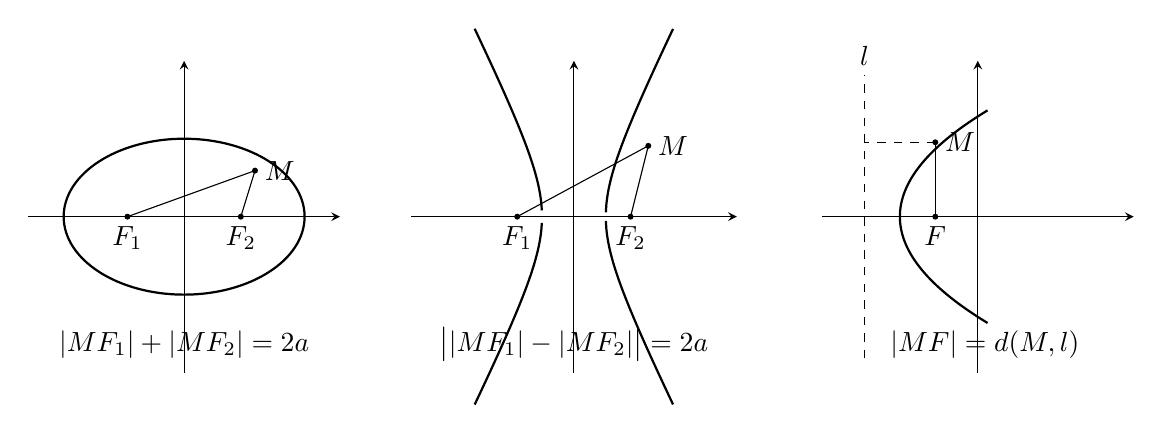
\begin{tikzpicture}[scale=0.9,>=stealth]
  % Ellipse
  \draw[->] (-5.2,0) -- (-0.8,0);
  \draw[->] (-3, -2.2) -- (-3,2.2);
  \draw[thick] (-3,0) ellipse (1.7 and 1.1);
  \fill (-3.8,0) circle (1.2pt) node[below] {$F_1$};
  \fill (-2.2,0) circle (1.2pt) node[below] {$F_2$};
  \fill (-2.0,0.65) circle (1.2pt) node[right] {$M$};
  \draw (-2.0,0.65) -- (-3.8,0);
  \draw (-2.0,0.65) -- (-2.2,0);
  \node at (-3,-1.8) {$|MF_1|+|MF_2|=2a$};

  % Hyperbola
  \draw[->] (0.2,0) -- (4.8,0);
  \draw[->] (2.5,-2.2) -- (2.5,2.2);
  \draw[thick,domain=-1.4:-0.451,samples=120,smooth] plot ({2.5+\x},{0.9*sqrt(\x*\x/0.45/0.45-1)});
  \draw[thick,domain=-1.4:-0.451,samples=120,smooth] plot ({2.5+\x},{-0.9*sqrt(\x*\x/0.45/0.45-1)});
  \draw[thick,domain=0.451:1.4,samples=120,smooth] plot ({2.5+\x},{0.9*sqrt(\x*\x/0.45/0.45-1)});
  \draw[thick,domain=0.451:1.4,samples=120,smooth] plot ({2.5+\x},{-0.9*sqrt(\x*\x/0.45/0.45-1)});
  \fill (1.7,0) circle (1.2pt) node[below] {$F_1$};
  \fill (3.3,0) circle (1.2pt) node[below] {$F_2$};
  \fill (3.55,1.0) circle (1.2pt) node[right] {$M$};
  \draw (3.55,1.0) -- (1.7,0);
  \draw (3.55,1.0) -- (3.3,0);
  \node at (2.5,-1.8) {$\bigl||MF_1|-|MF_2|\bigr|=2a$};

  % Parabola
  \draw[->] (6.0,0) -- (10.4,0);
  \draw[->] (8.2,-2.2) -- (8.2,2.2);
  \draw[thick,domain=-1.5:1.5,samples=120,smooth] plot ({7.1+0.55*\x*\x},{\x});
  \draw[dashed] (6.6,-2) -- (6.6,2) node[above] {$l$};
  \fill (7.6,0) circle (1.2pt) node[below] {$F$};
  \fill (7.6,1.05) circle (1.2pt) node[right] {$M$};
  \draw (7.6,1.05) -- (7.6,0);
  \draw[dashed] (7.6,1.05) -- (6.6,1.05);
  \node at (8.3,-1.8) {$|MF|=d(M,l)$};
\end{tikzpicture}

\end{center}

\subsection*{对应高考真题}

\begin{gaokao}{2016 年高考数学 全国I卷-理科第20题}

设圆$x^2+y^2+2x-15=0$的圆心为$A$，直线$l$过点$B(1,0)$且与$x$轴不重合，$l$交圆$A$于$C$，$D$两点，过$B$作$AC$的平行线交$AD$于点$E$．
（I）证明$|EA|+|EB|$为定值，并写出点$E$的轨迹方程；
（II）设点$E$的轨迹为曲线$C_1$，直线$l$交$C_1$于$M$，$N$两点，过$B$且与$l$垂直的直线与圆$A$交于$P$，$Q$两点，求四边形$MPNQ$面积的取值范围．

\begin{center}

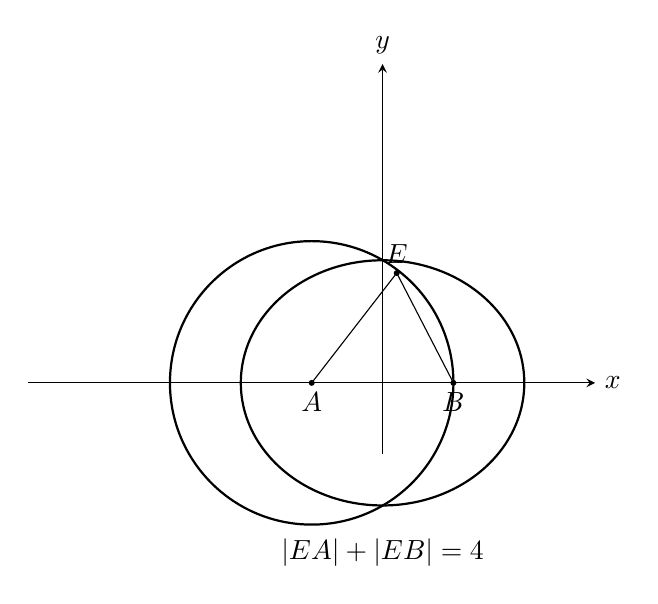
\begin{tikzpicture}[scale=0.9,>=stealth]
  \draw[->] (-5,0) -- (3,0) node[right] {$x$};
  \draw[->] (0,-1) -- (0,4.5) node[above] {$y$};
  \draw[thick] (-1,0) circle (2);
  \fill (-1,0) circle (1.2pt) node[below] {$A$};
  \fill (1,0) circle (1.2pt) node[below] {$B$};
  \draw[thick] (0,0) ellipse (2 and 1.73);
  \fill (0.2,1.55) circle (1.2pt) node[above] {$E$};
  \draw (0.2,1.55)--(-1,0);
  \draw (0.2,1.55)--(1,0);
  \node at (0,-2.4) {$|EA|+|EB|=4$};
\end{tikzpicture}

\end{center}

\paragraph{技巧对应}

第（I）问先证明 $|EA|+|EB|$ 为定值，再写出点 $E$ 的轨迹方程，这正是椭圆第一定义的直接应用：由两定点 $A,B$ 到动点 $E$ 的距离之和为常数，立即判断轨迹为以 $A,B$ 为焦点的椭圆。该题与本技巧的对应最直接、最完整，不仅有“识别定义”，还有“由定义写标准方程”的完整链条。

\paragraph{答案}

（I）$|EA|+|EB|=4$，轨迹方程为$\frac{x^2}{4}+\frac{y^2}{3}=1$（$y\neq0$）；（II）$[12,8\sqrt{3})$

\paragraph{解答}

解：（I）证明：圆$x^2+y^2+2x-15=0$即为$(x+1)^2+y^2=16$，可得圆心$A(-1,0)$，半径$r=4$，由$BE\parallel AC$，可得$\angle C=\angle EBD$，由$AC=AD$，可得$\angle D=\angle C$，即为$\angle D=\angle EBD$，即有$EB=ED$，则$|EA|+|EB|=|EA|+|ED|=|AD|=4$，故$E$的轨迹为以$A$，$B$为焦点的椭圆，且有$2a=4$，即$a=2$，$c=1$，$b=\sqrt{a^2-c^2}=\sqrt{3}$，则点$E$的轨迹方程为$\frac{x^2}{4}+\frac{y^2}{3}=1$（$y\neq0$）；（II）椭圆$C_1:\frac{x^2}{4}+\frac{y^2}{3}=1$，设直线$l:x=my+1$，由$PQ\perp l$，设$PQ:y=-m(x-1)$，由$\begin{cases}\frac{x^2}{4}+\frac{y^2}{3}=1\\x=my+1\end{cases}$可得$(3m^2+4)y^2+6my-9=0$，设$M(x_1,y_1)$，$N(x_2,y_2)$，可得$y_1+y_2=-\frac{6m}{3m^2+4}$，$y_1y_2=-\frac{9}{3m^2+4}$，则$|MN|=\sqrt{1+m^2}\cdot|y_1-y_2|=\sqrt{1+m^2}\cdot\sqrt{(y_1+y_2)^2-4y_1y_2}=\sqrt{1+m^2}\cdot\sqrt{\frac{36m^2}{(3m^2+4)^2}+\frac{36}{3m^2+4}}=12\cdot\frac{1+m^2}{3m^2+4}$，$A$到$PQ$的距离为$d=\frac{|0+m(-1-1)|}{\sqrt{1+m^2}}=\frac{|2m|}{\sqrt{1+m^2}}$，$|PQ|=2\sqrt{r^2-d^2}=2\sqrt{16-\frac{4m^2}{1+m^2}}=4\sqrt{\frac{3m^2+4}{1+m^2}}$，则四边形$MPNQ$面积为$S=\frac{1}{2}|PQ|\cdot|MN|=\frac{1}{2}\cdot4\sqrt{\frac{3m^2+4}{1+m^2}}\cdot12\cdot\frac{1+m^2}{3m^2+4}=24\sqrt{\frac{1+m^2}{3m^2+4}}=24\sqrt{\frac{1}{3+\frac{1}{1+m^2}}}$，当$m=0$时，$S$取得最小值$12$，又$\frac{1}{1+m^2}>0$，可得$S<24\sqrt{\frac{1}{3}}=8\sqrt{3}$，即有四边形$MPNQ$面积的取值范围是$[12,8\sqrt{3})$．

\par\smallskip\textcolor{gray}{\footnotesize 来源记录：\texttt{\detokenize{tex版(exam-zh模板2016-2025)/2016/2016-全国I卷-理科/questions.json}}}

\end{gaokao}

\begin{gaokao}{2021 年高考数学 上海春季卷第19题}

（1）团队在 $O$ 点西侧、东侧20千米处设有 $A$、$B$ 两站点，测量距离发现一点 $P$ 满足 $|PA|-|PB|=20$ 千米，可知 $P$ 在 $A$、$B$ 为焦点的双曲线上，以 $O$ 点为原点，东侧为 $x$ 轴正半轴，北侧为 $y$ 轴正半轴，建立平面直角坐标系，$P$ 在北偏东 $60^\circ$ 处，求双曲线标准方程和 $P$ 点坐标．\newline（2）团队又在南侧、北侧15千米处设有 $C$、$D$ 两站点，测量距离发现 $|QA|-|QB|=30$ 千米，$|QC|-|QD|=10$ 千米，求 $|OQ|$（精确到1米）和 $Q$ 点位置（精确到1米，$1^\circ$）

\begin{center}

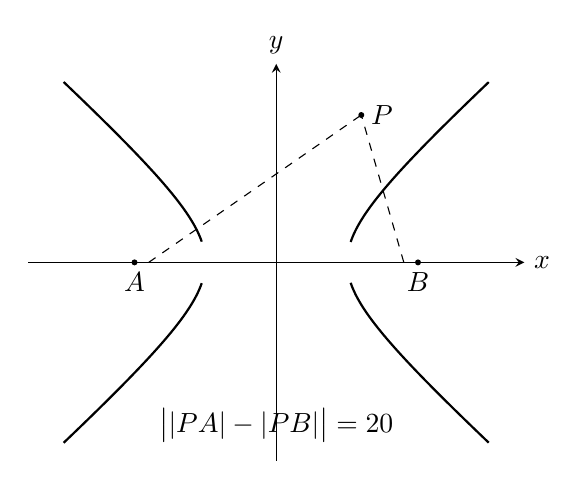
\begin{tikzpicture}[scale=0.9,>=stealth]
  \draw[->] (-3.5,0) -- (3.5,0) node[right] {$x$};
  \draw[->] (0,-2.8) -- (0,2.8) node[above] {$y$};
  \draw[thick,domain=-3:-1.05,samples=120,smooth] plot (\x,{0.9*sqrt(\x*\x-1)});
  \draw[thick,domain=-3:-1.05,samples=120,smooth] plot (\x,{-0.9*sqrt(\x*\x-1)});
  \draw[thick,domain=1.05:3,samples=120,smooth] plot (\x,{0.9*sqrt(\x*\x-1)});
  \draw[thick,domain=1.05:3,samples=120,smooth] plot (\x,{-0.9*sqrt(\x*\x-1)});
  \fill (-2,0) circle (1.2pt) node[below] {$A$};
  \fill (2,0) circle (1.2pt) node[below] {$B$};
  \draw[dashed] (1.8,0)--(1.2,2.08);
  \draw[dashed] (-1.8,0)--(1.2,2.08);
  \fill (1.2,2.08) circle (1.2pt) node[right] {$P$};
  \node at (0,-2.3) {$\bigl||PA|-|PB|\bigr|=20$};
\end{tikzpicture}

\end{center}

\paragraph{技巧对应}

题干中先后出现 $|PA|-|PB|=20$ 与 $|QA|-|QB|=30$、$|QC|-|QD|=10$，都是“到两个定点的距离差为定值”，这正对应双曲线第一定义。该题的价值在于：不需要先代数化简，只需先识别出轨迹类型，再由焦点位置与常数确定双曲线方程，能突出“看到距离差定值就想双曲线”的方法意识。

\paragraph{答案}

$(1)\ \frac{x^2}{100}-\frac{y^2}{300}=1,\ P(\frac{15\sqrt{2}}{2},\frac{5\sqrt{6}}{2})$；$(2)\ |OQ|\approx 19$ 米，$Q$ 点位置北偏东 $66^\circ$

\paragraph{解答}

（1）由题意可得 $a=10$，$c=20$，所以 $b^2=300$，所以双曲线的标准方程为 $\frac{x^2}{100}-\frac{y^2}{300}=1$，直线 $OP:y=\frac{\sqrt{3}}{3}x$，联立双曲线方程，可得 $x=\frac{15\sqrt{2}}{2}$，$y=\frac{5\sqrt{6}}{2}$，即点 $P$ 的坐标为 $(\frac{15\sqrt{2}}{2},\frac{5\sqrt{6}}{2})$．\newline（2）(1) $|QA|-|QB|=30$，则 $a=15$，$c=20$，所以 $b^2=175$，双曲线方程为 $\frac{x^2}{225}-\frac{y^2}{175}=1$；(2) $|QC|-|QD|=10$，则 $a=5$，$c=15$，所以 $b^2=200$，双曲线方程为 $\frac{y^2}{25}-\frac{x^2}{200}=1$，两双曲线方程联立，得 $Q(\frac{14400}{47},\frac{2975}{47})$，所以 $|OQ|\approx 19$ 米，$Q$ 点位置北偏东 $66^\circ$．

\par\smallskip\textcolor{gray}{\footnotesize 来源记录：\texttt{\detokenize{tex版(exam-zh模板2016-2025)/2021/2021-上海春季卷/questions.json}}}

\end{gaokao}

\begin{gaokao}{2019 年高考数学 全国II卷-文科第20题}

已知 $F_1,F_2$ 是椭圆 $C:\dfrac{x^2}{a^2}+\dfrac{y^2}{b^2}=1(a>b>0)$ 的两个焦点，$P$ 为 $C$ 上一点，$O$ 为坐标原点．
（1）若 $\triangle POF_2$ 为等边三角形，求 $C$ 的离心率；
（2）如果存在点 $P$，使得 $PF_1\perp PF_2$，且 $\triangle F_1PF_2$ 的面积等于 $16$，求 $b$ 的值和 $a$ 的取值范围．

\begin{center}

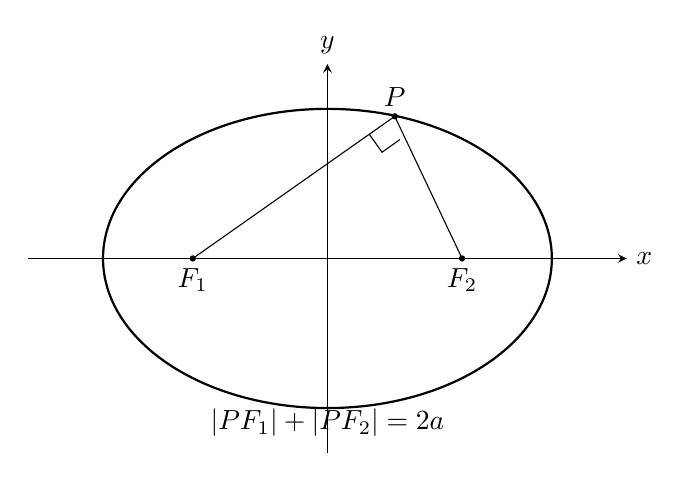
\begin{tikzpicture}[scale=0.95,>=stealth]
  \draw[->] (-4,0) -- (4,0) node[right] {$x$};
  \draw[->] (0,-2.6) -- (0,2.6) node[above] {$y$};
  \draw[thick] (0,0) ellipse (3 and 2);
  \fill (-1.8,0) circle (1.2pt) node[below] {$F_1$};
  \fill (1.8,0) circle (1.2pt) node[below] {$F_2$};
  \fill (0.9,1.9) circle (1.2pt) node[above] {$P$};
  \draw (-1.8,0)--(0.9,1.9);
  \draw (1.8,0)--(0.9,1.9);
  \draw (0.56,1.66)--(0.73,1.42)--(0.97,1.59);
  \node at (0,-2.2) {$|PF_1|+|PF_2|=2a$};
\end{tikzpicture}

\end{center}

\paragraph{技巧对应}

本题两问都紧扣椭圆焦点定义。第（1）问直接用椭圆上点满足 $|PF_1|+|PF_2|=2a$；第（2）问在 $PF_1\perp PF_2$ 的条件下，仍需结合椭圆第一定义处理焦点三角形中的长度关系。它不是单纯“判轨迹”，而是把第一定义作为椭圆性质来用，能体现本技巧在综合题中的深层作用。

\paragraph{答案}

（1）$e=\sqrt{3}-1$；（2）$b=4$，$a$ 的取值范围为 $[4\sqrt{2},+\infty)$

\paragraph{解答}

（1）连结 $PF_1$，由 $\triangle POF_2$ 为等边三角形可知：在 $\triangle F_1PF_2$ 中，$\angle F_1PF_2=90^\circ$，$PF_2=c$，$PF_1=\sqrt{3}c$，于是 $2a=PF_1+PF_2=c+\sqrt{3}c$，故椭圆 $C$ 的离心率为 $e=\dfrac{c}{a}=\dfrac{1}{1+\sqrt{3}}=\sqrt{3}-1$．
（2）由题意可知，满足条件的点 $P(x,y)$ 存在，当且仅当 $\dfrac{1}{2}|y|\cdot2c=16$，$\dfrac{y}{x+c}\cdot\dfrac{y}{x-c}=-1$，$\dfrac{x^2}{a^2}+\dfrac{y^2}{b^2}=1$，即 $c|y|=16$ (1)，$x^2+y^2=c^2$ (2)，$\dfrac{x^2}{a^2}+\dfrac{y^2}{b^2}=1$ (3)，由(2)(3)以及 $a^2=b^2+c^2$ 得 $y^2=\dfrac{b^4}{c^2}$，又由(1)知 $y^2=\dfrac{16^2}{c^2}$，故 $b=4$；由(2)(3)得 $x^2=\dfrac{a^2}{c^2}(c^2-b^2)$，所以 $c^2\ge b^2$，从而 $a^2=b^2+c^2\ge 2b^2=32$，故 $a\ge 4\sqrt{2}$；当 $b=4$，$a\ge 4\sqrt{2}$ 时，存在满足条件的点 $P$．所以 $b=4$，$a$ 的取值范围为 $[4\sqrt{2},+\infty)$．

\par\smallskip\textcolor{gray}{\footnotesize 来源记录：\texttt{\detokenize{tex版(exam-zh模板2016-2025)/2019/2019-全国II卷-文科/questions.json}}}

\end{gaokao}

\clearpage

\section{技巧45：圆锥曲线第二定义}

\subsection*{核心认识}

在平面内，若动点 $P$ 到定点 $F$ 的距离与它到定直线 $l$ 的距离之比为常数 $e$，且定点不在定直线上，则点 $P$ 的轨迹是圆锥曲线，其中 $F$ 为焦点，$l$ 为准线，$e$ 为离心率. 具体地：当 $0<e<1$ 时，轨迹是椭圆；当 $e>1$ 时，轨迹是双曲线；当 $e=1$ 时，轨迹是抛物线. 因而，题目中一旦出现“到定点的距离”和“到定直线的距离”的比为常数，就应优先联想到圆锥曲线第二定义；若已知点在某条抛物线上，也可反过来把“到焦点的距离”转化为“到准线的距离”.

\subsection*{操作步骤}

\begin{enumerate}

\item 先识别题干中是否同时出现“定点”“定直线”“距离之比为常数”这三个要素.

\item 若比值为常数 $e$，直接按 $e$ 的范围判断轨迹类型：$0<e<1$ 为椭圆，$e>1$ 为双曲线，$e=1$ 为抛物线.

\item 若题目已经给出具体圆锥曲线，先写出其焦点与准线，再把“点到焦点的距离”与“点到准线的距离”互相转化.

\item 求距离时注意：点到直线的距离常可由图形直接读出；若准线平行于坐标轴，常可直接用横坐标差或纵坐标差表示.

\item 最后不仅要得到数量关系，还要说明轨迹类型或所求结论对应的圆锥曲线性质.

\end{enumerate}

\subsection*{结构图}

\begin{center}

\begin{tikzpicture}[scale=0.95,>=stealth]
  % 椭圆
  \begin{scope}[xshift=0cm]
    \draw[->] (-2.8,0) -- (2.8,0);
    \draw[->] (0,-2.2) -- (0,2.2);
    \draw[thick] (0,0) ellipse (2 and 1.3);
    \draw[dashed] (1.6,-2) -- (1.6,2);
    \fill (1,0) circle (1.2pt) node[below] {$F$};
    \fill (0.8,1.2) circle (1.2pt) node[above] {$P$};
    \draw[dashed] (0.8,1.2) -- (1.6,1.2);
    \node[right] at (1.6,1.7) {$l$};
    \draw (1,0) -- (0.8,1.2);
    \node at (0,-1.8) {$0<e<1$};
    \node at (0,-2.05) {椭圆};
  \end{scope}
  % 双曲线
  \begin{scope}[xshift=6.2cm]
    \draw[->] (-2.8,0) -- (2.8,0);
    \draw[->] (0,-2.2) -- (0,2.2);
    \draw[domain=-2.5:-1.10,smooth,variable=\x,thick] plot ({\x},{0.9*sqrt((\x*\x/1.2)-1)});
    \draw[domain=-2.5:-1.10,smooth,variable=\x,thick] plot ({\x},{-0.9*sqrt((\x*\x/1.2)-1)});
    \draw[domain=1.10:2.5,smooth,variable=\x,thick] plot ({\x},{0.9*sqrt((\x*\x/1.2)-1)});
    \draw[domain=1.10:2.5,smooth,variable=\x,thick] plot ({\x},{-0.9*sqrt((\x*\x/1.2)-1)});
    \draw[dashed] (-0.9,-2) -- (-0.9,2);
    \fill (0.9,0) circle (1.2pt) node[below] {$F$};
    \fill (1.8,1.25) circle (1.2pt) node[above] {$P$};
    \draw[dashed] (1.8,1.25) -- (-0.9,1.25);
    \node[left] at (-0.9,1.7) {$l$};
    \draw (0.9,0) -- (1.8,1.25);
    \node at (0,-1.8) {$e>1$};
    \node at (0,-2.05) {双曲线};
  \end{scope}
  % 抛物线
  \begin{scope}[xshift=12.4cm]
    \draw[->] (-2.8,0) -- (2.8,0);
    \draw[->] (0,-2.2) -- (0,2.2);
    \draw[domain=-2:2,smooth,variable=\y,thick] plot ({0.25*\y*\y}, {\y});
    \draw[dashed] (-1,-2) -- (-1,2);
    \fill (1,0) circle (1.2pt) node[below] {$F$};
    \fill (1,2) circle (1.2pt) node[above] {$P$};
    \draw[dashed] (1,2) -- (-1,2);
    \node[left] at (-1,1.7) {$l$};
    \draw (1,0) -- (1,2);
    \node at (0,-1.8) {$e=1$};
    \node at (0,-2.05) {抛物线};
  \end{scope}
\end{tikzpicture}

\end{center}

\subsection*{对应高考真题}

\begin{gaokao}{2023 年高考数学 北京卷第6题}

已知抛物线 $C: y^2 = 8x$ 的焦点为 $F$ ，点 $M$ 在 $C$ 上．若 $M$ 到直线 $x = -3$ 的距离为 $5$，则 $|MF| =$ （ ）

\begin{enumerate}[label=\Alph*. ,itemsep=2pt]

\item $7$

\item $6$

\item $5$

\item $4$

\end{enumerate}

\begin{center}

\begin{tikzpicture}[scale=0.9,>=stealth]
  \draw[->] (-4,0) -- (5,0) node[right] {$x$};
  \draw[->] (0,-4) -- (0,4) node[above] {$y$};
  \draw[domain=-3.2:3.2,smooth,variable=\y,thick] plot ({\y*\y/8}, {\y});
  \draw[dashed] (-2,-3.8) -- (-2,3.8) node[above] {$x=-2$};
  \draw[dashed] (-3,-3.8) -- (-3,3.8) node[above] {$x=-3$};
  \fill (2,0) circle (1.2pt) node[below] {$F(2,0)$};
  \fill (1,2.828) circle (1.2pt) node[right] {$M$};
  \draw[dashed] (1,2.828) -- (-3,2.828);
  \draw (2,0) -- (1,2.828);
\end{tikzpicture}

\end{center}

\paragraph{技巧对应}

这道题与本技巧对应最直接. 题中已知点 $M$ 在抛物线 $C:y^2=8x$ 上，因此可立即调用抛物线第二定义：点到焦点的距离等于点到准线的距离. 先由方程得焦点 $F(2,0)$、准线 $x=-2$，再把“$M$ 到直线 $x=-3$ 的距离为 $5$”转化为“$M$ 到准线 $x=-2$ 的距离为 $4$”，从而直接得到 $|MF|=4$. 该题突出体现了第二定义的逆用：不必求点的坐标，也能迅速得到焦半径.

\paragraph{答案}

D

\paragraph{解答}

因为抛物线 $C: y^2 = 8x$ 的焦点 $F(2,0)$ ，准线方程为 $x = -2$ ，点 $M$ 在 $C$ 上，所以 $M$ 到准线 $x = -2$ 的距离为 $|MF|$，又 $M$ 到直线 $x = -3$ 的距离为 $5$，所以 $|MF| + 1 = 5$，故 $|MF| = 4$.

\par\smallskip\textcolor{gray}{\footnotesize 来源记录：\texttt{\detokenize{tex版(exam-zh模板2016-2025)/2023/2023-北京卷/questions.json}}}

\end{gaokao}

\begin{gaokao}{2022 年高考数学 全国乙卷-理科第5题}

设$F$为抛物线$C: y^2 = 4x$的焦点，点$A$在$C$上，点$B(3, 0)$，若$|AF| = |BF|$，则$|AB| =$（\qquad）

\begin{enumerate}[label=\Alph*. ,itemsep=2pt]

\item $2$

\item $2\sqrt{2}$

\item $3$

\item $3\sqrt{2}$

\end{enumerate}

\begin{center}

\begin{tikzpicture}[scale=1,>=stealth]
  \draw[->] (-2,0) -- (4.5,0) node[right] {$x$};
  \draw[->] (0,-3.5) -- (0,3.5) node[above] {$y$};
  \draw[domain=-3:3,smooth,variable=\y,thick] plot ({\y*\y/4}, {\y});
  \draw[dashed] (-1,-3.2) -- (-1,3.2) node[above] {$x=-1$};
  \fill (1,0) circle (1.2pt) node[below] {$F(1,0)$};
  \fill (3,0) circle (1.2pt) node[below] {$B(3,0)$};
  \fill (1,2) circle (1.2pt) node[right] {$A$};
  \draw[dashed] (1,2) -- (-1,2);
  \draw (1,0) -- (1,2);
  \draw (1,2) -- (3,0);
\end{tikzpicture}

\end{center}

\paragraph{技巧对应}

这道题的核心同样是抛物线第二定义. 由 $C:y^2=4x$ 可知焦点为 $F(1,0)$，准线为 $x=-1$. 题设 $|AF|=|BF|$，而 $B(3,0)$ 到焦点的距离易得为 $2$，于是 $|AF|=2$. 再由第二定义，点 $A$ 到准线的距离也为 $2$，故可直接确定 $A$ 的横坐标为 $1$，进而求出 $A$ 坐标与 $|AB|$. 这道题体现了“已知点在抛物线上，把焦点距离改写成准线距离”的标准用法.

\paragraph{答案}

B

\paragraph{解答}

由题意得，$F(1,0)$，则$|AF| = |BF| = 2$，\\即点$A$到准线$x=-1$的距离为2，所以点$A$的横坐标为$-1+2=1$，\\不妨设点$A$在$x$轴上方，代入得，$A(1,2)$，\\所以$|AB| = \sqrt{(3-1)^2 + (0-2)^2} = 2\sqrt{2}$.

\par\smallskip\textcolor{gray}{\footnotesize 来源记录：\texttt{\detokenize{tex版(exam-zh模板2016-2025)/2022/2022-全国乙卷-理科/questions.json}}}

\end{gaokao}

\begin{gaokao}{2025 年高考数学 全国II卷第6题}

设抛物线 $C:y^2=2px(p>0)$ 的焦点为 $F$，点 $A$ 在 $C$ 上，过 $A$ 作 $C$ 的准线的垂线，垂足为 $B$，若直线 $BF$ 的方程为 $y=-2x+2$，则 $|AF|=$（ ）

\begin{enumerate}[label=\Alph*. ,itemsep=2pt]

\item $3$

\item $4$

\item $5$

\item $6$

\end{enumerate}

\begin{center}

\begin{tikzpicture}[scale=0.95,>=stealth]
  \draw[->] (-2.5,0) -- (5,0) node[right] {$x$};
  \draw[->] (0,-1) -- (0,5.5) node[above] {$y$};
  \draw[domain=0:4.6,smooth,variable=\x,thick] plot ({\x},{sqrt(4*\x)});
  \draw[domain=0:4.6,smooth,variable=\x,thick] plot ({\x},{-sqrt(4*\x)});
  \draw[dashed] (-1,-0.8) -- (-1,5.2) node[above] {$x=-1$};
  \draw[thick] (-0.2,2.4) -- (2.2,-2.4) node[right] {$BF$};
  \fill (1,0) circle (1.2pt) node[below] {$F(1,0)$};
  \fill (-1,4) circle (1.2pt) node[left] {$B$};
  \fill (4,4) circle (1.2pt) node[right] {$A$};
  \draw[dashed] (4,4) -- (-1,4);
  \draw (1,0) -- (4,4);
\end{tikzpicture}

\end{center}

\paragraph{技巧对应}

这题比前两题多了一层几何转化，但本质仍是抛物线第二定义. 由直线 $BF$ 的方程先确定焦点 $F(1,0)$，从而得到抛物线 $C:y^2=4x$ 及准线 $x=-1$. 又因 $B$ 是点 $A$ 向准线所作垂线的垂足，所以 $AB$ 正是点 $A$ 到准线的距离. 根据第二定义，$|AF|=|AB|$. 题目再借助 $BF$ 的方程确定 $B$ 的位置，最终求出 $|AF|$. 该题很好地展示了第二定义与“准线垂足”信息的配合使用.

\paragraph{答案}

$C$

\paragraph{解答}

对 $l_{BF}:y=-2x+2$，令 $y=0$，则 $x=1$，所以 $F(1,0)$，$p=2$ 即抛物线 $C:y^2=4x$，故抛物线的准线方程为 $x=-1$，故 $B(-1,4)$，则 $y_A=4$，代入抛物线 $C:y^2=4x$ 得 $x_A=4$，所以 $AF=AB=x_A+\frac{p}{2}=4+1=5$.

\par\smallskip\textcolor{gray}{\footnotesize 来源记录：\texttt{\detokenize{tex版(exam-zh模板2016-2025)/2025/2025-全国II卷/questions.json}}}

\end{gaokao}

\clearpage

\section{技巧46：圆锥曲线第三定义}

\subsection*{核心认识}

在平面内，若动点 $P$ 与两个定点 $A,B$ 的连线斜率之积为常数，则常可用圆锥曲线第三定义判断轨迹或求离心率。设圆锥曲线中心在原点：

当焦点在 $x$ 轴上，且 $A,B$ 为左右顶点时，若 $P$ 在椭圆 $\dfrac{x^2}{a^2}+\dfrac{y^2}{b^2}=1$ 上，则
\[
k_{PA}k_{PB}=-\frac{b^2}{a^2}=e^2-1\quad(0<e<1).
\]
若 $P$ 在双曲线 $\dfrac{x^2}{a^2}-\dfrac{y^2}{b^2}=1$ 上，则
\[
k_{PA}k_{PB}=\frac{b^2}{a^2}=e^2-1\quad(e>1).
\]

当焦点在 $y$ 轴上，且 $A,B$ 为上、下顶点时，对应地有
\[
k_{PA}k_{PB}=-\frac{a^2}{b^2}=\frac{1}{e^2-1}\quad(\text{椭圆}),
\qquad
k_{PA}k_{PB}=\frac{a^2}{b^2}=\frac{1}{e^2-1}\quad(\text{双曲线}).
\]

因此，题目中若出现“过两个定点作连线，且斜率之积为定值”，就应优先联想到第三定义：负常数多对应椭圆，正常数多对应双曲线。原摘录中“看到平面内与两定点连线斜率之积等于常数的动点轨迹问题”这一判断是正确的。

\subsection*{操作步骤}

\begin{enumerate}

\item 先辨认两定点 $A,B$ 是否关于圆心对称，且常见为左右顶点或上、下顶点。

\item 再看已知量是“斜率之积为常数”还是“要求离心率/轨迹方程”。若是，就优先调用第三定义。

\item 若焦点在 $x$ 轴上：椭圆用 $k_{PA}k_{PB}=-\dfrac{b^2}{a^2}=e^2-1$，双曲线用 $k_{PA}k_{PB}=\dfrac{b^2}{a^2}=e^2-1$。

\item 若焦点在 $y$ 轴上：椭圆用 $k_{PA}k_{PB}=-\dfrac{a^2}{b^2}=\dfrac{1}{e^2-1}$，双曲线用 $k_{PA}k_{PB}=\dfrac{a^2}{b^2}=\dfrac{1}{e^2-1}$。

\item 若要求离心率，就把已知斜率积直接与上式对应，先求 $\dfrac{b^2}{a^2}$ 或 $\dfrac{a^2}{b^2}$，再求 $e$。

\item 若要求轨迹方程，可先由第三定义判断曲线类型，再写出标准方程；也可设 $P(x,y)$，把斜率积化简为标准方程，用来验证第三定义。

\end{enumerate}

\subsection*{结构图}

\begin{center}

\begin{tikzpicture}[scale=0.95]
  \draw[->] (-4.2,0) -- (4.2,0) node[right] {$x$};
  \draw[->] (0,-2.8) -- (0,2.8) node[above] {$y$};

  % ellipse
  \draw[thick,domain=0:360,samples=200,smooth] plot ({3*cos(\x)},{1.8*sin(\x)});

  % vertices and point
  \coordinate (A) at (-3,0);
  \coordinate (B) at (3,0);
  \coordinate (P) at (1.6,1.44);
  \coordinate (O) at (0,0);

  \fill (A) circle (1.4pt) node[below left] {$A(-a,0)$};
  \fill (B) circle (1.4pt) node[below right] {$B(a,0)$};
  \fill (P) circle (1.4pt) node[above right] {$P(x,y)$};
  \fill (O) circle (1.2pt) node[below left] {$O$};

  \draw[dashed] (P) -- (1.6,0) node[below] {};
  \draw[dashed] (P) -- (0,1.44);
  \draw[blue] (A) -- (P) node[midway,above left] {$k_{PA}$};
  \draw[blue] (B) -- (P) node[midway,above right] {$k_{PB}$};

  \node at (0,-2.2) {$\displaystyle k_{PA}k_{PB}=-\frac{b^2}{a^2}\ \text{(椭圆)}\qquad k_{PA}k_{PB}=\frac{b^2}{a^2}\ \text{(双曲线)}$};
\end{tikzpicture}

\end{center}

\subsection*{对应高考真题}

\begin{gaokao}{2022 年高考数学 全国甲卷-理科第10题}

椭圆 $C:\frac{x^2}{a^2}+\frac{y^2}{b^2}=1(a>b>0)$ 的左顶点为A，点P，Q均在C上，且关于y轴对称. 若直线AP, AQ的斜率之积为 $\frac{1}{4}$，则C的离心率为（ ）

\begin{enumerate}[label=\Alph*. ,itemsep=2pt]

\item $\frac{\sqrt{3}}{2}$

\item $\frac{\sqrt{2}}{2}$

\item $\frac{1}{2}$

\item $\frac{1}{3}$

\end{enumerate}

\begin{center}

\begin{tikzpicture}[scale=0.9]
  \draw[->] (-3.8,0) -- (3.8,0) node[right] {$x$};
  \draw[->] (0,-2.6) -- (0,2.6) node[above] {$y$};
  \draw[thick,domain=0:360,samples=200,smooth] plot ({3*cos(\x)},{2*sin(\x)});
  \coordinate (A) at (-3,0);
  \coordinate (P) at (1.5,1.5);
  \coordinate (Q) at (-1.5,1.5);
  \fill (A) circle (1.4pt) node[below left] {$A$};
  \fill (P) circle (1.4pt) node[above right] {$P$};
  \fill (Q) circle (1.4pt) node[above left] {$Q$};
  \draw[blue] (A) -- (P) node[midway,below] {$AP$};
  \draw[blue] (A) -- (Q) node[midway,left] {$AQ$};
  \draw[dashed] (P) -- (Q);
  \node at (0,-2.1) {$P,Q$ 关于 $y$ 轴对称，关注 $k_{AP}k_{AQ}$};
\end{tikzpicture}

\end{center}

\paragraph{技巧对应}

这题与该技巧是\textbf{完全对应}的。题设给出“椭圆 $C$ 的左顶点为 $A$，点 $P,Q$ 在 $C$ 上且关于 $y$ 轴对称，若直线 $AP,AQ$ 的斜率之积为 $\dfrac14$”，其中固定点 $A$ 与其对称关系共同构成了第三定义的典型场景。

从解法看，题目本质上正是在用
\[
k_{AP}k_{AQ}=-\frac{b^2}{a^2}
\]
这一关系求椭圆离心率。虽然原解答采用设点代算，但化简结果正好落到 $\dfrac{b^2}{a^2}=\dfrac14$，这正是第三定义的代数呈现，因此最适合作为本技巧的高考真题示范。

\paragraph{答案}

A

\paragraph{解答}

设$P(x_1,y_1)$，则$Q(-x_1,y_1)$，则由$k_{AP}\cdot k_{AQ}=\frac{1}{4}$得：$k_{AP}\cdot k_{AQ}=\frac{y_1}{x_1+a}\cdot\frac{y_1}{-x_1+a}=\frac{y_1^2}{-x_1^2+a^2}=\frac{1}{4}$. 由$\frac{x_1^2}{a^2}+\frac{y_1^2}{b^2}=1$得$y_1^2=\frac{b^2(a^2-x_1^2)}{a^2}$，代入得$\frac{b^2(a^2-x_1^2)}{a^2(-x_1^2+a^2)}=\frac{1}{4}$，即$\frac{b^2}{a^2}=\frac{1}{4}$，所以椭圆C的离心率$e=\frac{c}{a}=\sqrt{1-\frac{b^2}{a^2}}=\sqrt{1-\frac{1}{4}}=\frac{\sqrt{3}}{2}$. 故选A.

\par\smallskip\textcolor{gray}{\footnotesize 来源记录：\texttt{\detokenize{tex版(exam-zh模板2016-2025)/2022/2022-全国甲卷-理科/questions.json}}}

\end{gaokao}

\begin{gaokao}{2019 年高考数学 全国II卷-理科第21题}

已知点 $A(-2,0)$，$B(2,0)$，动点 $M(x,y)$ 满足直线 $AM$ 与 $BM$ 的斜率之积为 $-\frac{1}{2}$．记 $M$ 的轨迹为曲线 $C$．
（1）求 $C$ 的方程，并说明 $C$ 是什么曲线；
（2）过坐标原点的直线交 $C$ 于 $P$，$Q$ 两点，点 $P$ 在第一象限，$PE\perp x$ 轴，垂足为 $E$，连结 $QE$ 并延长交 $C$ 于点 $G$．
     （i）证明：$\triangle PQG$ 是直角三角形；
     （ii）求 $\triangle PQG$ 面积的最大值．

\begin{center}

\begin{tikzpicture}[scale=0.95]
  \draw[->] (-3.8,0) -- (3.8,0) node[right] {$x$};
  \draw[->] (0,-2.8) -- (0,2.8) node[above] {$y$};
  \draw[thick,domain=0:360,samples=200,smooth] plot ({2.8*cos(\x)},{2.0*sin(\x)});
  \coordinate (A) at (-2,0);
  \coordinate (B) at (2,0);
  \coordinate (M) at (1.2,1.6);
  \fill (A) circle (1.4pt) node[below left] {$A(-2,0)$};
  \fill (B) circle (1.4pt) node[below right] {$B(2,0)$};
  \fill (M) circle (1.4pt) node[above right] {$M(x,y)$};
  \draw[blue] (A) -- (M) node[midway,above left] {$AM$};
  \draw[blue] (B) -- (M) node[midway,above right] {$BM$};
  \node at (0,-2.25) {$k_{AM}k_{BM}=-\dfrac12$，对应椭圆第三定义};
\end{tikzpicture}

\end{center}

\paragraph{技巧对应}

这题与该技巧也有\textbf{实质且直接}的对应。第（1）问已知 $A(-2,0),B(2,0)$，动点 $M(x,y)$ 满足直线 $AM$ 与 $BM$ 的斜率之积为 $-\dfrac12$，要求轨迹方程并判断曲线类型。

这正是原摘录中“看到平面内与两定点连线斜率之积等于常数的动点轨迹问题”的标准模型。由
\[
k_{AM}k_{BM}=-\frac12
\]
立刻可联想到焦点在 $x$ 轴上的椭圆第三定义，即
\[
-\frac{b^2}{a^2}=-\frac12.
\]
于是可快速判断轨迹为椭圆，再得到对应标准方程。该题比上一题更能体现第三定义在“\textbf{识别轨迹类型}”中的作用。

\paragraph{答案}

（1）$\frac{x^2}{4}+\frac{y^2}{2}=1\ (|x|\neq 2)$，$C$ 为中心在坐标原点，焦点在 $x$ 轴上的椭圆，不含左右顶点；（2）（i）证明见解析；（ii）$\frac{16}{9}$

\paragraph{解答}

（1）直线 $AM$ 的斜率为 $\frac{y}{x+2}\ (x\neq -2)$，直线 $BM$ 的斜率为 $\frac{y}{x-2}\ (x\neq 2)$，由题意可知 $\frac{y}{x+2}\cdot\frac{y}{x-2}=-\frac{1}{2}$，化简得 $\frac{x^2}{4}+\frac{y^2}{2}=1\ (x\neq\pm 2)$，所以 $C$ 为中心在坐标原点，焦点在 $x$ 轴上的椭圆，不含左右顶点．
（2）（i）设直线 $PQ$ 的斜率为 $k$，则其方程为 $y=kx\ (k>0)$．由 $\begin{cases} y=kx \\ \frac{x^2}{4}+\frac{y^2}{2}=1 \end{cases}$ 得 $x=\pm\frac{2}{\sqrt{1+2k^2}}$．记 $u=\frac{2}{\sqrt{1+2k^2}}$，则 $P(u,uk)$，$Q(-u,-uk)$，$E(u,0)$．于是直线 $QG$ 的斜率为 $\frac{k}{2}$，方程为 $y=\frac{k}{2}(x-u)$．由 $\begin{cases} y=\frac{k}{2}(x-u) \\ \frac{x^2}{4}+\frac{y^2}{2}=1 \end{cases}$ 得 $(2+k^2)x^2-2uk^2x+k^2u^2-8=0$．(1) 设 $G(x_G,y_G)$，则 $-u$ 和 $x_G$ 是方程(1)的解，故 $x_G=\frac{u(3k^2+2)}{2+k^2}$，$y_G=\frac{uk^3}{2+k^2}$．从而直线 $PG$ 的斜率为 $\frac{\frac{uk^3}{2+k^2}-uk}{\frac{u(3k^2+2)}{2+k^2}-u}=-\frac{1}{k}$．所以 $PQ\perp PG$，即 $\triangle PQG$ 是直角三角形．
（ii）由（i）得 $|PQ|=2u\sqrt{1+k^2}$，$|PG|=\frac{2uk\sqrt{1+k^2}}{2+k^2}$，所以 $\triangle PQG$ 的面积 $S=\frac{1}{2}|PQ||PG|=\frac{8k(1+k^2)}{(1+2k^2)(2+k^2)}=\frac{8(\frac{1}{k}+k)}{1+2(\frac{1}{k}+k)^2}$．设 $t=k+\frac{1}{k}$，则由 $k>0$ 得 $t\geq 2$，当且仅当 $k=1$ 时取等号．因为 $S=\frac{8t}{1+2t^2}$ 在 $[2,+\infty)$ 单调递减，所以当 $t=2$，即 $k=1$ 时，$S$ 取得最大值 $\frac{16}{9}$．因此，$\triangle PQG$ 面积的最大值为 $\frac{16}{9}$．

\par\smallskip\textcolor{gray}{\footnotesize 来源记录：\texttt{\detokenize{tex版(exam-zh模板2016-2025)/2019/2019-全国II卷-理科/questions.json}}}

\end{gaokao}

\clearpage

\section{技巧47：手电筒模型}

\subsection*{核心认识}

在圆锥曲线中，若有一个定点 $P$，动直线与圆锥曲线交于两点 $A,B$，再连接 $PA,PB$，并且题目给出 $PA,PB$ 的斜率和或斜率积为定值，就要优先想到“由两束射线反推弦 $AB$ 的不变量”：通常结论是弦 $AB$ 斜率为定值，或弦 $AB$ 恒过定点。这一结构像定点 $P$ 发出两束光照到曲线上，故称“手电筒模型”。

就本页摘录可直接整理出的高中层面常用结论看：

1. 对椭圆 $\dfrac{x^2}{a^2}+\dfrac{y^2}{b^2}=1$，若定点为 $P(x_0,y_0)$，直线 $PA,PB$ 的斜率分别为 $k_1,k_2$，当 $k_1+k_2=\lambda\,(\lambda\ne 0)$ 时，弦 $AB$ 过定点
\[
\left(x_0-\frac{2y_0}{\lambda},\,-y_0-\frac{2b^2x_0}{\lambda a^2}\right).
\]
2. 当 $k_1+k_2=0$ 时，常可转化为弦 $AB$ 的斜率为定值。
3. 当 $k_1k_2$ 为定值时，也常能推出弦 $AB$ 斜率恒定或恒过定点，但具体公式要按椭圆、双曲线、抛物线分别使用。

OCR中有两点需特别校正：其一，摘录中“若 $k_1\cdot k_2=1-e^2$ 时”的抛物线一行与左侧条件对应关系有版面歧义，不能直接照抄使用；其二，例题后半页混入了别的栏目标题，不属于题意本身。讲义使用时，应以“定点 $P$ + 两条连线斜率和/积为定值 $\Rightarrow$ 弦的定点或定斜率性质”为核心，不机械背诵残缺公式。

\subsection*{操作步骤}

\begin{enumerate}

\item 先辨型：看是否存在一个定点 $P$，以及一条动直线与圆锥曲线交于两点 $A,B$，再看题目是否给出 $k_{PA}+k_{PB}$ 或 $k_{PA}k_{PB}$ 为定值。

\item 若已知圆锥曲线标准方程和定点坐标，优先把题目与现成模型对照：是“斜率和为定值”，还是“斜率积为定值”；是椭圆、双曲线，还是抛物线。

\item 若题目正好对应结论型模型，则直接写出弦 $AB$ 的定点或定斜率结论，再代入参数化简。

\item 若题目没有完全落入现成公式，也可保留“手电筒模型”的思路：设动直线方程，与曲线联立，利用韦达定理表示两交点，再把 $k_{PA}+k_{PB}$ 或 $k_{PA}k_{PB}$ 化成关于直线参数的关系。

\item 整理得到的关系后，若能化为直线方程的点斜式或一般式中某点恒满足，就得到“过定点”；若能化为斜率与参数无关，就得到“定斜率”。

\item 得到结论后要补检验：斜率不存在、重合点、切线情形、题设排除的特殊位置，通常需要单独说明。

\end{enumerate}

\subsection*{结构图}

\begin{center}

\begin{tikzpicture}[scale=0.9,>=stealth]
  \draw[->] (-4.5,0)--(4.8,0) node[right]{$x$};
  \draw[->] (0,-3.2)--(0,3.6) node[above]{$y$};
  \draw[thick] (0,0) ellipse (3.6 and 2.2);
  \coordinate (P) at (0.8,1.2);
  \coordinate (A) at (-2.6,1.5);
  \coordinate (B) at (3.1,-1.1);
  \draw[thick] (A)--(B);
  \draw[thick] (P)--(A);
  \draw[thick] (P)--(B);
  \fill (P) circle (1.5pt) node[above right]{$P(x_0,y_0)$};
  \fill (A) circle (1.5pt) node[above left]{$A$};
  \fill (B) circle (1.5pt) node[below right]{$B$};
  \node at (-1.1,2.25) {$k_1$};
  \node at (2.25,0.45) {$k_2$};
  \node at (0.9,-1.45) {$AB$};
  \node at (2.7,2.8) {若 $k_1+k_2$ 或 $k_1k_2$ 为定值};
  \node at (2.45,2.35) {则常推出弦 $AB$ 的不变量};
\end{tikzpicture}

\end{center}

\subsection*{对应高考真题}

\begin{gaokao}{2017 年高考数学 全国I卷-理科第20题}

已知椭圆 $C:\frac{x^2}{a^2}+\frac{y^2}{b^2}=1$（$a>b>0$），四点 $P_1(1,1)$，$P_2(0,1)$，$P_3(-1,\frac{\sqrt{3}}{2})$，$P_4(1,\frac{\sqrt{3}}{2})$ 中恰有三点在椭圆 $C$ 上．
（1）求 $C$ 的方程；
（2）设直线 $l$ 不经过 $P_2$ 点且与 $C$ 相交于 $A$，$B$ 两点．若直线 $P_2A$ 与直线 $P_2B$ 的斜率的和为 $-1$，证明：$l$ 过定点．

\begin{center}

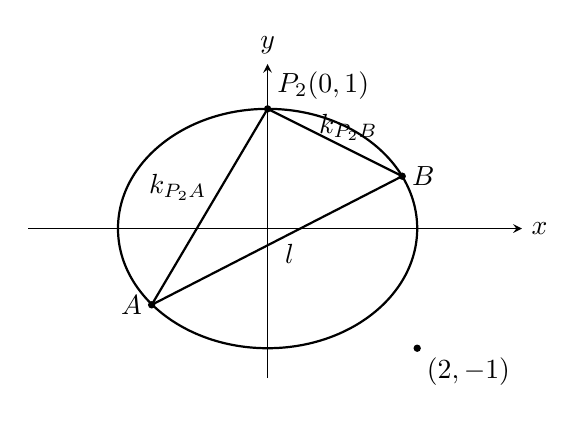
\begin{tikzpicture}[scale=0.95,>=stealth]
  \draw[->] (-3.2,0)--(3.4,0) node[right]{$x$};
  \draw[->] (0,-2.0)--(0,2.2) node[above]{$y$};
  \draw[thick] (0,0) ellipse (2 and 1.6);
  \coordinate (P2) at (0,1.6);
  \coordinate (A) at (-1.55,-1.02);
  \coordinate (B) at (1.8,0.7);
  \coordinate (D) at (2,-1.6);
  \draw[thick] (A)--(B) node[pos=0.55,below]{$l$};
  \draw[thick] (P2)--(A);
  \draw[thick] (P2)--(B);
  \fill (P2) circle (1.4pt) node[above right]{$P_2(0,1)$};
  \fill (A) circle (1.4pt) node[left]{$A$};
  \fill (B) circle (1.4pt) node[right]{$B$};
  \fill (D) circle (1.4pt) node[below right]{$(2,-1)$};
  \node at (-1.2,0.55) {$k_{P_2A}$};
  \node at (1.08,1.35) {$k_{P_2B}$};
\end{tikzpicture}

\end{center}

\paragraph{技巧对应}

这道题与“手电筒模型”是高度同构的典型题。题中定点是 $P_2(0,1)$，动直线 $l$ 与椭圆交于 $A,B$ 两点，且给出 $k_{P_2A}+k_{P_2B}=-1$ 为定值，正对应摘录中“椭圆里，从定点向两动点引线，若斜率和为定值，则弦 $AB$ 过定点”的结论。

把椭圆方程先求出为 $\dfrac{x^2}{4}+y^2=1$，于是 $a^2=4,b^2=1$，定点 $P_2(0,1)$ 即 $x_0=0,y_0=1$，又 $\lambda=-1$。代入摘录中的椭圆结论
\[
\left(x_0-\frac{2y_0}{\lambda},-y_0-\frac{2b^2x_0}{\lambda a^2}\right)
\]
可得定点
\[
\left(0-\frac{2\cdot 1}{-1},-1-\frac{2\cdot 1\cdot 0}{(-1)\cdot 4}\right)=(2,-1),
\]
与题目答案完全一致。因此这题几乎就是该模型的标准落地：题目原解用联立与韦达定理完成证明，而技巧法可直接缩短判断路径。

\paragraph{答案}

（1）$\frac{x^2}{4}+y^2=1$；（2）证明见解析，定点为 $(2,-1)$

\paragraph{解答}

解：（1）根据椭圆的对称性，$P_3(-1,\frac{\sqrt{3}}{2})$，$P_4(1,\frac{\sqrt{3}}{2})$ 两点必在椭圆 $C$ 上，又 $P_4$ 的横坐标为 1，\ensuremath{\therefore}椭圆必不过 $P_1(1,1)$，\ensuremath{\therefore}$P_2(0,1)$，$P_3(-1,\frac{\sqrt{3}}{2})$，$P_4(1,\frac{\sqrt{3}}{2})$ 三点在椭圆 $C$ 上．把 $P_2(0,1)$，$P_3(-1,\frac{\sqrt{3}}{2})$ 代入椭圆 $C$，得：$\begin{cases} \frac{0}{a^2}+\frac{1}{b^2}=1 \\ \frac{1}{a^2}+\frac{3}{4b^2}=1 \end{cases}$，解得 $a^2=4$，$b^2=1$，\ensuremath{\therefore}椭圆 $C$ 的方程为 $\frac{x^2}{4}+y^2=1$．
证明：（2）(1)当斜率不存在时，设 $l:x=m$，$A(m,y_A)$，$B(m,-y_A)$，\ensuremath{\because}直线 $P_2A$ 与直线 $P_2B$ 的斜率的和为 $-1$，\ensuremath{\therefore}$\frac{y_A-1}{m-0}+\frac{-y_A-1}{m-0}=\frac{-2}{m}=-1$，解得 $m=2$，此时 $l$ 过椭圆右顶点，不存在两个交点，故不满足．(2)当斜率存在时，设 $l:y=kx+t$，($t\neq1$)，$A(x_1,y_1)$，$B(x_2,y_2)$，联立 $\begin{cases} y=kx+t \\ \frac{x^2}{4}+y^2=1 \end{cases}$，整理，得 $(1+4k^2)x^2+8ktx+4t^2-4=0$，$\Delta>0$，$x_1+x_2=-\frac{8kt}{1+4k^2}$，$x_1x_2=\frac{4t^2-4}{1+4k^2}$，则 $k_{P_2A}+k_{P_2B}=\frac{y_1-1}{x_1}+\frac{y_2-1}{x_2}=\frac{kx_1+t-1}{x_1}+\frac{kx_2+t-1}{x_2}=2k+\frac{t-1}{x_1}+\frac{t-1}{x_2}=2k+(t-1)\frac{x_1+x_2}{x_1x_2}=2k+(t-1)\frac{-\frac{8kt}{1+4k^2}}{\frac{4t^2-4}{1+4k^2}}=2k-\frac{2k(t-1)}{t+1}=\frac{2k(t+1)-2k(t-1)}{t+1}=\frac{4k}{t+1}=-1$，又 $t\neq1$，\ensuremath{\therefore}$t=-2k-1$，此时 $\Delta=64k^2-16(1+4k^2)(t^2-1)$，代入得 $\Delta=-64k$，存在 $k$，使得 $\Delta>0$ 成立，\ensuremath{\therefore}直线 $l$ 的方程为 $y=kx-2k-1$，当 $x=2$ 时，$y=-1$，\ensuremath{\therefore}$l$ 过定点 $(2,-1)$．

\par\smallskip\textcolor{gray}{\footnotesize 来源记录：\texttt{\detokenize{tex版(exam-zh模板2016-2025)/2017/2017-全国I卷-理科/questions.json}}}

\end{gaokao}

\begin{gaokao}{2020 年高考数学 全国I卷-理科第20题}

已知$A,B$分别为椭圆$E:\frac{x^2}{a^2}+y^2=1(a>1)$的左、右顶点，$G$为$E$的上顶点，$\overrightarrow{AG}\cdot\overrightarrow{GB}=8$。$P$为直线$x=6$上的动点，$PA$与$E$的另一交点为$C$，$PB$与$E$的另一交点为$D$。
(1)求$E$的方程；
(2)证明：直线$CD$过定点。

\begin{center}

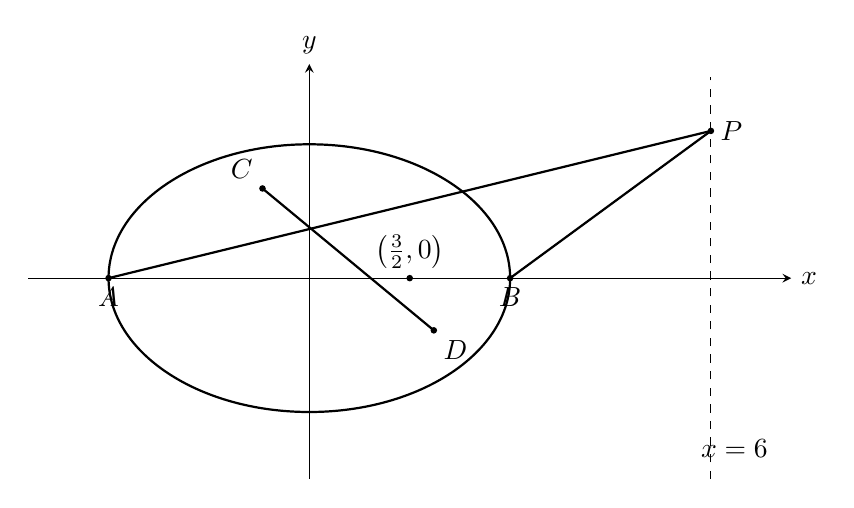
\begin{tikzpicture}[scale=0.85,>=stealth]
  \draw[->] (-4.2,0)--(7.2,0) node[right]{$x$};
  \draw[->] (0,-3.0)--(0,3.2) node[above]{$y$};
  \draw[thick] (0,0) ellipse (3 and 2);
  \coordinate (A) at (-3,0);
  \coordinate (B) at (3,0);
  \coordinate (P) at (6,2.2);
  \coordinate (C) at (-0.7,1.34);
  \coordinate (D) at (1.86,-0.78);
  \coordinate (F) at (1.5,0);
  \draw[thick] (P)--(A);
  \draw[thick] (P)--(B);
  \draw[thick] (C)--(D);
  \fill (A) circle (1.4pt) node[below]{$A$};
  \fill (B) circle (1.4pt) node[below]{$B$};
  \fill (P) circle (1.4pt) node[right]{$P$};
  \fill (C) circle (1.4pt) node[above left]{$C$};
  \fill (D) circle (1.4pt) node[below right]{$D$};
  \fill (F) circle (1.4pt) node[above]{$\left(\frac{3}{2},0\right)$};
  \draw[dashed] (6,-3)--(6,3);
  \node at (6.35,-2.55) {$x=6$};
\end{tikzpicture}

\end{center}

\paragraph{技巧对应}

这道题不是摘录中“斜率和/积为定值”的原型题，但与该模型有实质共通性，适合作为同类拓展。题中定点是动点 $P(6,y_0)$，分别连到椭圆两个固定顶点 $A,B$，再由直线 $PA,PB$ 与椭圆的另一个交点得到 $C,D$，最终证明弦 $CD$ 过定点。其核心仍然是“以一个点为光源，发出两束线，借两交点之间的弦寻找不变量”。

与技巧47的对应关系在于：虽然题设没有直接给出 $k_{PA}+k_{PB}$ 或 $k_{PA}k_{PB}$ 为定值，但整体结构仍是“定点（此处对每个位置的 $P$ 而言）$\to$ 两条射线 $\to$ 曲线上两点 $\to$ 弦的不变量”。它能帮助学生把“过定点”的结论视为同一类几何机制，而不只局限于公式套用。

不过从贴合度看，这题弱于 2017 年全国 I 卷理科第 20 题，因为它主要靠代数求点坐标再消元，不是斜率和/积触发的标准手电筒结论。故本题更适合作为“同结构迁移题”，不宜作为首选例题。

\paragraph{答案}

(1)$\frac{x^2}{9}+y^2=1$；(2)直线$CD$过定点$\left(\frac{3}{2},0\right)$

\paragraph{解答}

(1)由椭圆方程得$A(-a,0),B(a,0),G(0,1)$，则$\overrightarrow{AG}=(a,1),\overrightarrow{GB}=(a,-1)$，$\overrightarrow{AG}\cdot\overrightarrow{GB}=a^2-1=8$，解得$a^2=9$，故椭圆方程为$\frac{x^2}{9}+y^2=1$。
(2)设$P(6,y_0)$，则直线$AP$方程为$y=\frac{y_0}{9}(x+3)$，与椭圆联立得$(y_0^2+9)x^2+6y_0^2x+9y_0^2-81=0$，由韦达定理$x_A\cdot x_C=\frac{9y_0^2-81}{y_0^2+9}$，而$x_A=-3$，得$x_C=\frac{-3y_0^2+27}{y_0^2+9}$，代入得$y_C=\frac{6y_0}{y_0^2+9}$，故$C\left(\frac{-3y_0^2+27}{y_0^2+9},\frac{6y_0}{y_0^2+9}\right)$。同理直线$PB$方程$y=\frac{y_0}{3}(x-3)$，与椭圆联立得$D\left(\frac{3y_0^2-3}{y_0^2+1},\frac{-2y_0}{y_0^2+1}\right)$。当$y_0\neq0$时，直线$CD$斜率$k=\frac{\frac{6y_0}{y_0^2+9}-\frac{-2y_0}{y_0^2+1}}{\frac{-3y_0^2+27}{y_0^2+9}-\frac{3y_0^2-3}{y_0^2+1}}=\frac{4y_0}{3(3-y_0^2)}$，直线$CD$方程为$y-\frac{-2y_0}{y_0^2+1}=\frac{4y_0}{3(3-y_0^2)}\left(x-\frac{3y_0^2-3}{y_0^2+1}\right)$，化简得$y=\frac{4y_0}{3(3-y_0^2)}\left(x-\frac{3}{2}\right)$，故过定点$\left(\frac{3}{2},0\right)$。当$y_0=0$时，$C(3,0),D(3,0)$，直线$CD$为$x=3$，也过$\left(\frac{3}{2},0\right)$。综上，直线$CD$过定点$\left(\frac{3}{2},0\right)$。

\par\smallskip\textcolor{gray}{\footnotesize 来源记录：\texttt{\detokenize{tex版(exam-zh模板2016-2025)/2020/2020-全国I卷-理科/questions.json}}}

\end{gaokao}

\clearpage

\section{技巧48：阿基米德三角形}

\subsection*{核心认识}

阿基米德三角形，指圆锥曲线的一条弦与该弦两端点处切线所围成的三角形。对椭圆、双曲线，通常记弦为 $AB$，两切线交于 $Q$，得到 $\triangle ABQ$；对抛物线，通常记两切线交于 $P$，得到 $\triangle ABP$。

本技巧的识别标志是：题目同时出现“圆锥曲线上的两点”“过这两点作切线”“两切线交点”“弦经过定点或焦点”“求轨迹、定点、垂直、面积最值”等信息。此时应主动把“弦 $AB$ 与切线交点”整体看成阿基米德三角形，而不是把切线、弦、焦点分散处理。

原摘录中有明显的 OCR 混乱，需作如下规范：

1. 抛物线部分应统一为：已知抛物线 $y^2=2px\,(p>0)$ 的弦 $AB$，过 $A,B$ 分别作抛物线的切线，两切线交于点 $P$，则 $\triangle ABP$ 为抛物线中的阿基米德三角形。
2. 当抛物线的弦 $AB$ 经过焦点 $F$ 时，顶点 $P$ 在准线上，且这是最常用的特殊情形。
3. 椭圆、双曲线中，若弦 $AB$ 过焦点，则切线交点落在对应准线上，并且连接“焦点与切线交点”的线段垂直于弦 $AB$。

解题价值主要体现在两类转化：一类是把“切线条件”转化为“切点参数关系或交点轨迹”；另一类是把“弦过焦点”转化为“顶点在准线、且与弦垂直”这一强几何性质，从而快速求点、求长、求面积。

\subsection*{操作步骤}

\begin{enumerate}

\item 先判断是否出现“弦的两个端点处作切线，切线相交”这一结构；若出现，就优先联想到阿基米德三角形。

\item 若是椭圆或双曲线，重点检查弦 $AB$ 是否过某个定点 $P(m,0)$；若过焦点，则切线交点在对应准线上，这是求轨迹、定点的直接入口。

\item 若是抛物线，重点检查弦 $AB$ 是否过焦点 $F$；若经过焦点，则切线交点 $P$ 在准线上，且 $PF\perp AB$，常可据此设出点 $P$ 的坐标。

\item 遇到面积问题时，优先把三角形面积写成“底乘高”的形式；其中底边常取弦 $AB$，高常利用“交点在准线”或“垂直关系”来确定。

\item 遇到轨迹或定点问题时，不急于分别求两条切线；应先把弦的方程与圆锥曲线联立，再利用阿基米德三角形的整体性质确定交点所在直线。

\item 若题中已给出焦点、准线、过焦点的弦、切线交点等信息，可优先走几何性质；只有在性质不足以闭合时，再回到坐标联立计算。

\end{enumerate}

\subsection*{结构图}

\begin{center}

\begin{tikzpicture}[scale=0.9]
  \draw[->] (-2.2,0) -- (6.2,0) node[right] {$x$};
  \draw[->] (0,-3.2) -- (0,3.2) node[above] {$y$};
  \draw[dashed] (-1,-3) -- (-1,3) node[above] {$x=-1$};
  \draw[thick,domain=0:4.8,samples=200] plot (\x,{2*sqrt(\x)});
  \draw[thick,domain=0:4.8,samples=200] plot (\x,{-2*sqrt(\x)});
  \coordinate (F) at (1,0);
  \coordinate (A) at (4,4);
  \coordinate (B) at (0.25,-1);
  \coordinate (P) at (-1,1.5);
  \draw[thick] (P)--(A) (P)--(B) (A)--(B) (P)--(F);
  \fill (F) circle (1.2pt) node[below right] {$F$};
  \fill (A) circle (1.2pt) node[above right] {$A$};
  \fill (B) circle (1.2pt) node[below right] {$B$};
  \fill (P) circle (1.2pt) node[above left] {$P$};
  \node at (2.8,2.7) {$y^2=4x$};
  \draw ($(F)+(0.18,0.18)$) -- ($(F)+(-0.02,0.38)$) -- ($(F)+(-0.22,0.18)$);
  \node at (2.0,-1.9) {$AB$ 过焦点时，$P$ 在准线上，且 $PF\perp AB$};
\end{tikzpicture}

\end{center}

\subsection*{对应高考真题}

\begin{gaokao}{2021 年高考数学 全国乙卷-理科第21题}

已知抛物线$C:x^2=2py$（$p>0$）的焦点为$F$，且$F$与圆$M:x^2+(y+4)^2=1$上点的距离的最小值为4。
（1）求$p$；
（2）若点$P$在$M$上，$PA$，$PB$是$C$的两条切线，$A$，$B$是切点，求$\triangle PAB$面积的最大值。

\paragraph{技巧对应}

这道题与抛物线中的阿基米德三角形对应最直接。题目已明确给出：点 $P$ 在定圆上，$PA,PB$ 是抛物线的两条切线，$A,B$ 为切点，于是天然形成阿基米德三角形 $\triangle PAB$。第（2）问要求三角形面积最大值，正对应原摘录中“抛物线中的阿基米德三角形”关于面积问题的典型应用场景。

从方法上看，本题虽然标准解答主要使用坐标联立，但若教学中引入阿基米德三角形视角，学生能更快抓住结构核心：$P$ 是三角形顶点，$AB$ 是抛物线的一条弦，而两边 $PA,PB$ 恰是切线。这样处理时，面积公式、弦方程、切线关系不再是零散结论，而是统一服务于同一个几何对象，十分适合作为本技巧的真题支撑。

\paragraph{答案}

（1）$p=2$；（2）$20\sqrt{5}$

\paragraph{解答}

（1）焦点$F(0,\frac{p}{2})$到圆$x^2+(y+4)^2=1$的最短距离为$\frac{p}{2}+3=4$，所以$p=2$。
（2）抛物线$y=\frac14x^2$，设$A(x_1,y_1)$，$B(x_2,y_2)$，$P(x_0,y_0)$，得$l_{PA}: y=\frac12x_1(x-x_1)+y_1=\frac12x_1x-\frac14x_1^2=\frac12x_1x-y_1$，$l_{PB}: y=\frac12x_2x-y_2$，且$x_0^2=-y_0^2-8y_0-15$。$l_{PA}$，$l_{PB}$都过点$P(x_0,y_0)$，则$\begin{cases} y_0=\frac12x_1x_0-y_1 \\ y_0=\frac12x_2x_0-y_2 \end{cases}$，故$l_{AB}: y_0=\frac12x_0x-y$，即$y=\frac12x_0x-y_0$。联立$\begin{cases} y=\frac12x_0x-y_0 \\ x^2=4y \end{cases}$，得$x^2-2x_0x+4y_0=0$，$\Delta=4x_0^2-16y_0$。所以$|AB|=\sqrt{1+\frac{x_0^2}{4}}\cdot\sqrt{4x_0^2-16y_0}=\sqrt{4+x_0^2}\cdot\sqrt{x_0^2-4y_0}$，$d_{P\to AB}=\frac{|x_0^2-4y_0|}{\sqrt{x_0^2+4}}$，所以$S_{\triangle PAB}=\frac12|AB|\cdot d_{P\to AB}=\frac12\sqrt{x_0^2-4y_0}\cdot\sqrt{x_0^2-4y_0}=\frac12(x_0^2-4y_0)^{\frac32}=\frac12(-y_0^2-12y_0-15)^{\frac32}$。而$y_0\in[-5,-3]$，故当$y_0=-5$时，$S_{\triangle PAB}$达到最大，最大值为$20\sqrt{5}$。

\par\smallskip\textcolor{gray}{\footnotesize 来源记录：\texttt{\detokenize{tex版(exam-zh模板2016-2025)/2021/2021-全国乙卷-理科/questions.json}}}

\end{gaokao}

\begin{gaokao}{2019 年高考数学 全国III卷-理科第21题}

已知曲线 $C: y=\dfrac{x^2}{2}$，$D$ 为直线 $y=-\dfrac{1}{2}$ 上的动点，过 $D$ 作 $C$ 的两条切线，切点分别为 $A$，$B$。
（1）证明：直线 $AB$ 过定点；
（2）若以 $E\left(0,\dfrac{5}{2}\right)$ 为圆心的圆与直线 $AB$ 相切，且切点为线段 $AB$ 的中点，求四边形 $ADBE$ 的面积。

\begin{center}

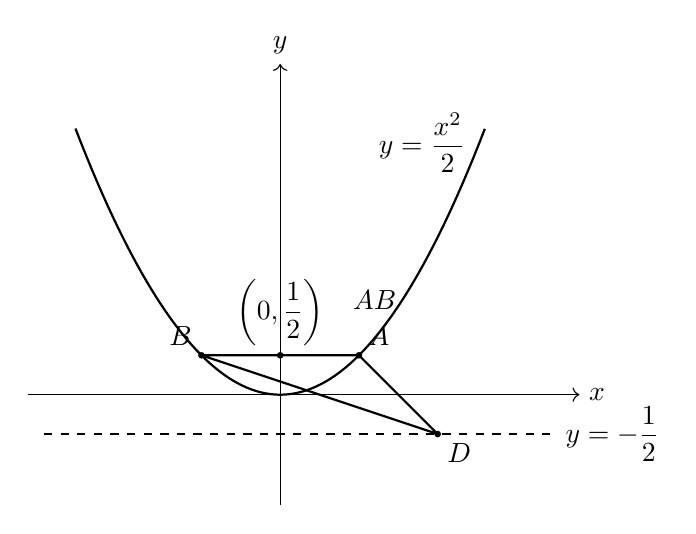
\begin{tikzpicture}[scale=1.0]
  \draw[->] (-3.2,0) -- (3.8,0) node[right] {$x$};
  \draw[->] (0,-1.4) -- (0,4.2) node[above] {$y$};
  \draw[thick,domain=-2.6:2.6,samples=200] plot (\x,{0.5*\x*\x});
  \draw[dashed] (-3,-0.5) -- (3.5,-0.5) node[right] {$y=-\dfrac12$};
  \coordinate (D) at (2,-0.5);
  \coordinate (A) at (1,0.5);
  \coordinate (B) at (-1,0.5);
  \coordinate (T) at (0,0.5);
  \draw[thick] (D)--(A) (D)--(B) (A)--(B);
  \fill (D) circle (1.2pt) node[below right] {$D$};
  \fill (A) circle (1.2pt) node[above right] {$A$};
  \fill (B) circle (1.2pt) node[above left] {$B$};
  \fill (T) circle (1.2pt) node[above] {$\left(0,\dfrac12\right)$};
  \node at (1.8,3.2) {$y=\dfrac{x^2}{2}$};
  \node at (1.2,1.2) {$AB$};
\end{tikzpicture}

\end{center}

\paragraph{技巧对应}

这道题与原摘录中“若直线 $l$ 与抛物线没有公共点，以 $l$ 上的点为顶点的阿基米德三角形的底边 $AB$ 经过定点”高度对应。题中点 $D$ 在直线 $y=-\dfrac12$ 上运动，过 $D$ 作抛物线 $C:y=\dfrac{x^2}{2}$ 的两条切线，切点为 $A,B$，于是 $\triangle DAB$ 正是抛物线中的阿基米德三角形。

第（1）问证明直线 $AB$ 过定点，正是该技巧中最有代表性的“顶点在线上动，底边过定点”模型；第（2）问继续讨论中点、切圆、面积，体现了阿基米德三角形在定点、对称与面积计算中的综合作用。相较于一般切线题，本题更能突出“先识别阿基米德三角形，再整体处理”的方法价值。

\paragraph{答案}

（1）定点为 $\left(0,\dfrac{1}{2}\right)$；（2）四边形 $ADBE$ 的面积为 $3$ 或 $4\sqrt{2}$。

\paragraph{解答}

（1）设 $D\left(t,-\dfrac{1}{2}\right)$，$A(x_1,y_1)$，则 $x_1^2=2y_1$。由于 $y'=x$，所以切线 $DA$ 的斜率为 $x_1$，故 $\dfrac{y_1+\frac{1}{2}}{x_1-t}=x_1$，整理得 $2tx_1-2y_1+1=0$。设 $B(x_2,y_2)$，同理可得 $2tx_2-2y_2+1=0$。故直线 $AB$ 的方程为 $2tx-2y+1=0$，所以直线 $AB$ 过定点 $\left(0,\dfrac{1}{2}\right)$。
（2）由（1）得直线 $AB$ 的方程为 $y=tx+\dfrac{1}{2}$。与 $y=\dfrac{x^2}{2}$ 联立得 $x^2-2tx-1=0$，于是 $x_1+x_2=2t$，$x_1x_2=-1$，$y_1+y_2=t(x_1+x_2)+1=2t^2+1$，$|AB|=\sqrt{1+t^2}|x_1-x_2|=\sqrt{1+t^2}\times\sqrt{(x_1+x_2)^2-4x_1x_2}=2(t^2+1)$。设 $d_1,d_2$ 分别为点 $D$，$E$ 到直线 $AB$ 的距离，则 $d_1=\sqrt{t^2+1}$，$d_2=\dfrac{2}{\sqrt{t^2+1}}$。因此四边形 $ADBE$ 的面积 $S=\dfrac{1}{2}|AB|(d_1+d_2)=(t^2+3)\sqrt{t^2+1}$。设 $M$ 为线段 $AB$ 的中点，则 $M\left(t,t^2+\dfrac{1}{2}\right)$。由于 $\overrightarrow{EM}\perp\overrightarrow{AB}$，而 $\overrightarrow{EM}=(t,t^2-2)$，$\overrightarrow{AB}$ 与向量 $(1,t)$ 平行，所以 $t+(t^2-2)t=0$，解得 $t=0$ 或 $t=\pm1$。当 $t=0$ 时，$S=3$；当 $t=\pm1$ 时，$S=4\sqrt{2}$。因此，四边形 $ADBE$ 的面积为 $3$ 或 $4\sqrt{2}$。

\par\smallskip\textcolor{gray}{\footnotesize 来源记录：\texttt{\detokenize{tex版(exam-zh模板2016-2025)/2019/2019-全国III卷-理科/questions.json}}}

\end{gaokao}

\begin{gaokao}{2019 年高考数学 全国III卷-文科第21题}

已知曲线$C:y=\frac{x^2}{2}$，D为直线$y=-\frac{1}{2}$上的动点，过D作C的两条切线，切点分别为A,B。
(1)证明：直线AB过定点；
(2)若以$E(0,\frac{5}{2})$为圆心的圆与直线AB相切，且切点为线段AB的中点，求该圆的方程。

\paragraph{技巧对应}

此题与上一题为同一题源的文科版本，核心结构完全一致：点 $D$ 在定直线上运动，过 $D$ 向抛物线作两条切线，切点为 $A,B$，形成抛物线中的阿基米德三角形 $\triangle DAB$。第（1）问证明 $AB$ 过定点，与原摘录中的定点性质严格同类；第（2）问再利用线段中点与垂直关系求圆方程，体现了该技巧在中点、垂直、轨迹上的连续应用。

若讲义面向不同选科学生，可把这道题作为与理科卷并列的补充例证；若只保留两题，则优先保留理科卷版本即可，因为两题的技巧指向相同。

\paragraph{答案}

(1)见详解; (2) $x^2+(y-\frac{5}{2})^2=4$或$x^2+(y-\frac{5}{2})^2=2$

\paragraph{解答}

(1)证明：设$D(t,-\frac{1}{2})$，$A(x_1,y_1)$，则$y_1=\frac{1}{2}x_1^2$。又因为$y=\frac{1}{2}x^2$，所以$y'=x$。则切线DA的斜率为$x_1$，故$\frac{y_1+\frac{1}{2}}{x_1-t}=x_1$，整理得$2tx_1-2y_1+1=0$。设$B(x_2,y_2)$，同理得$2tx_2-2y_2+1=0$。$A(x_1,y_1),B(x_2,y_2)$都满足直线方程$2tx-2y+1=0$。于是直线$2tx-2y+1=0$过点A,B，而两个不同的点确定一条直线，所以直线AB方程为$2tx-2y+1=0$。即$2tx+(-2y+1)=0$，当$2t=0,-2y+1=0$时等式恒成立。所以直线AB恒过定点$(0,\frac{1}{2})$。
(2)由(1)得直线AB方程为$2tx-2y+1=0$，和抛物线方程联立得：$\begin{cases} 2tx-2y+1=0 \\ y=\frac{1}{2}x^2 \end{cases}$，化简得$x^2-2tx-1=0$。于是$x_1+x_2=2t$，$y_1+y_2=t(x_1+x_2)+1=2t^2+1$。设M为线段AB的中点，则$M(t,t^2+\frac{1}{2})$。由于$EM\perp AB$，而$\overrightarrow{EM}=(t,t^2-2)$，$\overrightarrow{AB}$与向量$(1,t)$平行，所以$t+t(t^2-2)=0$，解得$t=0$或$t=\pm1$。
当$t=0$时，$\overrightarrow{EM}=(0,-2)$，$|\overrightarrow{EM}|=2$，所求圆的方程为$x^2+(y-\frac{5}{2})^2=4$；
当$t=\pm1$时，$\overrightarrow{EM}=(1,-1)$或$(-1,-1)$，$|\overrightarrow{EM}|=\sqrt{2}$，所求圆的方程为$x^2+(y-\frac{5}{2})^2=2$。
所以圆的方程为$x^2+(y-\frac{5}{2})^2=4$或$x^2+(y-\frac{5}{2})^2=2$。

\par\smallskip\textcolor{gray}{\footnotesize 来源记录：\texttt{\detokenize{tex版(exam-zh模板2016-2025)/2019/2019-全国III卷-文科/questions.json}}}

\end{gaokao}

\clearpage

\section{技巧49：点差法解弦中点问题}

\subsection*{核心认识}

当直线与圆锥曲线相交于两点 $A(x_1,y_1),B(x_2,y_2)$，且已知弦 $AB$ 的中点 $M(x_0,y_0)$ 时，可把 $A,B$ 的坐标分别代入曲线方程，再将两式作差。这样会出现平方差因式 $(x_1^2-x_2^2)=(x_1-x_2)(x_1+x_2)$、$(y_1^2-y_2^2)=(y_1-y_2)(y_1+y_2)$，从而把弦的斜率 $k_{AB}=\dfrac{y_1-y_2}{x_1-x_2}$ 与中点坐标 $x_0=\dfrac{x_1+x_2}{2},\ y_0=\dfrac{y_1+y_2}{2}$ 联系起来，这就是“点差法”的核心。

对常见标准方程，可直接得到：

若 $M(x_0,y_0)$ 是椭圆 $\dfrac{x^2}{a^2}+\dfrac{y^2}{b^2}=1\ (a>b>0)$ 的一条斜率存在的弦的中点，则
\[
k_{AB}=-\frac{b^2x_0}{a^2y_0},\qquad k_{AB}k_{OM}=-\frac{b^2}{a^2}.
\]

若 $M(x_0,y_0)$ 是双曲线 $\dfrac{x^2}{a^2}-\dfrac{y^2}{b^2}=1$ 的一条斜率存在的弦的中点，则
\[
k_{AB}=\frac{b^2x_0}{a^2y_0},\qquad k_{AB}k_{OM}=\frac{b^2}{a^2}.
\]

若 $M(x_0,y_0)$ 是抛物线 $y^2=2px\,(p>0)$ 的一条斜率存在的弦的中点，则
\[
k_{AB}=\frac{p}{y_0}.
\]

类似地，抛物线 $y^2=-2px$、$x^2=2py$、$x^2=-2py$ 也都可以由点差法得到对应的中点弦斜率公式。应用时要注意：该法本质上服务于“已知中点求弦所在直线”或“研究中点轨迹”两类问题。

\subsection*{操作步骤}

\begin{enumerate}

\item 设弦的两个端点为 $A(x_1,y_1),B(x_2,y_2)$，中点为 $M(x_0,y_0)$，并写出
\[
x_1+x_2=2x_0,\qquad y_1+y_2=2y_0.
\]

\item 把 $A,B$ 的坐标分别代入圆锥曲线方程，得到两个等式。

\item 将这两个等式作差，利用平方差公式化为含 $(x_1-x_2),(x_1+x_2),(y_1-y_2),(y_1+y_2)$ 的关系式。

\item 把 $x_1+x_2,\ y_1+y_2$ 用 $2x_0,\ 2y_0$ 代换，再把
\[
\frac{y_1-y_2}{x_1-x_2}
\]
识别为弦 $AB$ 的斜率 $k_{AB}$，得到 $k_{AB}$ 与 $M(x_0,y_0)$ 的关系。

\item 若要求弦所在直线方程，再用点斜式
\[
y-y_0=k_{AB}(x-x_0)
\]
即可写出。

\item 若要求中点轨迹，则把已知的弦斜率或直线条件代入上一步关系式，消去参数，得到中点满足的方程。

\end{enumerate}

\subsection*{结构图}

\begin{center}

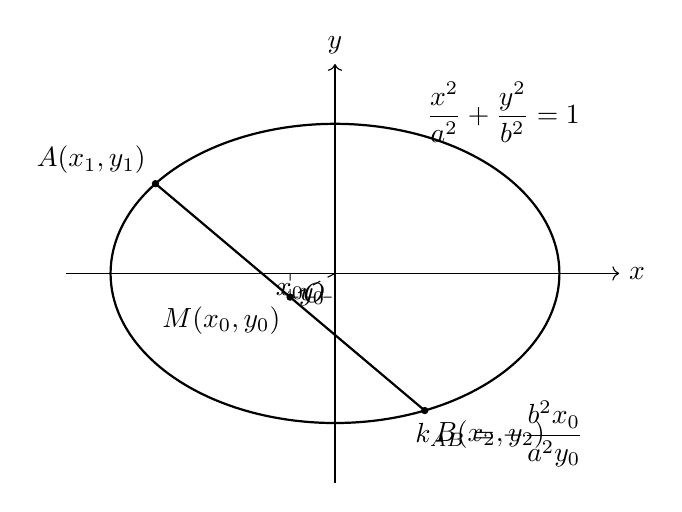
\begin{tikzpicture}[scale=0.95]
  \draw[->] (-3.6,0) -- (3.8,0) node[right] {$x$};
  \draw[->] (0,-2.8) -- (0,2.8) node[above] {$y$};
  \draw (0,0) node[below left] {$O$};

  \draw[thick,domain=0:360,samples=200,smooth] plot ({3*cos(\x)},{2*sin(\x)});

  \coordinate (A) at (-2.4,1.2);
  \coordinate (B) at (1.2,-1.8333333333);
  \coordinate (M) at (-0.6,-0.3166666667);

  \draw[thick] (A) -- (B);
  \draw[dashed] (0,0) -- (M);

  \fill (A) circle (1.4pt) node[above left] {$A(x_1,y_1)$};
  \fill (B) circle (1.4pt) node[below right] {$B(x_2,y_2)$};
  \fill (M) circle (1.4pt) node[below left] {$M(x_0,y_0)$};

  \draw[dashed] (M) -- (-0.6,0) node[below] {$x_0$};
  \draw[dashed] (M) -- (0,-0.3166666667) node[left] {$y_0$};

  \node at (2.25,2.15) {$\displaystyle \frac{x^2}{a^2}+\frac{y^2}{b^2}=1$};
  \node at (2.2,-2.15) {$\displaystyle k_{AB}=-\frac{b^2x_0}{a^2y_0}$};
\end{tikzpicture}

\end{center}

\subsection*{对应高考真题}

\begin{gaokao}{2023 年高考数学 全国乙卷-理科第11题}

设 $A$，$B$ 为双曲线 $x^2-\frac{y^2}{9}=1$ 上两点，下列四个点中，可为线段 $AB$ 中点的是（ ）

\begin{enumerate}[label=\Alph*. ,itemsep=2pt]

\item $(1,1)$

\item $(-1,2)$

\item $(1,3)$

\item $(-1,-4)$

\end{enumerate}

\paragraph{技巧对应}

这题与本技巧的对应最直接、最典型。题目已知双曲线上的一条弦 $AB$，判断哪个点可以作为其中点。其标准解正是先设中点为 $M\bigl(\frac{x_1+x_2}{2},\frac{y_1+y_2}{2}\bigr)$，再对双曲线
\[
x^2-\frac{y^2}{9}=1
\]
中两点坐标代入后的两个方程作差，得到
\[
(x_1^2-x_2^2)-\frac{y_1^2-y_2^2}{9}=0,
\]
进而把弦斜率与中点方向联系起来，即
\[
k_{AB}\cdot k_{OM}=9.
\]
这正对应原摘录中双曲线 $\dfrac{x^2}{a^2}-\dfrac{y^2}{b^2}=1$ 的结论
\[
k_{AB}k_{OM}=\frac{b^2}{a^2}.
\]
本题不是一般地“联立求交点”，而是把“中点”作为核心信息来处理，点差法是主方法而不是陪衬方法，因此最能体现该技巧。

\paragraph{答案}

$(-1,-4)$

\paragraph{解答}

设 $A(x_1,y_1),B(x_2,y_2)$，则 $AB$ 的中点 $M(\frac{x_1+x_2}{2},\frac{y_1+y_2}{2})$，可得 $k_{AB}=\frac{y_1-y_2}{x_1-x_2}$，$k=\frac{\frac{y_1+y_2}{2}}{\frac{x_1+x_2}{2}}=\frac{y_1+y_2}{x_1+x_2}$，因为 $A,B$ 在双曲线上，则 $\begin{cases} x_1^2-\frac{y_1^2}{9}=1 \\ x_2^2-\frac{y_2^2}{9}=1 \end{cases}$，两式相减得 $(x_1^2-x_2^2)-\frac{y_1^2-y_2^2}{9}=0$，所以 $k_{AB}\cdot k=\frac{y_1^2-y_2^2}{x_1^2-x_2^2}=9$. 对于选项A：可得 $k=1$，$k_{AB}=9$，则 $AB:y=9x-8$，联立方程 $\begin{cases} y=9x-8 \\ x^2-\frac{y^2}{9}=1 \end{cases}$，消去 $y$ 得 $72x^2-2\times72x+73=0$，此时 $\Delta=(-2\times72)^2-4\times72\times73=-288<0$，所以直线 $AB$ 与双曲线没有交点，故A错误；对于选项B：可得 $k=-2$，$k_{AB}=-\frac{9}{2}$，则 $AB:y=-\frac{9}{2}x-\frac{5}{2}$，联立方程 $\begin{cases} y=-\frac{9}{2}x-\frac{5}{2} \\ x^2-\frac{y^2}{9}=1 \end{cases}$，消去 $y$ 得 $45x^2+2\times45x+61=0$，此时 $\Delta=(2\times45)^2-4\times45\times61=-4\times45\times16<0$，所以直线 $AB$ 与双曲线没有交点，故B错误；对于选项C：可得 $k=3$，$k_{AB}=3$，则 $AB:y=3x$，由双曲线方程可得 $a=1,b=3$，则 $AB:y=3x$ 为双曲线的渐近线，所以直线 $AB$ 与双曲线没有交点，故C错误；对于选项D：$k=4$，$k_{AB}=\frac{9}{4}$，则 $AB:y=\frac{9}{4}x-\frac{7}{4}$，联立方程 $\begin{cases} y=\frac{9}{4}x-\frac{7}{4} \\ x^2-\frac{y^2}{9}=1 \end{cases}$，消去 $y$ 得 $63x^2+126x-193=0$，此时 $\Delta=126^2+4\times63\times193>0$，故直线 $AB$ 与双曲线有两个交点，故D正确.

\par\smallskip\textcolor{gray}{\footnotesize 来源记录：\texttt{\detokenize{tex版(exam-zh模板2016-2025)/2023/2023-全国乙卷-理科/questions.json}}}

\end{gaokao}

\begin{gaokao}{2016 年高考数学 全国III卷-文科第20题}

已知抛物线 $C: y^2=2x$ 的焦点为 $F$, 平行于 $x$ 轴的两条直线 $l_1$, $l_2$ 分别交 $C$ 于 $A$, $B$ 两点, 交 $C$ 的准线于 $P$, $Q$ 两点.
(I) 若 $F$ 在线段 $AB$ 上, $R$ 是 $PQ$ 的中点, 证明 $AR\parallel FQ$;
(II) 若 $\triangle PQF$ 的面积是 $\triangle ABF$ 的面积的两倍, 求 $AB$ 中点的轨迹方程.

\begin{center}

\begin{tikzpicture}[scale=1.0]
  \draw[->] (-1.2,0) -- (4.8,0) node[right] {$x$};
  \draw[->] (0,-2.4) -- (0,2.8) node[above] {$y$};
  \draw (0,0) node[below left] {$O$};

  \draw[thick,domain=-2.1:2.1,samples=200,smooth] plot ({0.5*(\x)^2},{\x});
  \draw[dashed] (-0.7,0) -- (-0.7,2.4) node[above] {准线 $x=-\frac12$};

  \coordinate (A) at (0.5,1.0);
  \coordinate (B) at (4.5,-3.0);
  \coordinate (M) at (2.5,-1.0);
  \coordinate (N) at (1.0,0.0);
  \coordinate (F) at (0.5,0.0);
  \coordinate (P) at (-0.5,1.0);
  \coordinate (Q) at (-0.5,-3.0);

  \draw[thick] (A) -- (B);
  \draw[dashed] (P) -- (Q);
  \draw[dashed] (F) -- (Q);

  \fill (A) circle (1.2pt) node[above right] {$A$};
  \fill (B) circle (1.2pt) node[below right] {$B$};
  \fill (M) circle (1.2pt) node[below] {$M$};
  \fill (N) circle (1.2pt) node[above] {$N$};
  \fill (F) circle (1.2pt) node[below] {$F$};
  \fill (P) circle (1.2pt) node[left] {$P$};
  \fill (Q) circle (1.2pt) node[left] {$Q$};
\end{tikzpicture}

\end{center}

\paragraph{技巧对应}

本题第（II）问虽然表述为“求 $AB$ 中点的轨迹方程”，但核心步骤仍然是标准的点差法。设 $A(x_1,y_1),B(x_2,y_2)$ 在抛物线 $y^2=2x$ 上，由
\[
y_1^2=2x_1,\qquad y_2^2=2x_2
\]
作差得
\[
(y_1-y_2)(y_1+y_2)=2(x_1-x_2).
\]
再结合中点 $M(x,y)$ 满足
\[
y_1+y_2=2y,
\]
以及直线 $AB$ 经过定点时带来的斜率关系，便可推出中点轨迹。这与本技巧“由两点在曲线上，作差后把 $(x_1+x_2),(y_1+y_2)$ 换成中点坐标”的操作完全一致。

更重要的是，这题展示了点差法的另一类典型用途：不仅能由中点求弦方程，还能反过来研究一族弦的中点轨迹。这正好补充了原摘录中的“中点弦问题的应用场景”。

\paragraph{答案}

见解析

\paragraph{解答}

(I) 连接 $RF$, $PF$. 由 $AP=AF$, $BQ=BF$ 及 $AP\parallel BQ$, 得 $\angle AFP+\angle BFQ=90^{\circ}$, 所以 $\angle PFQ=90^{\circ}$. 因为 $R$ 是 $PQ$ 的中点, 所以 $RF=RP=RQ$, 所以 $\triangle PAR\cong\triangle FAR$, 所以 $\angle PAR=\angle FAR$, $\angle PRA=\angle FRA$. 又 $\angle BQF+\angle BFQ=180^{\circ}-\angle QBF=\angle PAF=2\angle PAR$, 所以 $\angle FQB=\angle PAR$, 所以 $\angle PRA=\angle PQF$, 所以 $AR\parallel FQ$.
(II) 设 $A(x_1,y_1)$, $B(x_2,y_2)$, $F(\frac{1}{2},0)$, 准线为 $x=-\frac{1}{2}$. $S_{\triangle PQF}=\frac{1}{2}|PQ|=\frac{1}{2}|y_1-y_2|$. 设直线 $AB$ 与 $x$ 轴交点为 $N$, 则 $S_{\triangle ABF}=\frac{1}{2}|FN||y_1-y_2|$. 因为 $\triangle PQF$ 的面积是 $\triangle ABF$ 的面积的两倍, 所以 $2|FN|=1$, 得 $x_N=1$, 即 $N(1,0)$. 设 $AB$ 中点为 $M(x,y)$, 由 $\begin{cases}y_1^2=2x_1\\ y_2^2=2x_2\end{cases}$ 得 $(y_1-y_2)(y_1+y_2)=2(x_1-x_2)$, 又 $\dfrac{y_1-y_2}{x_1-x_2}=\dfrac{y}{x-1}$, 所以 $y\cdot2y=2$, 即 $y^2=x-1$. 所以 $AB$ 中点轨迹方程为 $y^2=x-1$.

\par\smallskip\textcolor{gray}{\footnotesize 来源记录：\texttt{\detokenize{tex版(exam-zh模板2016-2025)/2016/2016-全国III卷-文科/questions.json}}}

\end{gaokao}

\clearpage

\section{技巧50：焦点三角形面积问题}

\subsection*{核心认识}

焦点三角形面积问题，指以圆锥曲线的焦点与曲线上一点构成的三角形面积问题。对椭圆、双曲线，常见图形是$\triangle PF_1F_2$；对抛物线，常见图形是过焦点的弦$AB$与顶点（或原点）构成的三角形。

这类问题的核心，不是先硬算点坐标，而是优先调用圆锥曲线定义与三角形面积公式。

对于椭圆$\dfrac{x^2}{a^2}+\dfrac{y^2}{b^2}=1\,(a>b>0)$，若$P$在椭圆上，$F_1,F_2$为焦点，$\angle F_1PF_2=\theta$，则
\[
|PF_1|+|PF_2|=2a,
\qquad
S_{\triangle PF_1F_2}=\frac12|PF_1|\,|PF_2|\sin\theta.
\]
进一步可推出
\[
|PF_1|\,|PF_2|=\frac{2b^2}{1+\cos\theta},
\qquad
S_{\triangle PF_1F_2}=b^2\tan\frac{\theta}{2}.
\]

对于双曲线$\dfrac{x^2}{a^2}-\dfrac{y^2}{b^2}=1$，若$P$在双曲线上，$F_1,F_2$为焦点，$\angle F_1PF_2=\theta$，则
\[
\bigl||PF_1|-|PF_2|\bigr|=2a,
\qquad
S_{\triangle PF_1F_2}=\frac12|PF_1|\,|PF_2|\sin\theta.
\]
进一步可推出
\[
|PF_1|\,|PF_2|=\frac{2b^2}{1-\cos\theta},
\qquad
S_{\triangle PF_1F_2}=\frac{b^2}{\tan\dfrac{\theta}{2}}.
\]

对于抛物线$y^2=2px\,(p>0)$，过焦点$F$的直线交抛物线于$A,B$两点，$O$为原点，若该直线倾斜角为$\theta\in(0,\pi)$，则$\triangle OAB$是等腰三角形，且
\[
S_{\triangle OAB}=\frac{p^2}{2\sin\theta}.
\]

因此，遇到焦点三角形面积时，应先判断是椭圆、双曲线还是抛物线，再看题目给的是角、边长关系、垂直关系，还是坐标与弦的条件，选择对应公式或由定义配合余弦定理求解。

\subsection*{操作步骤}

\begin{enumerate}

\item 先辨认图形是否为焦点三角形：椭圆、双曲线中通常是$\triangle PF_1F_2$，抛物线中通常是过焦点的弦与顶点构成的三角形

\item 先写出圆锥曲线定义：椭圆用$|PF_1|+|PF_2|=2a$，双曲线用$\bigl||PF_1|-|PF_2|\bigr|=2a$，抛物线优先利用焦点弦性质

\item 若已知$\angle F_1PF_2=\theta$，直接考虑面积公式$S=\dfrac12|PF_1|\,|PF_2|\sin\theta$

\item 椭圆中若已知顶角$\theta$，可直接用$S=b^2\tan\dfrac{\theta}{2}$；双曲线中若已知顶角$\theta$，可直接用$S=\dfrac{b^2}{\tan\dfrac{\theta}{2}}$

\item 若题目给出垂直关系，如$PF_1\perp PF_2$，则先化为$\angle F_1PF_2=90^\circ$，再把面积公式大幅简化

\item 若题目给出原点到点$P$的距离、斜率、数量积等条件，可先转化出角或边的关系，再回到焦点三角形面积

\item 当直接公式不能一步得到结果时，用余弦定理把$|F_1F_2|,|PF_1|,|PF_2|,\angle F_1PF_2$联系起来，再配合定义求面积

\item 计算结束后，注意核对所求到底是三角形面积、四边形面积，还是由面积反求参数

\end{enumerate}

\subsection*{结构图}

\begin{center}

\begin{tikzpicture}[scale=1.0]
  \coordinate (F1) at (-2.2,0);
  \coordinate (F2) at (2.2,0);
  \coordinate (P1) at (0,2.1);
  \coordinate (P2) at (0,2.6);

  \draw[thick] (0,0) ellipse (3 and 2);
  \draw[thick] (0,0) plot[domain=-3.2:-1.21,smooth,variable=\x] ({\x},{sqrt(0.75*(\x*\x-1.44))});
  \draw[thick] (0,0) plot[domain=-3.2:-1.21,smooth,variable=\x] ({\x},{-sqrt(0.75*(\x*\x-1.44))});
  \draw[thick] (0,0) plot[domain=1.21:3.2,smooth,variable=\x] ({\x},{sqrt(0.75*(\x*\x-1.44))});
  \draw[thick] (0,0) plot[domain=1.21:3.2,smooth,variable=\x] ({\x},{-sqrt(0.75*(\x*\x-1.44))});

  \draw[dashed] (F1)--(F2);
  \draw[blue,thick] (P1)--(F1)--(F2)--cycle;
  \draw[red,thick] (P2)--(F1)--(F2)--cycle;

  \fill (F1) circle (1.4pt) node[below] {$F_1$};
  \fill (F2) circle (1.4pt) node[below] {$F_2$};
  \fill (P1) circle (1.4pt) node[above right] {$P$};
  \fill (P2) circle (1.4pt) node[above right] {$P$};

  \node at (0,-2.35) {椭圆中$S_{\triangle PF_1F_2}=b^2\tan\dfrac{\theta}{2}$};
  \node at (0,3.05) {双曲线中$S_{\triangle PF_1F_2}=\dfrac{b^2}{\tan\dfrac{\theta}{2}}$};
\end{tikzpicture}

\end{center}

\subsection*{对应高考真题}

\begin{gaokao}{2020 年高考数学 全国I卷-文科第11题}

设 $F_1, F_2$ 是双曲线 $C: x^2 - \frac{y^2}{3} = 1$ 的两个焦点，$O$ 为坐标原点，点 $P$ 在 $C$ 上且 $|OP| = 2$, 则 $\triangle PF_1F_2$ 的面积为

\begin{enumerate}[label=\Alph*. ,itemsep=2pt]

\item $\frac{7}{2}$

\item $3$

\item $\frac{5}{2}$

\item $2$

\end{enumerate}

\paragraph{技巧对应}

这道题与本技巧的对应最直接。题目所求正是双曲线焦点三角形$\triangle PF_1F_2$的面积，且解答过程本质上围绕焦点三角形展开：由$|OP|=2=\dfrac12|F_1F_2|$先判定$\angle F_1PF_2=90^\circ$，再结合双曲线定义$|PF_1|-|PF_2|=2a$求出$|PF_1|\,|PF_2|$，最后用
\[
S_{\triangle PF_1F_2}=\frac12|PF_1|\,|PF_2|
\]
得到面积。它完整体现了“焦点三角形面积问题”的标准做法：先找角，再用定义与边角关系算面积。

\paragraph{答案}

$3$

\paragraph{解答}

由已知，$F_1(-2,0), F_2(2,0)$, 则 $a=1, c=2$, 因为 $|OP|=2 = \frac{1}{2}|F_1F_2|$, 所以点 $P$ 在以 $F_1F_2$ 为直径的圆上，即 $\triangle PF_1F_2$ 是以 $P$ 为直角顶点的直角三角形，故 $|PF_1|^2 + |PF_2|^2 = |F_1F_2|^2 = 16$, 又 $|PF_1|-|PF_2|=2a=2$, 所以 $4 = (|PF_1|-|PF_2|)^2 = |PF_1|^2 + |PF_2|^2 - 2|PF_1||PF_2| = 16 - 2|PF_1||PF_2|$, 解得 $|PF_1||PF_2|=6$, 所以 $S_{\triangle PF_1F_2} = \frac{1}{2}|PF_1||PF_2|=3$.

\par\smallskip\textcolor{gray}{\footnotesize 来源记录：\texttt{\detokenize{tex版(exam-zh模板2016-2025)/2020/2020-全国I卷-文科/questions.json}}}

\end{gaokao}

\begin{gaokao}{2023 年高考数学 全国甲卷-理科第12题}

设 $O$ 为坐标原点，$F_1$，$F_2$ 为椭圆 $C: \frac{x^2}{9} + \frac{y^2}{6} = 1$ 的两个焦点，点 $P$ 在 $C$ 上，$\cos\angle F_1PF_2 = \frac{3}{5}$，则 $|OP| = $（         ）

\begin{enumerate}[label=\Alph*. ,itemsep=2pt]

\item $\frac{\sqrt{13}}{5}$

\item $\frac{\sqrt{30}}{2}$

\item $\frac{\sqrt{14}}{5}$

\item $\frac{\sqrt{35}}{2}$

\end{enumerate}

\paragraph{技巧对应}

这道题高度体现了椭圆焦点三角形面积公式的应用价值。题设直接给出$\cos\angle F_1PF_2=\dfrac35$，而本技巧中椭圆情形的核心结论正是
\[
S_{\triangle PF_1F_2}=b^2\tan\frac{\theta}{2}.
\]
解答中先由$\cos\angle F_1PF_2$转化出$\tan\dfrac{\theta}{2}$，再迅速得到焦点三角形面积，继而反求点$P$的纵坐标，最终求出$|OP|$。这说明焦点三角形面积公式不仅能直接求面积，还能作为中间量服务于后续求点的位置或距离，是本技巧的典型延伸应用。

\paragraph{答案}

B

\paragraph{解答}

方法一：设 $\angle F_1PF_2 = 2\theta$，$0<\theta<\frac{\pi}{2}$，所以 $S_{\triangle PF_1F_2} = b^2\tan\frac{\angle F_1PF_2}{2} = b^2\tan\theta$，由 $\cos\angle F_1PF_2 = \cos2\theta = \frac{\cos^2\theta-\sin^2\theta}{\cos^2\theta+\sin^2\theta} = \frac{1-\tan^2\theta}{1+\tan^2\theta} = \frac{3}{5}$，解得：$\tan\theta = \frac{1}{2}$，由椭圆方程可知，$a^2=9$，$b^2=6$，$c^2=a^2-b^2=3$，所以 $S_{\triangle PF_1F_2} = \frac{1}{2}\times F_1F_2\times|y_p| = \frac{1}{2}\times2\sqrt{3}\times|y_p| = 6\times\frac{1}{2}$，解得：$y_p^2=3$，则 $x_p^2 = 9\times\left(1-\frac{3}{6}\right) = \frac{9}{2}$，因此 $|OP| = \sqrt{x_p^2+y_p^2} = \sqrt{3+\frac{9}{2}} = \frac{\sqrt{30}}{2}$．故选：B．
方法二：因为 $|PF_1|+|PF_2|=2a=6$ (1)，$|PF_1|^2+|PF_2|^2-2|PF_1||PF_2|\cos\angle F_1PF_2 = |F_1F_2|^2$，即 $|PF_1|^2+|PF_2|^2 - \frac{6}{5}|PF_1||PF_2| = 12$ (2)，联立(1)(2)，解得：$|PF_1||PF_2| = \frac{15}{2}$，$|PF_1|^2+|PF_2|^2 = 21$，而 $\overrightarrow{PO} = \frac{1}{2}(\overrightarrow{PF_1}+\overrightarrow{PF_2})$，所以 $|\overrightarrow{OP}| = |\overrightarrow{PO}| = \frac{1}{2}\sqrt{|\overrightarrow{PF_1}|^2+|\overrightarrow{PF_2}|^2+2\overrightarrow{PF_1}\cdot\overrightarrow{PF_2}} = \frac{1}{2}\sqrt{21+2\times\frac{3}{5}\times\frac{15}{2}} = \frac{\sqrt{30}}{2}$．故选：B．
方法三：因为 $|PF_1|+|PF_2|=2a=6$ (1)，$|PF_1|^2+|PF_2|^2-2|PF_1||PF_2|\cos\angle F_1PF_2 = |F_1F_2|^2$，即 $|PF_1|^2+|PF_2|^2 - \frac{6}{5}|PF_1||PF_2| = 12$ (2)，联立(1)(2)，解得：$|PF_1|^2+|PF_2|^2 = 21$，由中线定理可知，$2(|OP|^2+|OF_1|^2) = |PF_1|^2+|PF_2|^2 = 42$，易知 $|F_1F_2| = 2\sqrt{3}$，解得：$|OP| = \frac{\sqrt{30}}{2}$．故选：B．

\par\smallskip\textcolor{gray}{\footnotesize 来源记录：\texttt{\detokenize{tex版(exam-zh模板2016-2025)/2023/2023-全国甲卷-理科/questions.json}}}

\end{gaokao}

\begin{gaokao}{2020 年高考数学 全国III卷-理科第11题}

设双曲线 $C:\dfrac{x^2}{a^2}-\dfrac{y^2}{b^2}=1\ (a>0,b>0)$ 的左、右焦点分别为 $F_1,F_2$，离心率为 $\sqrt{5}$。$P$ 是 $C$ 上一点，且 $F_1P\perp F_2P$。若 $\triangle PF_1F_2$ 的面积为 $4$，则 $a=$

\begin{enumerate}[label=\Alph*. ,itemsep=2pt]

\item $1$

\item $2$

\item $4$

\item $8$

\end{enumerate}

\paragraph{技巧对应}

这道题与双曲线焦点三角形面积技巧具有实质对应。题目已知$F_1P\perp F_2P$，这等价于焦点三角形$\triangle PF_1F_2$在$P$处为直角三角形，于是面积满足
\[
S_{\triangle PF_1F_2}=\frac12|PF_1|\,|PF_2|.
\]
再结合双曲线定义$|PF_1|-|PF_2|=2a$以及勾股关系$|PF_1|^2+|PF_2|^2=(2c)^2$，即可由面积反推出参数$a$。它体现了本技巧中“由垂直条件先把焦点三角形特殊化，再借定义求参数”的常见路径。

\paragraph{答案}

$A$

\paragraph{解答}

因为 $e=\dfrac{c}{a}=\sqrt{5}$，所以 $c=\sqrt{5}a$。根据双曲线定义 $|PF_1|-|PF_2|=2a$。$\triangle PF_1F_2$ 面积 $\dfrac12|PF_1|\cdot|PF_2|=4$，得 $|PF_1|\cdot|PF_2|=8$。又 $F_1P\perp F_2P$，所以 $|PF_1|^2+|PF_2|^2=(2c)^2=20a^2$。而 $(|PF_1|-|PF_2|)^2=4a^2$，即 $|PF_1|^2+|PF_2|^2-2|PF_1|\cdot|PF_2|=4a^2$，所以 $20a^2-16=4a^2$，得 $16a^2=16$，$a=1$。故选 $A$。

\par\smallskip\textcolor{gray}{\footnotesize 来源记录：\texttt{\detokenize{tex版(exam-zh模板2016-2025)/2020/2020-全国III卷-理科/questions.json}}}

\end{gaokao}

\clearpage

\section{技巧51：焦点弦长问题}

\subsection*{核心认识}

若圆锥曲线的一条弦所在直线经过焦点，这条弦叫做焦点弦。此类问题的关键，不是先把交点坐标硬算出来，而是优先识别“过焦点”“给倾斜角或斜率”“求弦长、焦半径、最值”这些信号，然后直接调用焦点弦的长度关系。

对直线 $y=kx+m$ 与圆锥曲线交于 $A(x_1,y_1),B(x_2,y_2)$，总有
\[
|AB|=\sqrt{1+k^2}\,|x_1-x_2|
\]
或在 $k\ne 0$ 时
\[
|AB|=\sqrt{1+\frac1{k^2}}\,|y_1-y_2|.
\]
这只是一般弦长公式；若它还是焦点弦，就能进一步化简。

椭圆 $\dfrac{x^2}{a^2}+\dfrac{y^2}{b^2}=1\,(a>b>0)$ 中，设焦点弦 $AB$ 过右焦点 $F(c,0)$，其倾斜角为 $\alpha$，则
\[
|AF|=\frac{b^2}{a+c\cos\alpha},\qquad |BF|=\frac{b^2}{a-c\cos\alpha},
\]
\[
|AB|=\frac{2ab^2}{a^2-c^2\cos^2\alpha}.
\]
特别地，当弦垂直于长轴时，它是通径，
\[
|AB|=\frac{2b^2}{a}.
\]

抛物线 $y^2=2px\,(p>0)$ 中，若焦点弦 $MN$ 的倾斜角为 $\alpha$，则
\[
|MN|=\frac{2p}{\sin^2\alpha},
\]
并且若 $M(x_1,y_1),N(x_2,y_2)$，还有
\[
|MN|=x_1+x_2+p.
\]
因此：已知焦点、方向角、通径位置或两端点与焦点的数量关系时，应优先用焦点弦公式；只有在条件不足时，再回到联立方程与根系关系。

\subsection*{操作步骤}

\begin{enumerate}

\item \item 先判断所求弦是否经过焦点；若是，就把题目归入焦点弦问题。

\item \item 再看已知条件属于哪一类：给倾斜角（或斜率）、给通径、给焦半径和、给弦长最值，分别对应不同的焦点弦结论。

\item \item 椭圆或双曲线中，若已知焦点弦的倾斜角，优先使用 $|AB|$ 关于 $a,b,c,\alpha$ 的公式；不要急于联立直线与曲线方程。

\item \item 抛物线中，若直线过焦点，优先考虑 $|MN|=\dfrac{2p}{\sin^2\alpha}$ 或 $|MN|=x_1+x_2+p$；这通常比设点、消元更快。

\item \item 若题目给的是斜率而不是倾斜角，先由 $k=\tan\alpha$ 转成三角量，再代入焦点弦公式。

\item \item 若题目只给出交点坐标和直线斜率，可先用一般弦长公式 $|AB|=\sqrt{1+k^2}\,|x_1-x_2|$，再结合根与系数关系化简。

\item \item 求最值时，焦点弦公式往往会把问题化成关于 $\sin^2\alpha$ 或 $\cos^2\alpha$ 的最值，这一步通常比坐标法更直接。

\item \item 算完后要检查图形位置：如双曲线要分同支、异支两种情形；抛物线要注意倾斜角不能使直线与对称轴平行到不成弦。

\end{enumerate}

\subsection*{结构图}

\begin{center}

\begin{tikzpicture}[scale=1.05]
  \draw[->] (-3.6,0) -- (3.8,0) node[right] {$x$};
  \draw[->] (0,-2.5) -- (0,2.7) node[above] {$y$};
  \def\a{3}
  \def\b{2}
  \def\c{2.2360679}
  \draw[smooth,domain=0:360,samples=200] plot ({\a*cos(\x)},{\b*sin(\x)});
  \fill (\c,0) circle (1.2pt) node[below right] {$F$};
  \fill (-\c,0) circle (1.2pt);
  \draw[dashed] (\c,0) -- ++(35:2.8);
  \draw[name path=line] (-0.4,-1.85) -- (3.5,0.88);
  \fill (0.122,-1.484) circle (1.2pt) node[below] {$A$};
  \fill (2.958,0.501) circle (1.2pt) node[above right] {$B$};
  \draw (0.122,-1.484) -- (2.958,0.501);
  \draw (\c+0.42,0) arc[start angle=0,end angle=35,radius=0.42];
  \node at (2.9,0.22) {$\alpha$};
  \node at (1.55,1.95) {$\displaystyle \frac{x^2}{a^2}+\frac{y^2}{b^2}=1$};
  \node at (1.55,-2.1) {过焦点的弦 $AB$};
\end{tikzpicture}

\end{center}

\subsection*{对应高考真题}

\begin{gaokao}{2017 年高考数学 全国I卷-理科第10题}

已知 $F$ 为抛物线 $C:y^2=4x$ 的焦点，过 $F$ 作两条互相垂直的直线 $l_1$，$l_2$，直线 $l_1$ 与 $C$ 交于 $A$、$B$ 两点，直线 $l_2$ 与 $C$ 交于 $D$、$E$ 两点，则 $|AB|+|DE|$ 的最小值为（ ）

\begin{enumerate}[label=\Alph*. ,itemsep=2pt]

\item $16$

\item $14$

\item $12$

\item $10$

\end{enumerate}

\begin{center}

\begin{tikzpicture}[scale=1.0]
  \draw[->] (-1.8,0) -- (5.2,0) node[right] {$x$};
  \draw[->] (0,-3.2) -- (0,3.2) node[above] {$y$};
  \draw[smooth,domain=-3.1:3.1,samples=200] plot ({(\x*\x)/4},{\x});
  \fill (1,0) circle (1.2pt) node[below] {$F$};
  \draw (-0.4,-1.4) -- (3.9,2.9) node[right] {$l_2$};
  \draw (-0.4,1.4) -- (3.9,-2.9) node[right] {$l_1$};
  \fill (2.914,1.914) circle (1.2pt) node[above right] {$D$};
  \fill (0.086,-0.914) circle (1.2pt) node[below left] {$E$};
  \fill (2.914,-1.914) circle (1.2pt) node[below right] {$A$};
  \fill (0.086,0.914) circle (1.2pt) node[above left] {$B$};
\end{tikzpicture}

\end{center}

\paragraph{技巧对应}

这题与本技巧对应最直接。题设明确给出“过抛物线焦点作两条互相垂直的直线”，两条截得的都是焦点弦，所求又是 $|AB|+|DE|$ 的最小值。其标准解法正是把两条弦长写成
\[
|AB|=\frac{2p}{\sin^2\theta},\qquad |DE|=\frac{2p}{\cos^2\theta}
\]
再转化为三角最值问题。这充分体现了焦点弦长公式在“过焦点+给方向关系+求长度最值”中的优势。

\paragraph{答案}

A

\paragraph{解答}

方法一：如图，$l_1\perp l_2$，要使 $|AB|+|DE|$ 最小，则 $A$ 与 $D$，$B$，$E$ 关于 $x$ 轴对称，即直线 $DE$ 的斜率为 1，又直线 $l_2$ 过点 $(1,0)$，则直线 $l_2$ 的方程为 $y=x-1$，联立 $\begin{cases} y^2=4x \\ y=x-1 \end{cases}$，则 $y^2-4y-4=0$，\ensuremath{\therefore}$y_1+y_2=4$，$y_1y_2=-4$，\ensuremath{\therefore}$|DE|=\sqrt{1+1^2}\cdot|y_1-y_2|=\sqrt{2}\times\sqrt{4^2+16}=8$，\ensuremath{\therefore}$|AB|+|DE|$ 的最小值为 $2|DE|=16$．方法二：设直线 $l_1$ 的倾斜角为 $\theta$，则 $l_2$ 的倾斜角为 $\frac{\pi}{2}+\theta$，根据焦点弦长公式可得 $|AB|=\frac{2p}{\sin^2\theta}=\frac{4}{\sin^2\theta}$，$|DE|=\frac{4}{\sin^2(\frac{\pi}{2}+\theta)}=\frac{4}{\cos^2\theta}$，\ensuremath{\therefore}$|AB|+|DE|=\frac{4}{\sin^2\theta}+\frac{4}{\cos^2\theta}=\frac{4}{\sin^2\theta\cos^2\theta}=\frac{16}{\sin^2 2\theta}$，\ensuremath{\because}$0<\sin^2 2\theta\leq 1$，\ensuremath{\therefore}当 $\theta=45^\circ$ 时，$|AB|+|DE|$ 最小，最小为 16．故选：A．

\par\smallskip\textcolor{gray}{\footnotesize 来源记录：\texttt{\detokenize{tex版(exam-zh模板2016-2025)/2017/2017-全国I卷-理科/questions.json}}}

\end{gaokao}

\begin{gaokao}{2023 年高考数学 新高考II卷第10题}

设$O$为坐标原点，直线$y=-\sqrt{3}(x-1)$过抛物线$C:y^{2}=2px(p>0)$的焦点，且与$C$交于$M$，$N$两点，$l$为$C$的准线，则（ \quad ）

\begin{enumerate}[label=\Alph*. ,itemsep=2pt]

\item A. $p=2$

\item B. $|MN|=\dfrac{8}{3}$

\item C. 以$MN$为直径的圆与$l$相切

\item D. $\triangle OMN$为等腰三角形

\end{enumerate}

\begin{center}

\begin{tikzpicture}[scale=1.0]
  \draw[->] (-1.8,0) -- (5.2,0) node[right] {$x$};
  \draw[->] (0,-3.2) -- (0,3.2) node[above] {$y$};
  \draw[smooth,domain=-3.1:3.1,samples=200] plot ({(\x*\x)/4},{\x});
  \draw[dashed] (-1,-3.0) -- (-1,3.0) node[above] {$l$};
  \fill (1,0) circle (1.2pt) node[below] {$F$};
  \draw (-0.3,2.25) -- (3.7,-0.06);
  \fill (3,-1.732) circle (1.2pt) node[below right] {$M$};
  \fill (0.333,0.577) circle (1.2pt) node[above left] {$N$};
\end{tikzpicture}

\end{center}

\paragraph{技巧对应}

这题也是典型焦点弦题。直线 $y=-\sqrt{3}(x-1)$ 过抛物线 $C:y^2=2px$ 的焦点，并与抛物线交于 $M,N$ 两点，所以 $MN$ 就是焦点弦。选项 B 直接考查 $|MN|$，可由抛物线焦点弦长公式快速得到；选项 C 又利用了焦点弦与准线之间的几何关系。因此本题不仅考查“会算焦点弦长”，还考查“会用焦点弦的几何结构”。

\paragraph{答案}

AC

\paragraph{解答}

A选项：直线$y=-\sqrt{3}(x-1)$过点$(1,0)$，所以抛物线$C:y^{2}=2px(p>0)$的焦点$F(1,0)$，所以$\dfrac{p}{2}=1$，$p=2$，$2p=4$，则A正确，且抛物线$C$的方程为$y^{2}=4x$.
B选项：设$M(x_{1},y_{1})$，$N(x_{2},y_{2})$，由$\begin{cases}y=-\sqrt{3}(x-1)\\ y^{2}=4x\end{cases}$消去$y$并化简得$3x^{2}-10x+3=(x-3)(3x-1)=0$，解得$x_{1}=3$，$x_{2}=\dfrac{1}{3}$，所以$|MN|=x_{1}+x_{2}+p=3+\dfrac{1}{3}+2=\dfrac{16}{3}$，B错误.
C选项：设$MN$的中点为$A$，$M,N,A$到直线$l$的距离分别为$d_{1},d_{2},d$，因为$d=\dfrac{1}{2}(d_{1}+d_{2})=\dfrac{1}{2}(|MF|+|NF|)=\dfrac{1}{2}|MN|$，即$A$到直线$l$的距离等于$|MN|$的一半，所以以$MN$为直径的圆与直线$l$相切，C正确.
D选项：直线$y=-\sqrt{3}(x-1)$即$\sqrt{3}x+y-\sqrt{3}=0$，$O$到直线的距离为$d=\dfrac{\sqrt{3}}{2}$，所以三角形$OMN$的面积为$\dfrac{1}{2}\times\dfrac{16}{3}\times\dfrac{\sqrt{3}}{2}=\dfrac{4\sqrt{3}}{3}$，由上述分析可知$y_{1}=-\sqrt{3}(3-1)=-2\sqrt{3}$，$y_{2}=-\sqrt{3}\left(\dfrac{1}{3}-1\right)=\dfrac{2\sqrt{3}}{3}$，所以$|OM|=\sqrt{3^{2}+(-2\sqrt{3})^{2}}=\sqrt{21}$，$|ON|=\sqrt{\left(\dfrac{1}{3}\right)^{2}+\left(\dfrac{2\sqrt{3}}{3}\right)^{2}}=\dfrac{\sqrt{13}}{3}$，所以三角形$OMN$不是等腰三角形，D错误.

\par\smallskip\textcolor{gray}{\footnotesize 来源记录：\texttt{\detokenize{tex版(exam-zh模板2016-2025)/2023/2023-新高考II卷/questions.json}}}

\end{gaokao}

\begin{gaokao}{2020 年高考数学 全国II卷-理科第19题}

已知椭圆$C_1:\dfrac{x^2}{a^2}+\dfrac{y^2}{b^2}=1(a>b>0)$的右焦点$F$与抛物线$C_2$的焦点重合，$C_1$的中心与$C_2$的顶点重合.过$F$且与$x$轴垂直的直线交$C_1$于$A,B$两点，交$C_2$于$C,D$两点，且$|CD|=\dfrac43|AB|$.
（1）求$C_1$的离心率；
（2）设$M$是$C_1$与$C_2$的公共点，若$|MF|=5$，求$C_1$与$C_2$的标准方程.

\begin{center}

\begin{tikzpicture}[scale=0.95]
  \draw[->] (-4.2,0) -- (4.5,0) node[right] {$x$};
  \draw[->] (0,-3.2) -- (0,3.2) node[above] {$y$};
  \draw[smooth,domain=0:360,samples=200] plot ({3*cos(\x)},{2.2*sin(\x)});
  \draw[smooth,domain=-3.2:3.2,samples=200] plot ({(\x*\x)/4},{\x});
  \fill (1.5,0) circle (1.2pt) node[below] {$F$};
  \draw[dashed] (1.5,-3.0) -- (1.5,3.0);
  \fill (1.5,1.903) circle (1.2pt) node[right] {$A$};
  \fill (1.5,-1.903) circle (1.2pt) node[right] {$B$};
  \fill (1.5,2.449) circle (1.2pt) node[right] {$C$};
  \fill (1.5,-2.449) circle (1.2pt) node[right] {$D$};
  \node at (2.8,2.55) {$x=c$};
\end{tikzpicture}

\end{center}

\paragraph{技巧对应}

这题虽然是椭圆与抛物线综合题，但第（1）问中“过焦点且与 $x$ 轴垂直的直线交椭圆于 $A,B$ 两点”本质上就是椭圆的通径问题。解答中直接用到
\[
|AB|=\frac{2b^2}{a},
\]
这正是焦点弦长问题中最常用的特殊结论之一。它很好体现了“识别通径，绕开联立方程”的技巧价值。

\paragraph{答案}

（1）$\dfrac12$；（2）$C_1:\dfrac{x^2}{36}+\dfrac{y^2}{27}=1$，$C_2:y^2=12x$

\paragraph{解答}

（1）$\because F(c,0)$，$AB\perp x$轴且与椭圆$C_1$相交于$A,B$两点，则直线$AB$的方程为$x=c$，联立$\begin{cases}x=c\\\dfrac{x^2}{a^2}+\dfrac{y^2}{b^2}=1\end{cases}$，解得$y=\pm\dfrac{b^2}{a}$，则$|AB|=\dfrac{2b^2}{a}$，抛物线$C_2$的方程为$y^2=4cx$，联立$\begin{cases}x=c\\y^2=4cx\end{cases}$，解得$y=\pm2c$，$\therefore |CD|=4c$，$\because CD=\dfrac43AB$，即$4c=\dfrac43\times\dfrac{2b^2}{a}$，$\therefore 2b^2=3ac$，即$2(a^2-c^2)=3ac$，即$2c^2+3ac-2a^2=0$，即$2e^2+3e-2=0$，$\because 0<e<1$，解得$e=\dfrac12$.
（2）由（1）知$a=2c$，$b=\sqrt3c$，椭圆$C_1$的方程为$\dfrac{x^2}{4c^2}+\dfrac{y^2}{3c^2}=1$，联立$\begin{cases}y^2=4cx\\\dfrac{x^2}{4c^2}+\dfrac{y^2}{3c^2}=1\end{cases}$，消去$y$并整理得$3x^2+16cx-12c^2=0$，解得$x=\dfrac23c$或$x=-6c$（舍去），由抛物线的定义可得$|MF|=\dfrac23c+c=\dfrac{5c}{3}=5$，解得$c=3$，$\therefore$曲线$C_1$的标准方程为$\dfrac{x^2}{36}+\dfrac{y^2}{27}=1$，曲线$C_2$的标准方程为$y^2=12x$.

\par\smallskip\textcolor{gray}{\footnotesize 来源记录：\texttt{\detokenize{tex版(exam-zh模板2016-2025)/2020/2020-全国II卷-理科/questions.json}}}

\end{gaokao}

\clearpage

\section{技巧52：焦点三角形中的离心率求法}

\subsection*{核心认识}

设点 $P$ 在圆锥曲线上，$F_1,F_2$ 为焦点，则三角形 $PF_1F_2$ 常称为焦点三角形．这类问题的关键是把“离心率”转化为焦点三角形中的边角关系．

对椭圆 $\dfrac{x^2}{a^2}+\dfrac{y^2}{b^2}=1(a>b>0)$，若 $\angle PF_1F_2=\alpha,\ \angle PF_2F_1=\beta$，则
\[
e=\frac{c}{a}=\frac{|F_1F_2|}{|PF_1|+|PF_2|}
=\frac{\sin(\alpha+\beta)}{\sin\alpha+\sin\beta}
=\frac{\cos\dfrac{\alpha+\beta}{2}}{\cos\dfrac{\alpha-\beta}{2}}.
\]
其中 $\angle F_1PF_2=\pi-(\alpha+\beta)$，故上式中的 $\sin(\alpha+\beta)$ 也可理解为 $\sin\angle F_1PF_2$．

对双曲线 $\dfrac{x^2}{a^2}-\dfrac{y^2}{b^2}=1(a>0,b>0)$，若 $\angle PF_1F_2=\alpha,\ \angle PF_2F_1=\beta$，则
\[
e=\frac{c}{a}=\frac{|F_1F_2|}{\bigl||PF_1|-|PF_2|\bigr|}
=\left|\frac{\sin(\alpha+\beta)}{\sin\beta-\sin\alpha}\right|
=\left|\frac{\sin\dfrac{\alpha+\beta}{2}}{\sin\dfrac{\alpha-\beta}{2}}\right|.
\]

因此，已知焦点三角形的角，优先用正弦定理与椭圆、双曲线定义建立 $a,c$ 的关系，往往比坐标运算更直接．

\subsection*{操作步骤}

\begin{enumerate}

\item 先判断曲线类型：若是椭圆，用 $|PF_1|+|PF_2|=2a$；若是双曲线，用 $\bigl||PF_1|-|PF_2|\bigr|=2a$．

\item 在 $\triangle PF_1F_2$ 中设两底角分别为 $\alpha,\beta$，则顶角为 $\pi-(\alpha+\beta)$，从而 $\sin\angle F_1PF_2=\sin(\alpha+\beta)$．

\item 由正弦定理写出
\[
\frac{|PF_1|}{\sin\beta}=\frac{|PF_2|}{\sin\alpha}=\frac{|F_1F_2|}{\sin(\alpha+\beta)}.
\]
据此把 $|PF_1|,|PF_2|$ 都化成含 $|F_1F_2|$ 与角的式子．

\item 若求椭圆离心率，就把 $e=\dfrac{|F_1F_2|}{|PF_1|+|PF_2|}$ 代入化简；若求双曲线离心率，就把 $e=\dfrac{|F_1F_2|}{\bigl||PF_1|-|PF_2|\bigr|}$ 代入化简．

\item 若题目出现 $PF_1\perp PF_2$，则顶角为 $90^\circ$，有 $\alpha+\beta=90^\circ$，公式会进一步简化，这是高频切入点．

\item 若题目没有直接给出角，而给出等边、直角、面积、切线、圆等几何条件，应先把这些条件转化为焦点三角形中的边角关系，再套用上述思路．

\end{enumerate}

\subsection*{结构图}

\begin{center}

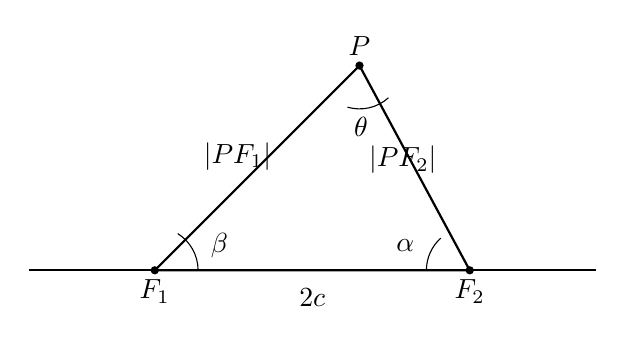
\begin{tikzpicture}[scale=1]
\coordinate (F1) at (-2,0);
\coordinate (F2) at (2,0);
\coordinate (P) at (0.6,2.6);
\draw[thick] (-3.6,0) -- (3.6,0);
\draw[thick] (F1) -- (P) -- (F2) -- cycle;
\fill (F1) circle (1.5pt) node[below] {$F_1$};
\fill (F2) circle (1.5pt) node[below] {$F_2$};
\fill (P) circle (1.5pt) node[above] {$P$};
\node at (0,-0.35) {$2c$};
\draw (F1)+(0.55,0) arc[start angle=0,end angle=58,radius=0.55];
\node at (-1.18,0.32) {$\beta$};
\draw (F2)+(-0.55,0) arc[start angle=180,end angle=132,radius=0.55];
\node at (1.18,0.32) {$\alpha$};
\draw (P)+(-106:0.55) arc[start angle=-106,end angle=-48,radius=0.55];
\node at (0.62,1.82) {$\theta$};
\node at (-0.95,1.45) {$|PF_1|$};
\node at (1.15,1.4) {$|PF_2|$};
\end{tikzpicture}

\end{center}

\subsection*{对应高考真题}

\begin{gaokao}{2019 年高考数学 全国II卷-文科第20题}

已知 $F_1,F_2$ 是椭圆 $C:\dfrac{x^2}{a^2}+\dfrac{y^2}{b^2}=1(a>b>0)$ 的两个焦点，$P$ 为 $C$ 上一点，$O$ 为坐标原点．
（1）若 $\triangle POF_2$ 为等边三角形，求 $C$ 的离心率；
（2）如果存在点 $P$，使得 $PF_1\perp PF_2$，且 $\triangle F_1PF_2$ 的面积等于 $16$，求 $b$ 的值和 $a$ 的取值范围．

\begin{center}

\begin{tikzpicture}[scale=1]
\coordinate (O) at (0,0);
\coordinate (F1) at (-2,0);
\coordinate (F2) at (2,0);
\coordinate (P) at (1,1.732);
\draw[thick] (F1)--(F2);
\draw[thick] (F1)--(P)--(F2);
\draw[dashed] (O)--(P)--(F2)--cycle;
\fill (F1) circle (1.4pt) node[below] {$F_1$};
\fill (F2) circle (1.4pt) node[below] {$F_2$};
\fill (O) circle (1.2pt) node[below] {$O$};
\fill (P) circle (1.4pt) node[above] {$P$};
\node at (1.5,0.52) {$c$};
\node at (0.1,1.1) {$\sqrt3 c$};
\draw (P)+(240:0.32) -- +(330:0.32) -- +(330:0.32)+(60:0.32);
\node at (0.68,1.42) {$90^\circ$};
\node at (1.42,1) {等边};
\end{tikzpicture}

\end{center}

\paragraph{技巧对应}

本题第（1）问与该技巧对应最紧：题中虽然没有直接给出 $\alpha,\beta$，但由“$\triangle POF_2$ 为等边三角形”可迅速转化出焦点三角形 $\triangle F_1PF_2$ 为直角三角形，并得到 $PF_2=c,\ PF_1=\sqrt3 c$，再结合椭圆定义 $PF_1+PF_2=2a$，立即求出离心率．这正体现了本技巧的核心思想：先抓住焦点三角形的几何结构，再把离心率写成 $\dfrac{c}{a}$ 或 $\dfrac{|F_1F_2|}{|PF_1|+|PF_2|}$ 来处理．

此外，第（2）问又出现 $PF_1\perp PF_2$，这是焦点三角形离心率问题中的典型特征条件，虽然该问最终要求的是 $b$ 与 $a$ 的范围，但其建模出发点仍然是焦点三角形的边角关系，因此与本技巧有实质联系。

\paragraph{答案}

（1）$e=\sqrt{3}-1$；（2）$b=4$，$a$ 的取值范围为 $[4\sqrt{2},+\infty)$

\paragraph{解答}

（1）连结 $PF_1$，由 $\triangle POF_2$ 为等边三角形可知：在 $\triangle F_1PF_2$ 中，$\angle F_1PF_2=90^\circ$，$PF_2=c$，$PF_1=\sqrt{3}c$，于是 $2a=PF_1+PF_2=c+\sqrt{3}c$，故椭圆 $C$ 的离心率为 $e=\dfrac{c}{a}=\dfrac{1}{1+\sqrt{3}}=\sqrt{3}-1$．
（2）由题意可知，满足条件的点 $P(x,y)$ 存在，当且仅当 $\dfrac{1}{2}|y|\cdot2c=16$，$\dfrac{y}{x+c}\cdot\dfrac{y}{x-c}=-1$，$\dfrac{x^2}{a^2}+\dfrac{y^2}{b^2}=1$，即 $c|y|=16$ (1)，$x^2+y^2=c^2$ (2)，$\dfrac{x^2}{a^2}+\dfrac{y^2}{b^2}=1$ (3)，由(2)(3)以及 $a^2=b^2+c^2$ 得 $y^2=\dfrac{b^4}{c^2}$，又由(1)知 $y^2=\dfrac{16^2}{c^2}$，故 $b=4$；由(2)(3)得 $x^2=\dfrac{a^2}{c^2}(c^2-b^2)$，所以 $c^2\ge b^2$，从而 $a^2=b^2+c^2\ge 2b^2=32$，故 $a\ge 4\sqrt{2}$；当 $b=4$，$a\ge 4\sqrt{2}$ 时，存在满足条件的点 $P$．所以 $b=4$，$a$ 的取值范围为 $[4\sqrt{2},+\infty)$．

\par\smallskip\textcolor{gray}{\footnotesize 来源记录：\texttt{\detokenize{tex版(exam-zh模板2016-2025)/2019/2019-全国II卷-文科/questions.json}}}

\end{gaokao}

\begin{gaokao}{2022 年高考数学 全国乙卷-理科第11题}

双曲线$C$的两个焦点为$F_1, F_2$，以$C$的实轴为直径的圆记为$D$，过$F_1$作$D$的切线与$C$的两支交于$M, N$两点，且$\cos\angle F_1NF_2 = \frac{3}{5}$，则$C$的离心率为（\qquad）

\begin{enumerate}[label=\Alph*. ,itemsep=2pt]

\item $\frac{\sqrt{5}}{2}$

\item $\frac{3}{2}$

\item $\frac{\sqrt{13}}{2}$

\item $\frac{\sqrt{17}}{2}$

\end{enumerate}

\begin{center}

\begin{tikzpicture}[scale=0.9]
\coordinate (O) at (0,0);
\coordinate (F1) at (-3,0);
\coordinate (F2) at (3,0);
\coordinate (A1) at (-1.6,0);
\coordinate (A2) at (1.6,0);
\coordinate (N) at (4.8,2.1);
\coordinate (G) at (-1.6,1.2);
\draw[thick] (O) circle (3);
\draw[thick] (-4.8,-2.88) -- (4.8,2.88);
\draw[thick] (-4.8,2.88) -- (4.8,-2.88);
\draw[thick,samples=100,smooth,domain=-2.3:-1.62] plot (\x,{0.8*sqrt((\x*\x/2.56-1)*2.0)});
\draw[thick,samples=100,smooth,domain=-2.3:-1.62] plot (\x,{-0.8*sqrt((\x*\x/2.56-1)*2.0)});
\draw[thick,samples=100,smooth,domain=1.62:4.9] plot (\x,{0.8*sqrt((\x*\x/2.56-1)*2.0)});
\draw[thick,samples=100,smooth,domain=1.62:4.9] plot (\x,{-0.8*sqrt((\x*\x/2.56-1)*2.0)});
\draw[thick] (F1)--(N)--(F2);
\draw[dashed] (O)--(G);
\draw[dashed] (F1)--(G);
\fill (F1) circle (1.4pt) node[below] {$F_1$};
\fill (F2) circle (1.4pt) node[below] {$F_2$};
\fill (A1) circle (1.2pt) node[below] {$A_1$};
\fill (A2) circle (1.2pt) node[below] {$A_2$};
\fill (N) circle (1.4pt) node[above] {$N$};
\fill (O) circle (1.2pt) node[below right] {$O$};
\fill (G) circle (1.2pt) node[left] {$G$};
\node at (0,-0.45) {实轴};
\draw (N)+(-160:0.5) arc[start angle=-160,end angle=-132,radius=0.5];
\node at (4.05,1.92) {$\angle F_1NF_2$};
\draw (G)+(-90:0.28) -- +(0:0.28) -- +(0:0.28)+(90:0.28);
\end{tikzpicture}

\end{center}

\paragraph{技巧对应}

这道题与本技巧中的“双曲线焦点三角形离心率公式”对应非常典型．题目直接给出焦点三角形中的角信息 $\cos\angle F_1NF_2=\dfrac35$，目标又是求双曲线离心率，完全符合“由焦点三角形角度求离心率”的应用场景．

解题中先利用切线与以实轴为直径的圆的性质，把有关线段关系转化到三角形 $F_1NF_2$ 内，再借助正弦定理与双曲线定义 $|NF_1|-|NF_2|=2a$，最终推出 $e$．这正是原技巧第 3、4 条结论的实际运用：双曲线的离心率可以通过焦点三角形的角、边差来表达。

\paragraph{答案}

C

\paragraph{解答}

解：依题意不妨设双曲线焦点在$x$轴，设过$F_1$作圆$D$的切线切点为$G$，\\所以$OG \perp NF_1$，因为$\cos\angle F_1NF_2 = \frac{3}{5} > 0$，所以$N$在双曲线的右支，\\所以$OG = a$，$OF_1 = c$，$GF_1 = b$，设$\angle F_1NF_2 = \alpha$，$\angle F_2F_1N = \beta$，\\由$\cos\angle F_1NF_2 = \frac{3}{5}$，即$\cos\alpha = \frac{3}{5}$，则$\sin\alpha = \frac{4}{5}$，$\sin\beta = \frac{a}{c}$，$\cos\beta = \frac{b}{c}$，\\在$\triangle F_2F_1N$中，$\sin\angle F_1F_2N = \sin(\pi-\alpha-\beta) = \sin(\alpha+\beta)$\\$= \sin\alpha\cos\beta + \cos\alpha\sin\beta = \frac{4}{5}\cdot\frac{b}{c} + \frac{3}{5}\cdot\frac{a}{c} = \frac{3a+4b}{5c}$，\\由正弦定理得$\frac{2c}{\sin\alpha} = \frac{NF_2}{\sin\beta} = \frac{NF_1}{\sin\angle F_1F_2N} = \frac{5c}{2}$，\\所以$NF_1 = \frac{5c}{2}\sin\angle F_1F_2N = \frac{5c}{2}\cdot\frac{3a+4b}{5c} = \frac{3a+4b}{2}$，$NF_2 = \frac{5c}{2}\sin\beta = \frac{5c}{2}\cdot\frac{a}{c} = \frac{5a}{2}$\\又$NF_1 - NF_2 = \frac{3a+4b}{2} - \frac{5a}{2} = \frac{4b-2a}{2} = 2a$，\\所以$2b = 3a$，即$\frac{b}{a} = \frac{3}{2}$，\\所以双曲线的离心率$e = \frac{c}{a} = \sqrt{1+\frac{b^2}{a^2}} = \frac{\sqrt{13}}{2}$.

\par\smallskip\textcolor{gray}{\footnotesize 来源记录：\texttt{\detokenize{tex版(exam-zh模板2016-2025)/2022/2022-全国乙卷-理科/questions.json}}}

\end{gaokao}

\clearpage

\section{技巧53：焦点弦的比例—角度—离心率关系}

\subsection*{核心认识}

在圆锥曲线中，若一条直线过焦点并与曲线交于两点 $A,B$，常把 $\lambda=\dfrac{|AF|}{|BF|}$ 作为焦点分比。此时，弦的倾斜角 $\theta$、离心率 $e$ 与 $\lambda$ 之间常有直接关系，可绕开繁琐联立计算。对高中阶段最常用的几类标准方程，可整理为：
\[
\left|\cos\theta\right|=\frac{1}{e}\left|\frac{\lambda-1}{\lambda+1}\right|\quad\text{（横轴椭圆）},
\]
\[
\left|\sin\theta\right|=\frac{1}{e}\left|\frac{\lambda-1}{\lambda+1}\right|\quad\text{（纵轴椭圆）},
\]
\[
\cos\theta=\frac{1}{e}\left|\frac{\lambda-1}{\lambda+1}\right|\quad\text{（双曲线焦点在线段 }AB\text{ 上）},
\]
\[
\left|\cos\theta\right|=\frac{1}{e}\left|\frac{\lambda+1}{\lambda-1}\right|\quad\text{（双曲线焦点在线段 }AB\text{ 的延长线上）},
\]
\[
\left|\cos\theta\right|=\left|\frac{\lambda-1}{\lambda+1}\right|\quad\text{（抛物线 }y^2=2px\text{）},
\]
\[
\left|\sin\theta\right|=\left|\frac{\lambda-1}{\lambda+1}\right|\quad\text{（抛物线 }x^2=2py\text{）}.
\]
这里 OCR 原稿中的 $\overrightarrow{AF}=\lambda\overrightarrow{FB}$ 更适合改写为长度比 $|AF|=\lambda|BF|$；本模型实质上讨论的是焦点对弦的分比，而不是向量方向关系。使用时先辨认“过焦点的弦”，再判断是看 $\sin\theta$ 还是 $\cos\theta$，最后用比例 $\lambda$ 与离心率 $e$ 建立方程。

\subsection*{操作步骤}

\begin{enumerate}

\item 先确认题目中出现“过焦点的直线（或弦）与圆锥曲线交于两点”这一触发条件。

\item 把已知线段关系统一写成 $\lambda=\dfrac{|AF|}{|BF|}$，若题目给的是中点、倍分、向量共线等信息，也先转成长度比。

\item 根据曲线类型与标准方程方向选公式：横轴型通常对应 $\cos\theta$，纵轴型通常对应 $\sin\theta$；双曲线还要区分焦点在线段 $AB$ 上还是在线段延长线上。

\item 把离心率 $e$ 与倾斜角 $\theta$ 代入公式，直接求 $\lambda$，或反过来由 $\lambda$ 求 $e$、求角。

\item 若题目还有第二个几何条件，可把焦比弦公式作为“第一步快算”，再结合定义、余弦定理、焦半径公式或弦长公式完成收尾。

\item 计算结束后检查范围：$\lambda>0$，椭圆离心率满足 $0<e<1$，双曲线离心率满足 $e>1$，并核对所取三角函数绝对值是否合理。

\end{enumerate}

\subsection*{结构图}

\begin{center}

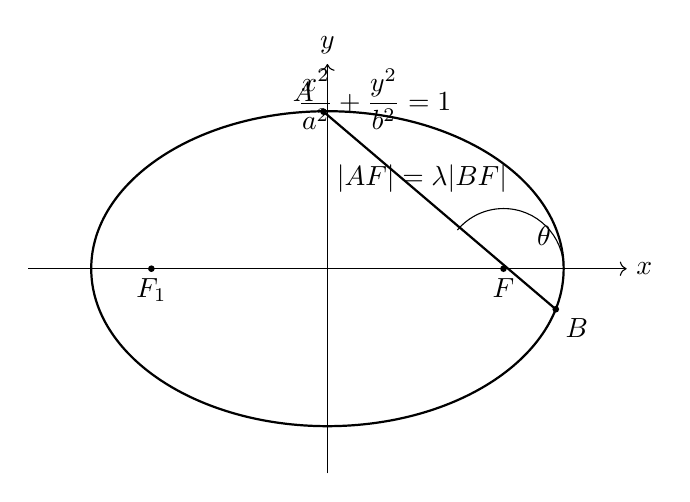
\begin{tikzpicture}[scale=1.0]
  \draw[->] (-3.8,0) -- (3.8,0) node[right] {$x$};
  \draw[->] (0,-2.6) -- (0,2.6) node[above] {$y$};
  \draw[thick] (0,0) ellipse (3 and 2);
  \fill (-2.236,0) circle (1.2pt) node[below] {$F_1$};
  \fill (2.236,0) circle (1.2pt) node[below] {$F$};
  \coordinate (A) at (-0.05,1.994);
  \coordinate (B) at (2.90,-0.515);
  \draw[thick] (A) -- (B);
  \fill (A) circle (1.2pt) node[above left] {$A$};
  \fill (B) circle (1.2pt) node[below right] {$B$};
  \draw[dashed] (2.236,0) -- ++(1.1,0);
  \draw (3.0,0) arc[start angle=0,end angle=140,radius=0.764];
  \node at (2.75,0.42) {$\theta$};
  \node at (1.2,1.15) {$|AF|=\lambda|BF|$};
  \node at (0.6,2.15) {$\dfrac{x^2}{a^2}+\dfrac{y^2}{b^2}=1$};
\end{tikzpicture}

\end{center}

\subsection*{对应高考真题}

\begin{gaokao}{2019 年高考数学 全国I卷-理科第10题}

已知椭圆 $C$ 的焦点为 $F_1(-1, 0)$, $F_2(1, 0)$，过 $F_2$ 的直线与 $C$ 交于 $A$, $B$ 两点．若 $|AF_2| = 2|F_2B|$, $|AB| = |BF_1|$, 则 $C$ 的方程为

\begin{enumerate}[label=\Alph*. ,itemsep=2pt]

\item $\frac{x^2}{2} + y^2 = 1$

\item $\frac{x^2}{3} + \frac{y^2}{2} = 1$

\item $\frac{x^2}{4} + \frac{y^2}{3} = 1$

\item $\frac{x^2}{5} + \frac{y^2}{4} = 1$

\end{enumerate}

\begin{center}

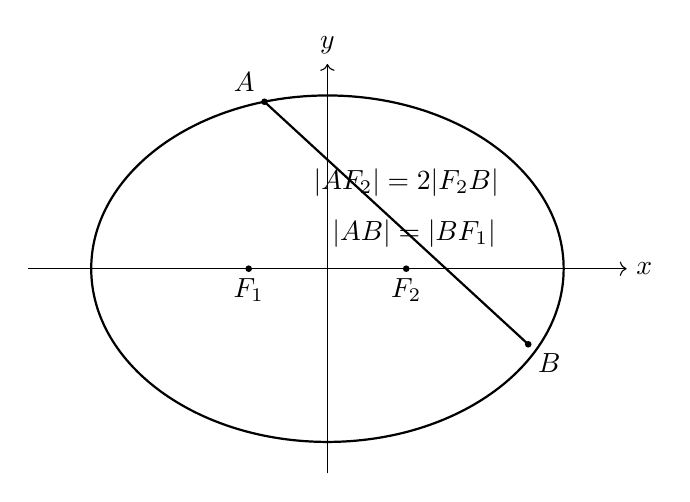
\begin{tikzpicture}[scale=1.0]
  \draw[->] (-3.8,0) -- (3.8,0) node[right] {$x$};
  \draw[->] (0,-2.6) -- (0,2.6) node[above] {$y$};
  \draw[thick] (0,0) ellipse (3 and 2.2);
  \fill (-1,0) circle (1.2pt) node[below] {$F_1$};
  \fill (1,0) circle (1.2pt) node[below] {$F_2$};
  \coordinate (A) at (-0.8,2.12);
  \coordinate (B) at (2.55,-0.96);
  \draw[thick] (A) -- (B);
  \fill (A) circle (1.2pt) node[above left] {$A$};
  \fill (B) circle (1.2pt) node[below right] {$B$};
  \node at (1.0,1.1) {$|AF_2|=2|F_2B|$};
  \node at (1.1,0.45) {$|AB|=|BF_1|$};
\end{tikzpicture}

\end{center}

\paragraph{技巧对应}

这题与本模型的对应最直接。题干中有“过 $F_2$ 的直线与椭圆交于 $A,B$ 两点”，这是典型的焦点弦背景；又已知 $|AF_2|=2|F_2B|$，可立即设 $\lambda=2$。虽然题目最终还给了 $|AB|=|BF_1|$ 这一附加条件，完整求解仍需结合椭圆定义与三角形性质，但“先把焦点分比读出来”正是本技巧的核心入口。也就是说，本题不是只考焦比弦公式本身，却非常适合作为“识别焦点弦分比信息”的真题样本。

\paragraph{答案}

$B$

\paragraph{解答}

如图，由已知可设 $|F_2B| = n$，则 $|AF_2| = 2n$, $|BF_1| = |AB| = 3n$，由椭圆的定义有 $2a = |BF_1| + |BF_2| = 4n$, $\therefore |AF_1| = 2a - |AF_2| = 2n$．在 $\triangle AF_1B$ 中，由余弦定理推论得 $\cos \angle F_1AB = \frac{4n^2 + 9n^2 - 9n^2}{2 \cdot 2n \cdot 3n} = \frac{1}{3}$．在 $\triangle AF_1F_2$ 中，由余弦定理得 $4n^2 + 4n^2 - 2 \cdot 2n \cdot 2n \cdot \frac{1}{3} = 4$，解得 $n = \frac{\sqrt{3}}{2}$．$\therefore 2a = 4n = 2\sqrt{3}$, $\therefore a = \sqrt{3}$, $\therefore b^2 = a^2 - c^2 = 3 - 1 = 2$, $\therefore$ 所求椭圆方程为 $\frac{x^2}{3} + \frac{y^2}{2} = 1$，故选 $B$．

\par\smallskip\textcolor{gray}{\footnotesize 来源记录：\texttt{\detokenize{tex版(exam-zh模板2016-2025)/2019/2019-全国I卷-理科/questions.json}}}

\end{gaokao}

\begin{gaokao}{2017 年高考数学 全国I卷-理科第10题}

已知 $F$ 为抛物线 $C:y^2=4x$ 的焦点，过 $F$ 作两条互相垂直的直线 $l_1$，$l_2$，直线 $l_1$ 与 $C$ 交于 $A$、$B$ 两点，直线 $l_2$ 与 $C$ 交于 $D$、$E$ 两点，则 $|AB|+|DE|$ 的最小值为（ ）

\begin{enumerate}[label=\Alph*. ,itemsep=2pt]

\item $16$

\item $14$

\item $12$

\item $10$

\end{enumerate}

\begin{center}

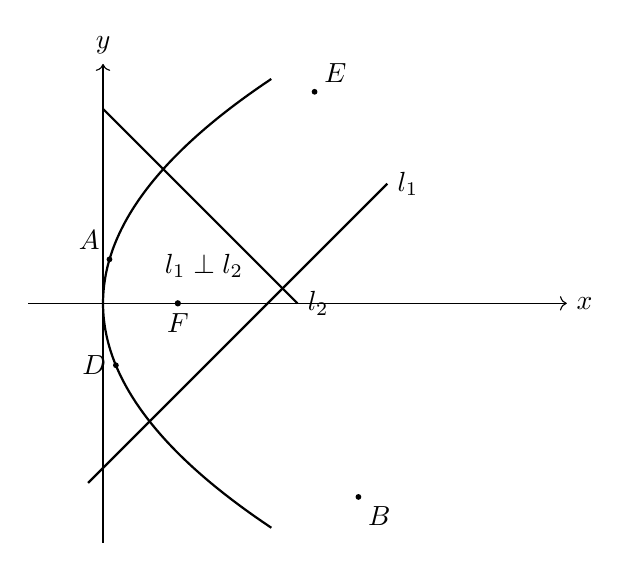
\begin{tikzpicture}[scale=0.95]
  \draw[->] (-1,0) -- (6.2,0) node[right] {$x$};
  \draw[->] (0,-3.2) -- (0,3.2) node[above] {$y$};
  \draw[thick,domain=-3:3,samples=120] plot ({\x*\x/4},{\x});
  \fill (1,0) circle (1.2pt) node[below] {$F$};
  \draw[thick] (-0.2,-2.4) -- (3.8,1.6) node[right] {$l_1$};
  \draw[thick] (0.0,2.6) -- (2.6,0.0) node[right] {$l_2$};
  \fill (0.086,0.588) circle (1.1pt) node[above left] {$A$};
  \fill (3.414,-2.588) circle (1.1pt) node[below right] {$B$};
  \fill (0.172,-0.828) circle (1.1pt) node[left] {$D$};
  \fill (2.828,2.828) circle (1.1pt) node[above right] {$E$};
  \node at (1.35,0.5) {$l_1\perp l_2$};
\end{tikzpicture}

\end{center}

\paragraph{技巧对应}

这题与抛物线焦点弦公式高度相关。题干中两条直线都过焦点，分别与抛物线交成两条焦点弦 $AB,DE$，并且两弦互相垂直。题解给出的“方法二”直接使用了抛物线过焦点弦长公式 $|AB|=\dfrac{2p}{\sin^2\theta}$，本质上就是焦点弦模型在长度问题中的标准落地。虽然它没有显式给出分比 $\lambda$，但它完整体现了本技巧所属的“过焦点弦，优先找角与弦长关系”的思路，因此与本条技巧有实质同源性。

\paragraph{答案}

A

\paragraph{解答}

方法一：如图，$l_1\perp l_2$，要使 $|AB|+|DE|$ 最小，则 $A$ 与 $D$，$B$，$E$ 关于 $x$ 轴对称，即直线 $DE$ 的斜率为 1，又直线 $l_2$ 过点 $(1,0)$，则直线 $l_2$ 的方程为 $y=x-1$，联立 $\begin{cases} y^2=4x \\ y=x-1 \end{cases}$，则 $y^2-4y-4=0$，\ensuremath{\therefore}$y_1+y_2=4$，$y_1y_2=-4$，\ensuremath{\therefore}$|DE|=\sqrt{1+1^2}\cdot|y_1-y_2|=\sqrt{2}\times\sqrt{4^2+16}=8$，\ensuremath{\therefore}$|AB|+|DE|$ 的最小值为 $2|DE|=16$．方法二：设直线 $l_1$ 的倾斜角为 $\theta$，则 $l_2$ 的倾斜角为 $\frac{\pi}{2}+\theta$，根据焦点弦长公式可得 $|AB|=\frac{2p}{\sin^2\theta}=\frac{4}{\sin^2\theta}$，$|DE|=\frac{4}{\sin^2(\frac{\pi}{2}+\theta)}=\frac{4}{\cos^2\theta}$，\ensuremath{\therefore}$|AB|+|DE|=\frac{4}{\sin^2\theta}+\frac{4}{\cos^2\theta}=\frac{4}{\sin^2\theta\cos^2\theta}=\frac{16}{\sin^2 2\theta}$，\ensuremath{\because}$0<\sin^2 2\theta\leq 1$，\ensuremath{\therefore}当 $\theta=45^\circ$ 时，$|AB|+|DE|$ 最小，最小为 16．故选：A．

\par\smallskip\textcolor{gray}{\footnotesize 来源记录：\texttt{\detokenize{tex版(exam-zh模板2016-2025)/2017/2017-全国I卷-理科/questions.json}}}

\end{gaokao}

\begin{gaokao}{2025 年高考数学 全国I卷第10题}

设抛物线 $C: y^2 = 6x$ 的焦点为 $F$，过 $F$ 的直线交 $C$ 于 $A$、$B$，过 $F$ 且垂直于 $AB$ 的直线交 $l: x = -\frac{3}{2}$ 于 $E$，过点 $A$ 作准线 $l$ 的垂线，垂足为 $D$，则（ ）

\begin{enumerate}[label=\Alph*. ,itemsep=2pt]

\item $|AD| = |AF|$

\item $|AE| = |AB|$

\item $|AB| \ge 6$

\item $|AE| \cdot |BE| \ge 18$

\end{enumerate}

\begin{center}

\begin{tikzpicture}[scale=0.95]
  \draw[->] (-2.2,0) -- (6.4,0) node[right] {$x$};
  \draw[->] (0,-4.0) -- (0,4.0) node[above] {$y$};
  \draw[thick,domain=-4.1:4.1,samples=160] plot ({\x*\x/6},{\x});
  \draw[dashed] (-1.5,-3.8) -- (-1.5,3.8) node[above] {$l:x=-\dfrac{3}{2}$};
  \fill (1.5,0) circle (1.2pt) node[below] {$F$};
  \coordinate (A) at (0.167,-1.0);
  \coordinate (B) at (5.167,5.0);
  \draw[thick] (A) -- (B);
  \fill (A) circle (1.1pt) node[below left] {$A$};
  \fill (B) circle (1.1pt) node[above right] {$B$};
  \draw[thick] (-0.7,1.833) -- (3.3,-1.5);
  \fill (-1.5,-1.5) circle (1.1pt) node[left] {$E$};
  \draw[dashed] (0.167,-1.0) -- (-1.5,-1.0);
  \fill (-1.5,-1.0) circle (1.1pt) node[left] {$D$};
  \node at (3.4,1.0) {$AB\perp FE$};
\end{tikzpicture}

\end{center}

\paragraph{技巧对应}

这题与技巧53的贴合度也很高。题干中“过 $F$ 的直线交 $C$ 于 $A,B$”直接给出抛物线焦点弦，后续又作过 $F$ 且垂直于 $AB$ 的直线，形成两条互相关联的焦点弦方向信息。官方解析中的 C、D 两项都用了过焦点弦的参数关系与长度关系，其中 C 项得到 $|AB|=6(m^2+1)\ge 6$，本质上仍是在利用焦点弦模型快速处理弦长。它比上一题更综合，但仍然保留了本技巧最关键的结构特征。

\paragraph{答案}

ACD

\paragraph{解答}

法一：对于 A，抛物线 $y^2=6x$，$p=3$，准线方程 $x=-\frac{3}{2}$，焦点 $F\left(\frac{3}{2},0\right)$，由抛物线定义，$|AD| = |AF|$，故 A 正确；对于 B，过点 $B$ 作准线垂线交于点 $P$，易证 $\triangle ADE \cong \triangle AFE$，$\triangle BEP \cong \triangle BEF$，则 $\angle AED = \angle AEF$，$\angle BEP = \angle BEF$，又 $\angle AED+\angle AEF+\angle BEP+\angle BEF=180^\circ$，所以 $\angle AEF+\angle BEF=90^\circ$，即 $\angle AEB=90^\circ$，$AB$ 为斜边，则 $|AE| < |AB|$，故 B 错误；对于 C，设直线 $AB$ 方程为 $x = my + \frac{3}{2}$，与 $y^2=6x$ 联立得 $y^2-6my-9=0$，$y_1+y_2=6m$，$y_1y_2=-9$，$|AB| = x_1+x_2+p = m(y_1+y_2)+3+3 = 6m^2+6 \ge 6$，当且仅当 $m=0$ 时取等号，故 C 正确；对于 D，在 $\triangle ABE$ 与 $\triangle AEF$ 中，$\angle BAE = \angle EAF$，所以 $\triangle ABE \sim \triangle AEF$，则 $\frac{AE}{AB} = \frac{AF}{AE}$，即 $AE^2 = AF \cdot AB$，同理 $BE^2 = BF \cdot AB$，$AF \cdot BF = (x_1+\frac{3}{2})(x_2+\frac{3}{2}) = (my_1+3)(my_2+3) = m^2 y_1 y_2 + 3m(y_1+y_2)+9 = -9m^2+18m^2+9 = 9(m^2+1)$，$AB = 6(m^2+1)$，则 $AE^2 \cdot BE^2 = BF \cdot AF \cdot AB^2 = 9(m^2+1) \times 36(m^2+1)^2$，所以 $AE \cdot BE = 3(m^2+1)^{\frac{1}{2}} \times 6(m^2+1) = 18(m^2+1)^{\frac{3}{2}} \ge 18$，故 D 正确. 故选：ACD. 法二：略.

\par\smallskip\textcolor{gray}{\footnotesize 来源记录：\texttt{\detokenize{tex版(exam-zh模板2016-2025)/2025/2025-全国I卷/questions.json}}}

\end{gaokao}

\clearpage

\section{技巧54：圆锥曲线切线问题}

\subsection*{核心认识}

圆锥曲线切线问题常见为两类：一类是\underline{过曲线上一点}求切线，另一类是\underline{过曲线外一点}作两条切线并研究两切点连线。处理这类题时，关键不是每次都从判别式重推，而是优先识别是否可以直接调用标准结论。

对椭圆、双曲线、抛物线，若已知切点 $P(x_0,y_0)$ 在曲线上，则切线方程通常可由对应的“点式切线公式”直接写出；若已知曲线外一点 $P(x_0,y_0)$ 向曲线引两条切线，切点分别为 $A,B$，则直线 $AB$ 往往可由“切点弦方程”直接写出。例如：
\[
\text{椭圆 }\frac{x^2}{a^2}+\frac{y^2}{b^2}=1\Rightarrow \frac{x_0x}{a^2}+\frac{y_0y}{b^2}=1,
\]
\[
\text{双曲线 }\frac{x^2}{a^2}-\frac{y^2}{b^2}=1\Rightarrow \frac{x_0x}{a^2}-\frac{y_0y}{b^2}=1,
\]
\[
\text{抛物线 }y^2=2px\Rightarrow y_0y=p(x+x_0).
\]

要注意：直线与圆锥曲线只有一个公共点，并不一定就是切线。双曲线中平行于渐近线的某些直线、抛物线中平行于对称轴的某些直线，都可能只与曲线有一个公共点，但并不是切线。

\subsection*{操作步骤}

\begin{enumerate}

\item 先判断题型：是“过曲线上一点求切线”，还是“过曲线外一点作两条切线并研究切点弦”。

\item 若已知切点坐标，直接写点式切线方程；不要先设斜率、再联立、再令判别式为零。

\item 若已知曲线外一点 $P(x_0,y_0)$，且从该点向圆锥曲线引两条切线，切点为 $A,B$，则优先写出切点弦 $AB$ 的方程。

\item 遇到“定点、定斜率、平行、垂直、中点、面积”这类结论时，先把切线或切点弦方程化成直线一般式，再读出斜率或代入特殊点验证。

\item 若题目中的直线只是与曲线“有唯一公共点”，必须再核查它是否真是切线，不能把“唯一交点”等同于“相切”。

\end{enumerate}

\subsection*{结构图}

\begin{center}

\begin{tikzpicture}[scale=0.9]
  \draw[->] (-4.2,0) -- (4.8,0) node[right] {$x$};
  \draw[->] (0,-3.2) -- (0,3.6) node[above] {$y$};
  \draw[thick] (0,0) ellipse [x radius=3, y radius=2];
  \coordinate (P) at (4.1,1.2);
  \coordinate (A) at (1.44,1.75);
  \coordinate (B) at (2.56,-1.04);
  \draw[thick] (P)--(A);
  \draw[thick] (P)--(B);
  \draw[dashed] (A)--(B);
  \fill (P) circle (1.5pt) node[right] {$P(x_0,y_0)$};
  \fill (A) circle (1.5pt) node[above] {$A$};
  \fill (B) circle (1.5pt) node[below] {$B$};
  \node at (0,-2.55) {$\displaystyle \frac{x^2}{a^2}+\frac{y^2}{b^2}=1$};
  \node at (1.6,2.6) {$PA,PB$ 为切线};
  \node at (2.35,0.7) {$AB$ 为切点弦};
\end{tikzpicture}

\end{center}

\subsection*{对应高考真题}

\begin{gaokao}{2019 年高考数学 全国III卷-理科第21题}

已知曲线 $C: y=\dfrac{x^2}{2}$，$D$ 为直线 $y=-\dfrac{1}{2}$ 上的动点，过 $D$ 作 $C$ 的两条切线，切点分别为 $A$，$B$。
（1）证明：直线 $AB$ 过定点；
（2）若以 $E\left(0,\dfrac{5}{2}\right)$ 为圆心的圆与直线 $AB$ 相切，且切点为线段 $AB$ 的中点，求四边形 $ADBE$ 的面积。

\begin{center}

\begin{tikzpicture}[scale=0.95]
  \draw[->] (-2.2,0) -- (4.4,0) node[right] {$x$};
  \draw[->] (0,-1.4) -- (0,4.4) node[above] {$y$};
  \draw[thick,domain=0:2.8,samples=120] plot(\x,{0.5*\x*\x});
  \draw[dashed] (-2.0,-0.5)--(4.2,-0.5) node[right] {$y=-\frac12$};
  \coordinate (D) at (2.2,-0.5);
  \coordinate (A) at (1,0.5);
  \coordinate (B) at (-0.4142,0.0858);
  \draw[thick] (D)--(A);
  \draw[thick] (D)--(B);
  \draw[dashed] (A)--(B);
  \fill (D) circle (1.4pt) node[below right] {$D$};
  \fill (A) circle (1.4pt) node[above right] {$A$};
  \fill (B) circle (1.4pt) node[above left] {$B$};
  \node at (2.9,3.7) {$C:y=\dfrac{x^2}{2}$};
  \node at (1.2,1.35) {$AB$};
\end{tikzpicture}

\end{center}

\paragraph{技巧对应}

这道题与本技巧的对应最直接。题设是“过直线上的动点 $D$ 作抛物线 $C:y=\dfrac{x^2}{2}$ 的两条切线，切点分别为 $A,B$”，本质上正是“过曲线外一点作抛物线的两条切线”。题解第（1）问得到 $AB$ 的方程为 $2tx-2y+1=0$，这与抛物线 $y^2=2x$ 的切点弦公式 $y_0y=x+x_0$ 完全一致：当 $D(t,-\tfrac12)$ 时，代入可得 $-\tfrac12 y=x+t$，即 $2tx-2y+1=0$ 的同类结构。该题充分体现了：一旦识别出“外点引两切线”，就应优先考虑切点弦方程，从而快速得到定点、面积等结论。

\paragraph{答案}

（1）定点为 $\left(0,\dfrac{1}{2}\right)$；（2）四边形 $ADBE$ 的面积为 $3$ 或 $4\sqrt{2}$。

\paragraph{解答}

（1）设 $D\left(t,-\dfrac{1}{2}\right)$，$A(x_1,y_1)$，则 $x_1^2=2y_1$。由于 $y'=x$，所以切线 $DA$ 的斜率为 $x_1$，故 $\dfrac{y_1+\frac{1}{2}}{x_1-t}=x_1$，整理得 $2tx_1-2y_1+1=0$。设 $B(x_2,y_2)$，同理可得 $2tx_2-2y_2+1=0$。故直线 $AB$ 的方程为 $2tx-2y+1=0$，所以直线 $AB$ 过定点 $\left(0,\dfrac{1}{2}\right)$。
（2）由（1）得直线 $AB$ 的方程为 $y=tx+\dfrac{1}{2}$。与 $y=\dfrac{x^2}{2}$ 联立得 $x^2-2tx-1=0$，于是 $x_1+x_2=2t$，$x_1x_2=-1$，$y_1+y_2=t(x_1+x_2)+1=2t^2+1$，$|AB|=\sqrt{1+t^2}|x_1-x_2|=\sqrt{1+t^2}\times\sqrt{(x_1+x_2)^2-4x_1x_2}=2(t^2+1)$。设 $d_1,d_2$ 分别为点 $D$，$E$ 到直线 $AB$ 的距离，则 $d_1=\sqrt{t^2+1}$，$d_2=\dfrac{2}{\sqrt{t^2+1}}$。因此四边形 $ADBE$ 的面积 $S=\dfrac{1}{2}|AB|(d_1+d_2)=(t^2+3)\sqrt{t^2+1}$。设 $M$ 为线段 $AB$ 的中点，则 $M\left(t,t^2+\dfrac{1}{2}\right)$。由于 $\overrightarrow{EM}\perp\overrightarrow{AB}$，而 $\overrightarrow{EM}=(t,t^2-2)$，$\overrightarrow{AB}$ 与向量 $(1,t)$ 平行，所以 $t+(t^2-2)t=0$，解得 $t=0$ 或 $t=\pm1$。当 $t=0$ 时，$S=3$；当 $t=\pm1$ 时，$S=4\sqrt{2}$。因此，四边形 $ADBE$ 的面积为 $3$ 或 $4\sqrt{2}$。

\par\smallskip\textcolor{gray}{\footnotesize 来源记录：\texttt{\detokenize{tex版(exam-zh模板2016-2025)/2019/2019-全国III卷-理科/questions.json}}}

\end{gaokao}

\begin{gaokao}{2021 年高考数学 全国乙卷-理科第21题}

已知抛物线$C:x^2=2py$（$p>0$）的焦点为$F$，且$F$与圆$M:x^2+(y+4)^2=1$上点的距离的最小值为4。
（1）求$p$；
（2）若点$P$在$M$上，$PA$，$PB$是$C$的两条切线，$A$，$B$是切点，求$\triangle PAB$面积的最大值。

\begin{center}

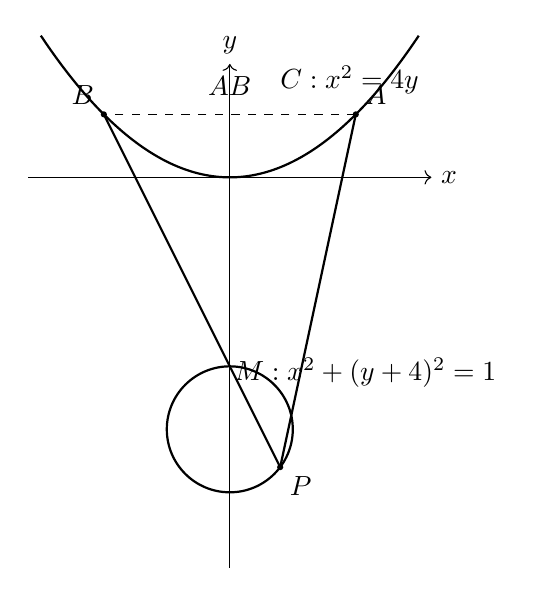
\begin{tikzpicture}[scale=0.8]
  \draw[->] (-3.2,0) -- (3.2,0) node[right] {$x$};
  \draw[->] (0,-6.2) -- (0,1.8) node[above] {$y$};
  \draw[thick,domain=-3:3,samples=120] plot(\x,{0.25*\x*\x});
  \draw[thick] (0,-4) circle (1);
  \coordinate (P) at (0.8,-4.6);
  \coordinate (A) at (2,1);
  \coordinate (B) at (-2,1);
  \draw[thick] (P)--(A);
  \draw[thick] (P)--(B);
  \draw[dashed] (A)--(B);
  \fill (P) circle (1.4pt) node[below right] {$P$};
  \fill (A) circle (1.4pt) node[above right] {$A$};
  \fill (B) circle (1.4pt) node[above left] {$B$};
  \node at (2.15,-3.1) {$M:x^2+(y+4)^2=1$};
  \node at (1.9,1.55) {$C:x^2=4y$};
  \node at (0,1.45) {$AB$};
\end{tikzpicture}

\end{center}

\paragraph{技巧对应}

这道题同样属于“过曲线外一点作抛物线的两条切线”，而且第（2）问直接把技巧用到了面积最值中。题解先由切点 $A(x_1,y_1)$、$B(x_2,y_2)$ 写出切线，再由点 $P(x_0,y_0)$ 同时在两条切线上，推出 $AB$ 的方程为 $y=\dfrac12 x_0x-y_0$。这正是抛物线 $x^2=2py$ 在外点 $P(x_0,y_0)$ 的切点弦公式 $x_0x=p(y+y_0)$ 在本题 $p=2$ 情形下的等价形式。题目说明：切点弦公式不仅能解决定点、定值问题，还能显著简化面积与最值计算。

\paragraph{答案}

（1）$p=2$；（2）$20\sqrt{5}$

\paragraph{解答}

（1）焦点$F(0,\frac{p}{2})$到圆$x^2+(y+4)^2=1$的最短距离为$\frac{p}{2}+3=4$，所以$p=2$。
（2）抛物线$y=\frac14x^2$，设$A(x_1,y_1)$，$B(x_2,y_2)$，$P(x_0,y_0)$，得$l_{PA}: y=\frac12x_1(x-x_1)+y_1=\frac12x_1x-\frac14x_1^2=\frac12x_1x-y_1$，$l_{PB}: y=\frac12x_2x-y_2$，且$x_0^2=-y_0^2-8y_0-15$。$l_{PA}$，$l_{PB}$都过点$P(x_0,y_0)$，则$\begin{cases} y_0=\frac12x_1x_0-y_1 \\ y_0=\frac12x_2x_0-y_2 \end{cases}$，故$l_{AB}: y_0=\frac12x_0x-y$，即$y=\frac12x_0x-y_0$。联立$\begin{cases} y=\frac12x_0x-y_0 \\ x^2=4y \end{cases}$，得$x^2-2x_0x+4y_0=0$，$\Delta=4x_0^2-16y_0$。所以$|AB|=\sqrt{1+\frac{x_0^2}{4}}\cdot\sqrt{4x_0^2-16y_0}=\sqrt{4+x_0^2}\cdot\sqrt{x_0^2-4y_0}$，$d_{P\to AB}=\frac{|x_0^2-4y_0|}{\sqrt{x_0^2+4}}$，所以$S_{\triangle PAB}=\frac12|AB|\cdot d_{P\to AB}=\frac12\sqrt{x_0^2-4y_0}\cdot\sqrt{x_0^2-4y_0}=\frac12(x_0^2-4y_0)^{\frac32}=\frac12(-y_0^2-12y_0-15)^{\frac32}$。而$y_0\in[-5,-3]$，故当$y_0=-5$时，$S_{\triangle PAB}$达到最大，最大值为$20\sqrt{5}$。

\par\smallskip\textcolor{gray}{\footnotesize 来源记录：\texttt{\detokenize{tex版(exam-zh模板2016-2025)/2021/2021-全国乙卷-理科/questions.json}}}

\end{gaokao}

\begin{gaokao}{2021 年高考数学 天津卷第18题}

已知椭圆 $\frac{x^2}{a^2} + \frac{y^2}{b^2} = 1$ ($a > b > 0$) 的右焦点为 $F$，上顶点为 $B$，离心率为 $\frac{2\sqrt{5}}{5}$，且 $|BF| = \sqrt{5}$．
（I）求椭圆的方程；
（II）直线 $l$ 与椭圆有唯一的公共点 $M$，与 $y$ 轴的正半轴交于点 $N$，过 $N$ 与 $BF$ 垂直的直线交 $x$ 轴于点 $P$．若 $MP // BF$，求直线 $l$ 的方程．

\begin{center}

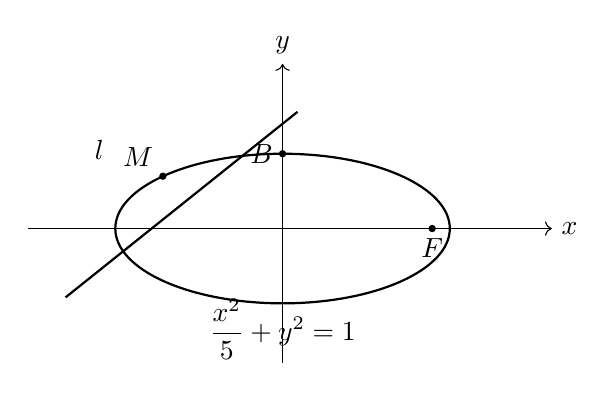
\begin{tikzpicture}[scale=0.95]
  \draw[->] (-3.4,0) -- (3.6,0) node[right] {$x$};
  \draw[->] (0,-1.8) -- (0,2.2) node[above] {$y$};
  \draw[thick] (0,0) ellipse [x radius=2.236, y radius=1];
  \coordinate (F) at (2,0);
  \coordinate (B) at (0,1);
  \coordinate (M) at (-1.6,0.6997);
  \draw[thick] (-2.9,-0.92)--(0.2,1.56);
  \draw[dashed] (0,0)--(F);
  \draw[dashed] (0,0)--(B);
  \fill (F) circle (1.4pt) node[below] {$F$};
  \fill (B) circle (1.4pt) node[left] {$B$};
  \fill (M) circle (1.4pt) node[above left] {$M$};
  \node at (0,-1.35) {$\displaystyle \frac{x^2}{5}+y^2=1$};
  \node at (-2.45,1.05) {$l$};
\end{tikzpicture}

\end{center}

\paragraph{技巧对应}

这道题对应的是“过曲线上一点作椭圆的切线”。第（II）问设椭圆上一点 $M(x_0,y_0)$ 后，直接写出切线方程 $\dfrac{x_0x}{5}+y_0y=1$，这是椭圆点式切线公式的标准应用。它非常适合作为本技巧中“已知切点，直接写切线”的典型真题。与前两题相比，本题不涉及外点引两切线，而是突出另一类核心场景：已知切点时，利用点式切线公式进行后续几何关系推导。

\paragraph{答案}

（I）$\frac{x^2}{5} + y^2 = 1$；（II）$x - y + \sqrt{6} = 0$

\paragraph{解答}

（I）$F(c,0)$，$B(0,b)$，$|BF| = \sqrt{c^2+b^2} = a = \sqrt{5}$，离心率 $e = \frac{c}{a} = \frac{2\sqrt{5}}{5}$，得 $c=2$，$b = \sqrt{a^2-c^2} = 1$，所以椭圆方程为 $\frac{x^2}{5} + y^2 = 1$；
（II）设 $M(x_0,y_0)$ 为椭圆上一点，则椭圆在 $M$ 处的切线方程为 $\frac{x_0 x}{5} + y_0 y = 1$，令 $x=0$ 得 $N\left(0,\frac{1}{y_0}\right)$，$BF$ 斜率为 $k_{BF} = -\frac{b}{c} = -\frac{1}{2}$，则 $PN$ 方程为 $y = 2x + \frac{1}{y_0}$，令 $y=0$ 得 $P\left(-\frac{1}{2y_0},0\right)$，$k_{MP} = \frac{y_0}{x_0+\frac{1}{2y_0}} = \frac{2y_0^2}{2x_0 y_0+1}$，由 $MP // BF$ 得 $\frac{2y_0^2}{2x_0 y_0+1} = -\frac{1}{2}$，整理得 $(x_0+5y_0)^2=0$，所以 $x_0 = -5y_0$，代入椭圆方程得 $\frac{25y_0^2}{5}+y_0^2=6y_0^2=1$，$y_0 = \frac{\sqrt{6}}{6}$，$x_0 = -\frac{5\sqrt{6}}{6}$，所以直线 $l$ 方程为 $\frac{-\frac{5\sqrt{6}}{6}x}{5} + \frac{\sqrt{6}}{6}y = 1$，即 $x - y + \sqrt{6}=0$.

\par\smallskip\textcolor{gray}{\footnotesize 来源记录：\texttt{\detokenize{tex版(exam-zh模板2016-2025)/2021/2021-天津卷/questions.json}}}

\end{gaokao}

\clearpage

\section{技巧55：双曲线离心率与渐近线倾斜角的关系}

\subsection*{核心认识}

对双曲线 $\dfrac{x^2}{a^2}-\dfrac{y^2}{b^2}=1\,(a>0,b>0)$，其渐近线为 $y=\pm \dfrac{b}{a}x$。若其中一条渐近线的倾斜角为 $\theta$，且取 $\theta\in\left(0,\dfrac{\pi}{2}\right)$ 对应正斜率渐近线，则
\[
\tan\theta=\frac{b}{a},\qquad e=\frac{c}{a}=\sqrt{1+\frac{b^2}{a^2}}=\sqrt{1+\tan^2\theta}=\frac{1}{\cos\theta}.
\]
因此，已知双曲线为横轴型且已知某条渐近线的倾斜角，就可以直接由 $e=\dfrac{1}{\cos\theta}$ 求离心率。反过来，若已知离心率 $e$，则有
\[
\frac{b}{a}=\sqrt{e^2-1},
\]
从而可写出渐近线方程 $y=\pm \sqrt{e^2-1}\,x$。若题目给出的倾斜角大于 $90^\circ$，应先利用另一条渐近线或结合三角函数把斜率化为正斜率形式再代入。

\subsection*{操作步骤}

\begin{enumerate}

\item 先判断双曲线类型：若是 $\dfrac{x^2}{a^2}-\dfrac{y^2}{b^2}=1$，则使用 $y=\pm \dfrac{b}{a}x$；若是 $\dfrac{y^2}{a^2}-\dfrac{x^2}{b^2}=1$，则使用 $y=\pm \dfrac{a}{b}x$。

\item 把“渐近线倾斜角”转化为“渐近线斜率”：横轴型中有 $\tan\theta=\dfrac{b}{a}$；若已给的是钝角倾斜角，要先由图形或三角函数关系化到锐角。

\item 遇到横轴型双曲线且已知锐角倾斜角 $\theta$ 时，直接套用
\[
e=\sqrt{1+\tan^2\theta}=\frac{1}{\cos\theta}.
\]

\item 若已知离心率 $e$，则先求
\[
\frac{b}{a}=\sqrt{e^2-1},
\]
再写渐近线方程 $y=\pm \dfrac{b}{a}x$。

\item 若题目外层包裹了焦点、圆、距离、垂直等条件，最后仍需回到“求出渐近线斜率”这一步，再转化为离心率。

\end{enumerate}

\subsection*{结构图}

\begin{center}

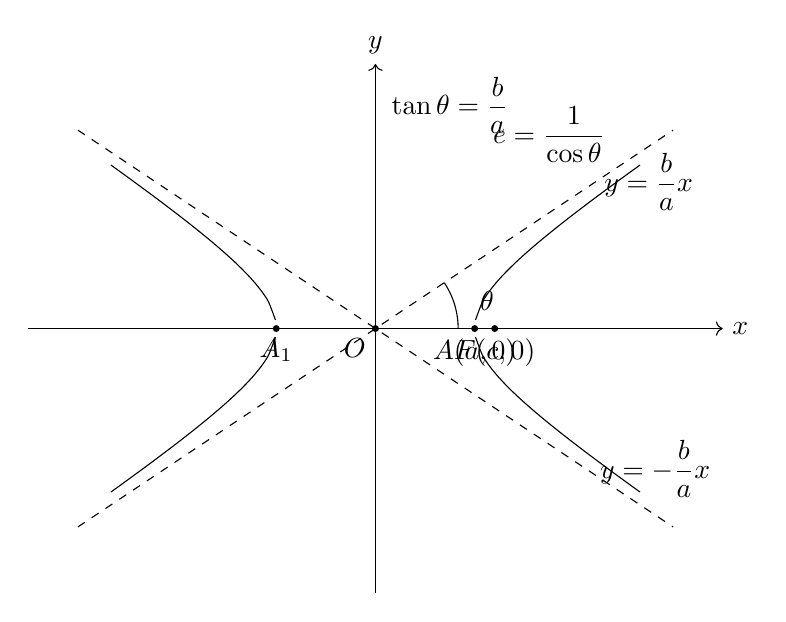
\begin{tikzpicture}[scale=1.05]
  \draw[->] (-4.2,0)--(4.2,0) node[right]{$x$};
  \draw[->] (0,-3.2)--(0,3.2) node[above]{$y$};
  \draw[dashed] (-3.6,-2.4)--(3.6,2.4);
  \draw[dashed] (-3.6,2.4)--(3.6,-2.4);
  \draw[domain=-3.2:-1.21,smooth,variable=\x] plot ({\x},{sqrt((\x*\x/1.44-1)*0.64)});
  \draw[domain=-3.2:-1.21,smooth,variable=\x] plot ({\x},{-sqrt((\x*\x/1.44-1)*0.64)});
  \draw[domain=1.21:3.2,smooth,variable=\x] plot ({\x},{sqrt((\x*\x/1.44-1)*0.64)});
  \draw[domain=1.21:3.2,smooth,variable=\x] plot ({\x},{-sqrt((\x*\x/1.44-1)*0.64)});
  \fill (0,0) circle(1.2pt) node[below left]{$O$};
  \fill (1.2,0) circle(1.2pt) node[below]{$A(a,0)$};
  \fill (-1.2,0) circle(1.2pt) node[below]{$A_1$};
  \fill (1.442,0) circle(1.2pt) node[below]{$F(c,0)$};
  \draw (1.0,0) arc[start angle=0,end angle=33.69,radius=1.0];
  \node at (1.35,0.33){$\theta$};
  \node[right] at (2.65,1.77){$y=\dfrac{b}{a}x$};
  \node[right] at (2.6,-1.7){$y=-\dfrac{b}{a}x$};
  \node at (0.9,2.7){$\tan\theta=\dfrac{b}{a}$};
  \node at (2.1,2.35){$e=\dfrac{1}{\cos\theta}$};
\end{tikzpicture}

\end{center}

\subsection*{对应高考真题}

\begin{gaokao}{2019 年高考数学 全国I卷-文科第10题}

双曲线 $C: \frac{x^2}{a^2} - \frac{y^2}{b^2} = 1$ ($a>0,b>0$) 的一条渐近线的倾斜角为 130°，则 $C$ 的离心率为

\begin{enumerate}[label=\Alph*. ,itemsep=2pt]

\item $2\sin40°$

\item $2\cos40°$

\item $\frac{1}{\sin50°}$

\item $\frac{1}{\cos50°}$

\end{enumerate}

\paragraph{技巧对应}

这道题与本技巧完全同构。题干直接给出横轴型双曲线的一条渐近线倾斜角为 $130^\circ$，核心就是把倾斜角转化为渐近线斜率，再由
\[
e=\sqrt{1+\left(\frac{b}{a}\right)^2}=\frac{1}{\cos 50^\circ}
\]
求离心率。它最能体现“由渐近线倾斜角直接求离心率”的模型，只是题目给的是钝角，需要先化为与正斜率对应的锐角 $50^\circ$，这也正好能训练学生对倾斜角概念的辨析。

\paragraph{答案}

D

\paragraph{解答}

由已知可得 $-\frac{b}{a} = \tan130°$，$\Rightarrow \frac{b}{a} = \tan50°$，$\Rightarrow e = \frac{c}{a} = \sqrt{1+\left(\frac{b}{a}\right)^2} = \sqrt{1+\tan^2 50°} = \sqrt{1+\frac{\sin^2 50°}{\cos^2 50°}} = \sqrt{\frac{\sin^2 50°+\cos^2 50°}{\cos^2 50°}} = \frac{1}{\cos50°}$，故选 D。

\par\smallskip\textcolor{gray}{\footnotesize 来源记录：\texttt{\detokenize{tex版(exam-zh模板2016-2025)/2019/2019-全国I卷-文科/questions.json}}}

\end{gaokao}

\begin{gaokao}{2020 年高考数学 全国III卷-文科第14题}

设双曲线 $C:\frac{x^2}{a^2}-\frac{y^2}{b^2}=1\ (a>0,b>0)$ 的一条渐近线为 $y=\sqrt{2}x$，则 $C$ 的离心率为

\paragraph{技巧对应}

这道题是本技巧的最直接基础型。题目直接给出一条渐近线为 $y=\sqrt{2}x$，立刻得到 $\dfrac{b}{a}=\sqrt{2}$，从而
\[
e=\sqrt{1+\frac{b^2}{a^2}}=\sqrt{3}.
\]
它没有额外几何包装，能最清楚地呈现“渐近线斜率 $\to$ 离心率”的主线，适合放在技巧讲解中的首题或例题。

\paragraph{答案}

$\sqrt{3}$

\paragraph{解答}

由双曲线方程可得其焦点在 $x$ 轴上，因为其一条渐近线为 $y=\sqrt{2}x$，所以 $\frac{b}{a}=\sqrt{2}$，$e=\frac{c}{a}=\sqrt{1+\frac{b^2}{a^2}}=\sqrt{3}$.

\par\smallskip\textcolor{gray}{\footnotesize 来源记录：\texttt{\detokenize{tex版(exam-zh模板2016-2025)/2020/2020-全国III卷-文科/questions.json}}}

\end{gaokao}

\begin{gaokao}{2021 年高考数学 新高考II卷第13题}

已知双曲线$\frac{x^2}{a^2}-\frac{y^2}{b^2}=1(a>0,b>0)$的离心率为$2$，则该双曲线的渐近线方程为\underline{\hspace{3cm}}

\paragraph{技巧对应}

这道题与前两题形成良好的双向对应。前两题是“由渐近线求离心率”，本题则是“由离心率求渐近线”。由 $e=2$ 得
\[
\frac{b}{a}=\sqrt{e^2-1}=\sqrt{3},
\]
于是渐近线方程为 $y=\pm\sqrt{3}x$。它能帮助学生把本技巧理解为双向转化关系，而不只是一条单向公式。

\paragraph{答案}

$y=\pm\sqrt{3}x$

\paragraph{解答}

因为双曲线$\frac{x^2}{a^2}-\frac{y^2}{b^2}=1(a>0,b>0)$的离心率为$2$，所以$e^2=\frac{c^2}{a^2}=\frac{a^2+b^2}{a^2}=2$，所以$\frac{b^2}{a^2}=3$，所以该双曲线的渐近线方程为$y=\pm\frac{b}{a}x=\pm\sqrt{3}x$.故答案为：$y=\pm\sqrt{3}x$.

\par\smallskip\textcolor{gray}{\footnotesize 来源记录：\texttt{\detokenize{tex版(exam-zh模板2016-2025)/2021/2021-新高考II卷/questions.json}}}

\end{gaokao}

\clearpage

\section{技巧56：超级韦达定理}

\subsection*{核心认识}

所谓“超级韦达定理”，本质上是把“定点与圆锥曲线上的两交点”这一几何关系，转化为关于过该定点的两条连线斜率的一元二次方程，再用韦达定理处理斜率和、斜率积或垂直关系。常见背景是：一条不过定点 $P(x_0,y_0)$ 的直线与椭圆、双曲线或抛物线交于两点 $A,B$，然后研究 $PA,PB$ 的斜率 $k_1,k_2$。操作时，先把曲线方程改写成关于 $x-x_0,y-y_0$ 的形式，再利用所给直线方程把常数项替换掉，最后除以 $(x-x_0)^2$，得到以 $k=\dfrac{y-y_0}{x-x_0}$ 为未知数的二次方程，其两根正是 $k_1,k_2$。这样可直接由韦达定理得到 $k_1+k_2,k_1k_2$，从而处理“斜率和为定值”“两线垂直”“点积恒正或恒负”“过定点”等问题。使用前提是：所设直线不能经过定点 $P$，并且所研究的两条连线斜率都存在。

\subsection*{操作步骤}

\begin{enumerate}

\item 设圆锥曲线为 $C$，定点为 $P(x_0,y_0)$，不过点 $P$ 的动直线设为 $l: p(x-x_0)+q(y-y_0)=1\,(p,q\text{不同时为}0)$。

\item 把圆锥曲线方程改写成含 $(x-x_0)$、$(y-y_0)$ 的形式。例如椭圆可写成 $\dfrac{[(x-x_0)+x_0]^2}{m}+\dfrac{[(y-y_0)+y_0]^2}{n}=1$。

\item 利用直线方程中的 $1=p(x-x_0)+q(y-y_0)$，常配合平方，代入曲线方程，把原式化为关于 $(x-x_0),(y-y_0)$ 的二次齐次关系。

\item 两边同除以 $(x-x_0)^2$，并令 $k=\dfrac{y-y_0}{x-x_0}$，得到一个关于 $k$ 的一元二次方程。

\item 该方程的两个实根就是 $k_{PA},k_{PB}$，再由韦达定理求出 $k_{PA}+k_{PB}$ 与 $k_{PA}k_{PB}$。

\item 若题目给出 $PA\perp PB$，则可直接用 $k_{PA}k_{PB}=-1$；若给出向量点积条件，如 $\overrightarrow{PA}\cdot\overrightarrow{PB}\le 0$，也常可先转化为关于 $k_{PA}+k_{PB},k_{PA}k_{PB}$ 的代数条件。

\item 最后把所得参数关系还原到动直线方程中，进而求定点、参数范围或证明结论。

\end{enumerate}

\subsection*{结构图}

\begin{center}

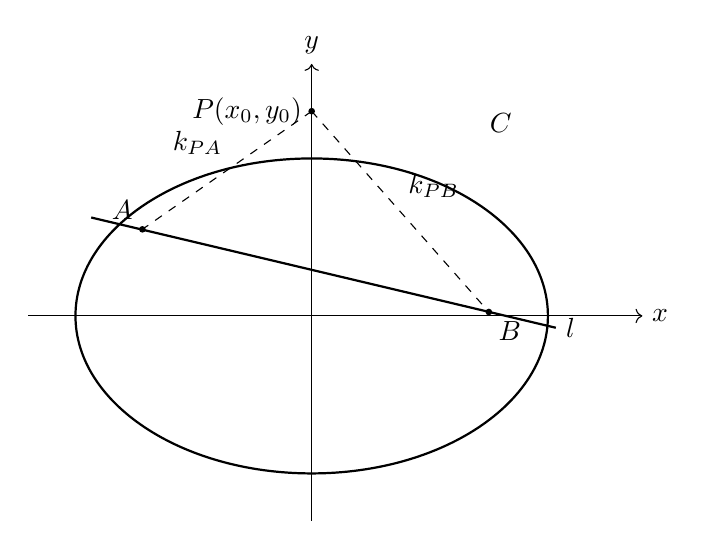
\begin{tikzpicture}[scale=1.0]
  \draw[->] (-3.6,0) -- (4.2,0) node[right] {$x$};
  \draw[->] (0,-2.6) -- (0,3.2) node[above] {$y$};
  \draw[thick] (0,0) ellipse (3 and 2);
  \fill (0,2.6) circle (1.2pt) node[left] {$P(x_0,y_0)$};
  \coordinate (A) at (-2.15,1.1);
  \coordinate (B) at (2.25,0.05);
  \draw[thick] (-2.8,1.25) -- (3.1,-0.15) node[right] {$l$};
  \fill (A) circle (1.2pt) node[above left] {$A$};
  \fill (B) circle (1.2pt) node[below right] {$B$};
  \draw[dashed] (0,2.6) -- (A);
  \draw[dashed] (0,2.6) -- (B);
  \node at (-1.45,2.2) {$k_{PA}$};
  \node at (1.55,1.65) {$k_{PB}$};
  \node at (2.4,2.45) {$C$};
\end{tikzpicture}

\end{center}

\subsection*{对应高考真题}

\begin{gaokao}{2017 年高考数学 全国I卷-理科第20题}

已知椭圆 $C:\frac{x^2}{a^2}+\frac{y^2}{b^2}=1$（$a>b>0$），四点 $P_1(1,1)$，$P_2(0,1)$，$P_3(-1,\frac{\sqrt{3}}{2})$，$P_4(1,\frac{\sqrt{3}}{2})$ 中恰有三点在椭圆 $C$ 上．
（1）求 $C$ 的方程；
（2）设直线 $l$ 不经过 $P_2$ 点且与 $C$ 相交于 $A$，$B$ 两点．若直线 $P_2A$ 与直线 $P_2B$ 的斜率的和为 $-1$，证明：$l$ 过定点．

\paragraph{技巧对应}

这道题与该方法的对应度最高。题设固定点为 $P_2(0,1)$，动直线 $l$ 不过 $P_2$，与椭圆交于 $A,B$，并直接给出 $P_2A,P_2B$ 的斜率和为 $-1$。这正是“把交点信息转化为过定点两连线的斜率关系”的标准场景。若按超级韦达定理设 $l:px+q(y-1)=1$，联立椭圆 $\dfrac{x^2}{4}+y^2=1$ 后可直接构造出关于 $k=\dfrac{y-1}{x}$ 的二次方程，其两根就是 $k_{P_2A},k_{P_2B}$，再由 $k_{P_2A}+k_{P_2B}=-1$ 反推出 $p,q$ 的关系，最终得到直线 $l$ 过定点。题目考查目标、设点方式、斜率条件和结论类型都与该技巧完全同构。

\paragraph{答案}

（1）$\frac{x^2}{4}+y^2=1$；（2）证明见解析，定点为 $(2,-1)$

\paragraph{解答}

解：（1）根据椭圆的对称性，$P_3(-1,\frac{\sqrt{3}}{2})$，$P_4(1,\frac{\sqrt{3}}{2})$ 两点必在椭圆 $C$ 上，又 $P_4$ 的横坐标为 1，\ensuremath{\therefore}椭圆必不过 $P_1(1,1)$，\ensuremath{\therefore}$P_2(0,1)$，$P_3(-1,\frac{\sqrt{3}}{2})$，$P_4(1,\frac{\sqrt{3}}{2})$ 三点在椭圆 $C$ 上．把 $P_2(0,1)$，$P_3(-1,\frac{\sqrt{3}}{2})$ 代入椭圆 $C$，得：$\begin{cases} \frac{0}{a^2}+\frac{1}{b^2}=1 \\ \frac{1}{a^2}+\frac{3}{4b^2}=1 \end{cases}$，解得 $a^2=4$，$b^2=1$，\ensuremath{\therefore}椭圆 $C$ 的方程为 $\frac{x^2}{4}+y^2=1$．
证明：（2）(1)当斜率不存在时，设 $l:x=m$，$A(m,y_A)$，$B(m,-y_A)$，\ensuremath{\because}直线 $P_2A$ 与直线 $P_2B$ 的斜率的和为 $-1$，\ensuremath{\therefore}$\frac{y_A-1}{m-0}+\frac{-y_A-1}{m-0}=\frac{-2}{m}=-1$，解得 $m=2$，此时 $l$ 过椭圆右顶点，不存在两个交点，故不满足．(2)当斜率存在时，设 $l:y=kx+t$，($t\neq1$)，$A(x_1,y_1)$，$B(x_2,y_2)$，联立 $\begin{cases} y=kx+t \\ \frac{x^2}{4}+y^2=1 \end{cases}$，整理，得 $(1+4k^2)x^2+8ktx+4t^2-4=0$，$\Delta>0$，$x_1+x_2=-\frac{8kt}{1+4k^2}$，$x_1x_2=\frac{4t^2-4}{1+4k^2}$，则 $k_{P_2A}+k_{P_2B}=\frac{y_1-1}{x_1}+\frac{y_2-1}{x_2}=\frac{kx_1+t-1}{x_1}+\frac{kx_2+t-1}{x_2}=2k+\frac{t-1}{x_1}+\frac{t-1}{x_2}=2k+(t-1)\frac{x_1+x_2}{x_1x_2}=2k+(t-1)\frac{-\frac{8kt}{1+4k^2}}{\frac{4t^2-4}{1+4k^2}}=2k-\frac{2k(t-1)}{t+1}=\frac{2k(t+1)-2k(t-1)}{t+1}=\frac{4k}{t+1}=-1$，又 $t\neq1$，\ensuremath{\therefore}$t=-2k-1$，此时 $\Delta=64k^2-16(1+4k^2)(t^2-1)$，代入得 $\Delta=-64k$，存在 $k$，使得 $\Delta>0$ 成立，\ensuremath{\therefore}直线 $l$ 的方程为 $y=kx-2k-1$，当 $x=2$ 时，$y=-1$，\ensuremath{\therefore}$l$ 过定点 $(2,-1)$．

\par\smallskip\textcolor{gray}{\footnotesize 来源记录：\texttt{\detokenize{tex版(exam-zh模板2016-2025)/2017/2017-全国I卷-理科/questions.json}}}

\end{gaokao}

\begin{gaokao}{2024 年高考数学 天津卷第18题}

已知椭圆 $\frac{x^2}{a^2}+\frac{y^2}{b^2}=1(a>b>0)$ 的离心率 $e=\frac{1}{2}$. 左顶点为 $A$, 下顶点为 $B$, $C$ 是线段 $OB$ 的中点, 其中 $S_{\triangle ABC}=\frac{3\sqrt{3}}{2}$.
(1) 求椭圆方程.
(2) 过点 $(0,-\frac{3}{2})$ 的动直线与椭圆有两个交点 $P$, $Q$. 在 $y$ 轴上是否存在点 $T$ 使得 $\overrightarrow{TP}\cdot\overrightarrow{TQ}\leq 0$ 恒成立. 若存在求出这个 $T$ 点纵坐标的取值范围, 若不存在请说明理由.

\paragraph{技巧对应}

第(2)问与该技巧也有实质对应。题中固定点是 $\left(0,-\dfrac{3}{2}\right)$ 与待求点 $T(0,t)$，动直线过固定点与椭圆交于 $P,Q$。条件是 $\overrightarrow{TP}\cdot\overrightarrow{TQ}\le 0$ 恒成立。把点积展开后，恰好出现 $x_1x_2,(x_1+x_2)$ 这样的交点对称式，再代入联立方程后的韦达关系即可。若进一步从“以 $T$ 为定点、研究 $TP,TQ$ 两条连线”角度理解，本题与超级韦达定理的核心思想一致：先把圆锥曲线与不过定点的直线联立，再借助韦达定理把几何关系压缩为参数不等式。它不像前一题那样直接给出斜率和或斜率积，但其本质仍是同一类“定点—割线—韦达”模型。

\paragraph{答案}

(1) $\frac{x^2}{12}+\frac{y^2}{9}=1$; (2) 存在 $T(0,t)$ 且 $-3\leq t\leq \frac{3}{2}$, 使得 $\overrightarrow{TP}\cdot\overrightarrow{TQ}\leq 0$ 恒成立.

\paragraph{解答}

(1) 因为 $e=\frac{1}{2}$, 故 $a=2c$, $b=\sqrt{3}c$. 所以 $A(-2c,0)$, $B(0,-\sqrt{3}c)$, $C(0,-\frac{\sqrt{3}}{2}c)$. $S_{\triangle ABC}=\frac{1}{2}\times 2c\times \frac{\sqrt{3}}{2}c=\frac{\sqrt{3}}{2}c^2=\frac{3\sqrt{3}}{2}$, 解得 $c=\sqrt{3}$, 所以 $a=2\sqrt{3}$, $b=3$, 故椭圆方程为 $\frac{x^2}{12}+\frac{y^2}{9}=1$.
(2) 设过点 $(0,-\frac{3}{2})$ 的动直线方程为 $y=kx-\frac{3}{2}$, $P(x_1,y_1)$, $Q(x_2,y_2)$, $T(0,t)$. 联立 $\begin{cases} 3x^2+4y^2=36 \\ y=kx-\frac{3}{2} \end{cases}$, 得 $(3+4k^2)x^2-12kx-27=0$, $\Delta>0$, $x_1+x_2=\frac{12k}{3+4k^2}$, $x_1x_2=-\frac{27}{3+4k^2}$. $\overrightarrow{TP}=(x_1,y_1-t)$, $\overrightarrow{TQ}=(x_2,y_2-t)$. $\overrightarrow{TP}\cdot\overrightarrow{TQ}=x_1x_2+(y_1-t)(y_2-t)=x_1x_2+(kx_1-\frac{3}{2}-t)(kx_2-\frac{3}{2}-t)=(1+k^2)x_1x_2-k(\frac{3}{2}+t)(x_1+x_2)+(\frac{3}{2}+t)^2$. 代入韦达定理, 得 $\frac{[(3+2t)^2-12t-45]k^2+3(\frac{3}{2}+t)^2-27}{3+4k^2}$. 要使 $\overrightarrow{TP}\cdot\overrightarrow{TQ}\leq 0$ 恒成立, 需 $\begin{cases} (3+2t)^2-12t-45\leq 0 \\ 3(\frac{3}{2}+t)^2-27\leq 0 \end{cases}$, 解得 $-3\leq t\leq \frac{3}{2}$. 当斜率不存在时, 直线为 $x=0$, 与椭圆交于 $(0,3)$, $(0,-3)$, 此时需 $-3\leq t\leq 3$, 结合得 $-3\leq t\leq \frac{3}{2}$. 综上, 存在 $T(0,t)$ 且 $-3\leq t\leq \frac{3}{2}$, 使得 $\overrightarrow{TP}\cdot\overrightarrow{TQ}\leq 0$ 恒成立.

\par\smallskip\textcolor{gray}{\footnotesize 来源记录：\texttt{\detokenize{tex版(exam-zh模板2016-2025)/2024/2024-天津卷/questions.json}}}

\end{gaokao}

\begin{gaokao}{2018 年高考数学 全国III卷-理科第16题}

已知点$M(-1,1)$和抛物线$C:y^2=4x$，过$C$的焦点且斜率为$k$的直线与$C$交于$A$，$B$两点．若$\angle AMB=90^\circ$，则$k=$\underline{\hspace{3cm}}．

\paragraph{技巧对应}

这道填空题虽然篇幅短，但非常典型。固定点是抛物线焦点，过焦点的直线与抛物线交于 $A,B$，条件为 $\angle AMB=90^\circ$。由于 $M(-1,1)$ 已知，垂直条件可化为 $\overrightarrow{MA}\cdot\overrightarrow{MB}=0$；而联立抛物线与过焦点直线后，借助韦达定理可迅速得到 $x_1+x_2,x_1x_2,y_1+y_2,y_1y_2$，最终解出斜率 $k$。它与技巧原稿中的“由两交点导出过某定点两连线的斜率积或垂直关系”高度一致，尤其适合说明该方法对抛物线同样有效。

\paragraph{答案}

$2$

\paragraph{解答}

焦点$F(1,0)$，设直线$AB:y=k(x-1)$，联立$\begin{cases}y=k(x-1)\\y^2=4x\end{cases}$得$k^2x^2-2(2+k^2)x+k^2=0$，设$A(x_1,y_1)$，$B(x_2,y_2)$，则$x_1+x_2=\frac{2(2+k^2)}{k^2}$，$x_1x_2=1$，$y_1+y_2=k(x_1+x_2-2)=\frac{4}{k}$，$y_1y_2=k^2(x_1-1)(x_2-1)=k^2[x_1x_2-(x_1+x_2)+1]=-4$，$\because \angle AMB=90^\circ$，$\overrightarrow{MA}\cdot\overrightarrow{MB}=0$，即$(x_1+1)(x_2+1)+(y_1-1)(y_2-1)=0$，整理得$x_1x_2+(x_1+x_2)+y_1y_2-(y_1+y_2)+2=0$，代入得$1+\frac{2(2+k^2)}{k^2}-4-\frac{4}{k}+2=0$，解得$k=2$．

\par\smallskip\textcolor{gray}{\footnotesize 来源记录：\texttt{\detokenize{tex版(exam-zh模板2016-2025)/2018/2018-全国III卷-理科/questions.json}}}

\end{gaokao}

\clearpage

\section{技巧57：非对称处理}

\subsection*{核心认识}

在圆锥曲线与直线联立后，若所求式子不能直接化为$x_1+x_2,\ x_1x_2,\ x_1^2+x_2^2,\ \dfrac1{x_1}+\dfrac1{x_2}$这类对称式，而是出现$\lambda x_1+\mu x_2$、$\dfrac{ax_1x_2+bx_1+cx_2}{dx_1x_2+ex_1+fx_2}$、$\dfrac{(y_2-b)x_1}{(y_1+b)x_2}$这类“左右系数不等”的式子时，就要做非对称处理。核心思路不是硬代两个根，而是设法把非对称式改造成可由韦达定理控制的对称式。常见做法有：利用曲线方程把某些一次因子改写成平方关系；对分子分母同时配凑；只代换一部分，保留另一部分待约分；或借助交点共线、蝴蝶型构图中的比例式，把非对称关系转成关于和与积的运算。原摘录中有一处明显符号错误：若$\dfrac{y-2}{y+2}=-\dfrac13$，则解得$y=1$。

\subsection*{操作步骤}

\begin{enumerate}

\item 先辨认目标式是否为非对称结构：若$x_1,x_2$或$y_1,y_2$前的系数不同，或分子分母中对应项不整齐，一般不能直接套韦达。

\item 联立直线与圆锥曲线，固定消元方向，求出两交点对应变量的一元二次方程，并记下根与系数关系。

\item 观察目标式中哪些部分可由曲线方程改写，例如椭圆上可把$a^2-x_i^2$改写为关于$y_i^2$的式子，把$(a-x_i)(a+x_i)$或$(b-y_i)(b+y_i)$成对制造出来。

\item 若原式是分式，可优先考虑平方、通分、配凑、拆项，把分子分母分别化为同类结构，再整体约分。

\item 若式中只对$x_1$或$x_2$单边出现，可用“半代换”：先由$x_1+x_2=S$写成$x_1=S-x_2$，再把结果配成公因式，争取出现整体约分。

\item 遇到蝴蝶型图形或两线交点问题，先由两直线方程联立写出比例式，如$\dfrac{y-y_A}{y-y_B}=\dfrac{\text{一侧截距式}}{\text{另一侧截距式}}$，再对右端做非对称处理。

\item 最后回代时要检查符号与几何位置，特别是平方后得到的正负号，需要结合点所在象限或线段位置舍取。

\end{enumerate}

\subsection*{结构图}

\begin{center}

\begin{tikzpicture}[scale=0.9]
  \draw[->] (-6,0) -- (6,0) node[right] {$x$};
  \draw[->] (0,-5) -- (0,5) node[above] {$y$};
  \draw[smooth,domain=-5.2:-2.05,samples=200] plot(\x,{sqrt((\x*\x/4-1)*16)});
  \draw[smooth,domain=-5.2:-2.05,samples=200] plot(\x,{-sqrt((\x*\x/4-1)*16)});
  \draw[smooth,domain=2.05:5.2,samples=200] plot(\x,{sqrt((\x*\x/4-1)*16)});
  \draw[smooth,domain=2.05:5.2,samples=200] plot(\x,{-sqrt((\x*\x/4-1)*16)});
  \draw[dashed] (-4,-4.5) -- (-4,4.5);
  \coordinate (A1) at (-2,0);
  \coordinate (A2) at (2,0);
  \coordinate (M) at (-4.4,3.2);
  \coordinate (N) at (-3.0,-2.0);
  \coordinate (P) at (-4,0.8);
  \draw[thick] (-5.1,4.32) -- (-2.65,-1.8);
  \draw[thick] (A1) -- (M);
  \draw[thick] (A2) -- (N);
  \fill (A1) circle (1.5pt) node[below] {$A_1(-2,0)$};
  \fill (A2) circle (1.5pt) node[below] {$A_2(2,0)$};
  \fill (M) circle (1.5pt) node[above left] {$M$};
  \fill (N) circle (1.5pt) node[below left] {$N$};
  \fill (P) circle (1.5pt) node[above left] {$P$};
  \node at (-4.55,-4.1) {$x=my-4$};
  \node at (3.9,4.1) {$\displaystyle \frac{x+2}{x-2}=\frac{y_2(x_1+2)}{y_1(x_2-2)}$};
\end{tikzpicture}

\end{center}

\subsection*{对应高考真题}

\begin{gaokao}{2023 年高考数学 新高考II卷第21题}

已知双曲线$C$的中心为坐标原点，左焦点为$(-2\sqrt{5},0)$，离心率为$\sqrt{5}$．
（1）求$C$的方程；
（2）记$C$的左、右顶点分别为$A_{1}$，$A_{2}$，过点$(-4,0)$的直线与$C$的左支交于$M$，$N$两点，$M$在第二象限，直线$MA_{1}$与$NA_{2}$交于点$P$．证明:点$P$在定直线上.

\begin{center}

\begin{tikzpicture}[scale=0.9]
  \draw[->] (-6,0) -- (6,0) node[right] {$x$};
  \draw[->] (0,-5) -- (0,5) node[above] {$y$};
  \draw[smooth,domain=-5.2:-2.05,samples=200] plot(\x,{sqrt((\x*\x/4-1)*16)});
  \draw[smooth,domain=-5.2:-2.05,samples=200] plot(\x,{-sqrt((\x*\x/4-1)*16)});
  \draw[smooth,domain=2.05:5.2,samples=200] plot(\x,{sqrt((\x*\x/4-1)*16)});
  \draw[smooth,domain=2.05:5.2,samples=200] plot(\x,{-sqrt((\x*\x/4-1)*16)});
  \draw[dashed] (-4,-4.5) -- (-4,4.5);
  \coordinate (A1) at (-2,0);
  \coordinate (A2) at (2,0);
  \coordinate (M) at (-4.4,3.2);
  \coordinate (N) at (-3.0,-2.0);
  \coordinate (P) at (-4,0.8);
  \draw[thick] (-5.1,4.32) -- (-2.65,-1.8);
  \draw[thick] (A1) -- (M);
  \draw[thick] (A2) -- (N);
  \fill (A1) circle (1.5pt) node[below] {$A_1$};
  \fill (A2) circle (1.5pt) node[below] {$A_2$};
  \fill (M) circle (1.5pt) node[above left] {$M$};
  \fill (N) circle (1.5pt) node[below left] {$N$};
  \fill (P) circle (1.5pt) node[above left] {$P$};
  \node at (-4.55,-4.1) {$x=my-4$};
  \node[right] at (-4,0.8) {$P\in x=-4$};
\end{tikzpicture}

\end{center}

\paragraph{技巧对应}

这道题与该技巧的对应最强。第(2)问中，设$M(x_1,y_1),N(x_2,y_2)$后，由直线$MA_1$与$NA_2$相交，直接得到
\[
\frac{x+2}{x-2}=\frac{y_2(x_1+2)}{y_1(x_2-2)}.
\]
右端正是典型的非对称结构：$y_2$配$x_1+2$，$y_1$配$x_2-2$，无法直接代入韦达。解析中采用了“半代换+配凑”的办法：先用$x_i=my_i-4$把$x_1+2,x_2-2$改写成$my_1-2,my_2-6$，再借助$y_1+y_2,\ y_1y_2$把分子分母配成同一因子，最终整体约分为常数$\dfrac13$，从而得到定直线$x=-4$。这正体现了非对称处理的本质：把不能直接用韦达的式子，通过局部改写转化为可控的和积结构。

\paragraph{答案}

（1）$\dfrac{x^{2}}{4}-\dfrac{y^{2}}{16}=1$；（2）证明见解析.

\paragraph{解答}

（1）设双曲线方程为$\dfrac{x^{2}}{a^{2}}-\dfrac{y^{2}}{b^{2}}=1(a>0,b>0)$，由焦点坐标可知$c=2\sqrt{5}$，则由$e=\dfrac{c}{a}=\sqrt{5}$可得$a=2$，$b=\sqrt{c^{2}-a^{2}}=4$，双曲线方程为$\dfrac{x^{2}}{4}-\dfrac{y^{2}}{16}=1$.
（2）由(1)可得$A_{1}(-2,0)$，$A_{2}(2,0)$，设$M(x_{1},y_{1})$，$N(x_{2},y_{2})$，显然直线的斜率不为$0$，所以设直线$MN$的方程为$x=my-4$，且$-\dfrac{1}{2}<m<\dfrac{1}{2}$，与$\dfrac{x^{2}}{4}-\dfrac{y^{2}}{16}=1$联立可得$(4m^{2}-1)y^{2}-32my+48=0$，且$\Delta=64(4m^{2}+3)>0$，则$y_{1}+y_{2}=\dfrac{32m}{4m^{2}-1}$，$y_{1}y_{2}=\dfrac{48}{4m^{2}-1}$，直线$MA_{1}$的方程为$y=\dfrac{y_{1}}{x_{1}+2}(x+2)$，直线$NA_{2}$的方程为$y=\dfrac{y_{2}}{x_{2}-2}(x-2)$，联立直线$MA_{1}$与直线$NA_{2}$的方程可得：$\dfrac{x+2}{x-2}=\dfrac{y_{2}(x_{1}+2)}{y_{1}(x_{2}-2)}=\dfrac{y_{2}(my_{1}-2)}{y_{1}(my_{2}-6)}=\dfrac{my_{1}y_{2}-2y_{1}}{my_{1}y_{2}-6y_{1}}=\dfrac{m\cdot\dfrac{48}{4m^{2}-1}-2y_{1}}{m\cdot\dfrac{48}{4m^{2}-1}-6y_{1}}=\dfrac{\dfrac{48m}{4m^{2}-1}-2y_{1}}{\dfrac{48m}{4m^{2}-1}-6y_{1}}=\dfrac{\dfrac{48m}{4m^{2}-1}-2y_{1}}{\dfrac{48m}{4m^{2}-1}-6y_{1}}$，由$y_{1}+y_{2}=\dfrac{32m}{4m^{2}-1}$可得$\dfrac{48m}{4m^{2}-1}=2\cdot\dfrac{16m}{4m^{2}-1}+\dfrac{16m}{4m^{2}-1}=\dfrac{1}{2}(y_{1}+y_{2})+\dfrac{16m}{4m^{2}-1}$，代入得$\dfrac{x+2}{x-2}=\dfrac{\dfrac{1}{2}(y_{1}+y_{2})+\dfrac{16m}{4m^{2}-1}-2y_{1}}{\dfrac{1}{2}(y_{1}+y_{2})+\dfrac{16m}{4m^{2}-1}-6y_{1}}=\dfrac{-\dfrac{3}{2}y_{1}+\dfrac{1}{2}y_{2}+\dfrac{16m}{4m^{2}-1}}{-\dfrac{11}{2}y_{1}+\dfrac{1}{2}y_{2}+\dfrac{16m}{4m^{2}-1}}$，又$y_{2}=\dfrac{32m}{4m^{2}-1}-y_{1}$，代入得$\dfrac{x+2}{x-2}=\dfrac{-\dfrac{3}{2}y_{1}+\dfrac{1}{2}(\dfrac{32m}{4m^{2}-1}-y_{1})+\dfrac{16m}{4m^{2}-1}}{-\dfrac{11}{2}y_{1}+\dfrac{1}{2}(\dfrac{32m}{4m^{2}-1}-y_{1})+\dfrac{16m}{4m^{2}-1}}=\dfrac{-2y_{1}+\dfrac{32m}{4m^{2}-1}}{-6y_{1}+\dfrac{32m}{4m^{2}-1}}=\dfrac{2(-y_{1}+\dfrac{16m}{4m^{2}-1})}{6(-y_{1}+\dfrac{16m}{4m^{2}-1})}=\dfrac{1}{3}$，即$\dfrac{x+2}{x-2}=\dfrac{1}{3}$，解得$x=-4$，故点$P$在定直线$x=-4$上.

\par\smallskip\textcolor{gray}{\footnotesize 来源记录：\texttt{\detokenize{tex版(exam-zh模板2016-2025)/2023/2023-新高考II卷/questions.json}}}

\end{gaokao}

\begin{gaokao}{2022 年高考数学 全国乙卷-理科第20题}

已知椭圆$E$的中心为坐标原点，对称轴为$x$轴、$y$轴，且过$A(0,-2), B\left(\frac{3}{2},-1\right)$两点．
(1)求$E$的方程；
(2)设过点$P(1,-2)$的直线交$E$于$M,N$两点，过$M$且平行于$x$轴的直线与线段$AB$交于点$T$，点$H$满足$\overrightarrow{MT}=\overrightarrow{TH}$．证明：直线$HN$过定点．

\paragraph{技巧对应}

这道题也能体现非对称处理，但强度略次于前题。第(2)问中，设直线与椭圆交于$M(x_1,y_1),N(x_2,y_2)$后，为证明$HN$过定点，解析最后化到
\[
2(x_1+x_2)-6(y_1+y_2)+x_1y_2+x_2y_1-3y_1y_2-12=0.
\]
其中$x_1y_2+x_2y_1$不是标准韦达对象，属于由两组坐标交叉形成的非对称混合项。解答中先分别求出$x_1+x_2,y_1+y_2,y_1y_2$，再额外构造$x_1y_2+x_2y_1$，从而把结论凑成恒等式。这说明：当目标式出现交叉项时，不能只盯住单一变量的韦达关系，而要结合直线方程把$x_i,y_i$联系起来，主动制造新的“对称可算量”。这与技巧57强调的“配凑、代换、和积消元”完全一致。

\paragraph{答案}

(1) $\frac{y^2}{4}+\frac{x^2}{3}=1$
(2) $(0,-2)$

\paragraph{解答}

【小问1详解】\\解：设椭圆E的方程为$mx^2+ny^2=1$，过$A(0,-2), B\left(\frac{3}{2},-1\right)$，\\则$\begin{cases} 4n=1 \\ \frac{9}{4}m+n=1 \end{cases}$，解得$m=\frac{1}{3}, n=\frac{1}{4}$，\\所以椭圆E的方程为：$\frac{y^2}{4}+\frac{x^2}{3}=1$.\\【小问2详解】\\$A(0,-2), B(\frac{3}{2},-1)$，所以$AB: y+2 = \frac{2}{3}x$，\\(1)若过点$P(1,-2)$的直线斜率不存在，直线$x=1$.代入$\frac{x^2}{3}+\frac{y^2}{4}=1$，\\可得$M\left(1,\frac{2\sqrt{6}}{3}\right), N\left(1,-\frac{2\sqrt{6}}{3}\right)$，代入AB方程$y=\frac{2}{3}x-2$，可得\\$T\left(\sqrt{6}+3,\frac{2\sqrt{6}}{3}\right)$，由$\overrightarrow{MT}=\overrightarrow{TH}$得到$H\left(2\sqrt{6}+5,\frac{2\sqrt{6}}{3}\right)$.求得HN方程：$y=\left(2-\frac{2\sqrt{6}}{3}\right)x-2$，过点$(0,-2)$.\\(2)若过点$P(1,-2)$的直线斜率存在，设$kx-y-(k+2)=0, M(x_1,y_1), N(x_2,y_2)$.\\联立$\begin{cases} kx-y-(k+2)=0 \\ \frac{x^2}{3}+\frac{y^2}{4}=1 \end{cases}$，得$(3k^2+4)x^2 - 6k(2+k)x + 3k(k+4)=0$，\\可得$\begin{cases} x_1+x_2 = \frac{6k(2+k)}{3k^2+4} \\ x_1x_2 = \frac{3k(4+k)}{3k^2+4} \end{cases}$，$\begin{cases} y_1+y_2 = \frac{-8(2+k)}{3k^2+4} \\ y_1y_2 = \frac{4(4+4k-2k^2)}{3k^2+4} \end{cases}$，\\且$x_1y_2+x_2y_1 = \frac{-24k}{3k^2+4}$ (*)\\联立$\begin{cases} y=y_1 \\ y=\frac{2}{3}x-2 \end{cases}$，可得$T\left(\frac{3y_1}{2}+3, y_1\right), H(3y_1+6-x_1, y_1)$.\\可求得此时$HN: y-y_2 = \frac{y_1-y_2}{3y_1+6-x_1-x_2}(x-x_2)$，\\将$(0,-2)$代入整理得$2(x_1+x_2)-6(y_1+y_2)+x_1y_2+x_2y_1-3y_1y_2-12=0$，\\将(*)代入，得$24k+12k^2+96+48k-24k-48-48k+24k^2-36k^2-48=0$，显然成立，\\综上，可得直线HN过定点$(0,-2)$.

\par\smallskip\textcolor{gray}{\footnotesize 来源记录：\texttt{\detokenize{tex版(exam-zh模板2016-2025)/2022/2022-全国乙卷-理科/questions.json}}}

\end{gaokao}

\clearpage

\end{document}
